% Generated by Sphinx.
\def\sphinxdocclass{report}
\documentclass[letterpaper,10pt,french]{sphinxmanual}
\usepackage[utf8]{inputenc}
\DeclareUnicodeCharacter{00A0}{\nobreakspace}
\usepackage{cmap}
\usepackage[T1]{fontenc}
\usepackage{babel}
\usepackage{times}
\usepackage[Sonny]{fncychap}
\usepackage{longtable}
\usepackage{sphinx}
\usepackage{multirow}


\addto\captionsfrench{\renewcommand{\figurename}{Fig. }}
\addto\captionsfrench{\renewcommand{\tablename}{Tableau }}
\floatname{literal-block}{Code source }

\setcounter{tocdepth}{2}

\title{MapMint, Guide utilisateur}
\date{12 November 2017}
\release{1.2}
\author{Balley Beye, Nicolas Bozon, Dame Dieng, Gérald Fenoy, \\Abdoulaye Samb}
\newcommand{\sphinxlogo}{
\includegraphics{mm-logo.png}\par}
\renewcommand{\releasename}{Version}
\makeindex

\makeatletter
\def\PYG@reset{\let\PYG@it=\relax \let\PYG@bf=\relax%
    \let\PYG@ul=\relax \let\PYG@tc=\relax%
    \let\PYG@bc=\relax \let\PYG@ff=\relax}
\def\PYG@tok#1{\csname PYG@tok@#1\endcsname}
\def\PYG@toks#1+{\ifx\relax#1\empty\else%
    \PYG@tok{#1}\expandafter\PYG@toks\fi}
\def\PYG@do#1{\PYG@bc{\PYG@tc{\PYG@ul{%
    \PYG@it{\PYG@bf{\PYG@ff{#1}}}}}}}
\def\PYG#1#2{\PYG@reset\PYG@toks#1+\relax+\PYG@do{#2}}

\expandafter\def\csname PYG@tok@gd\endcsname{\def\PYG@tc##1{\textcolor[rgb]{0.63,0.00,0.00}{##1}}}
\expandafter\def\csname PYG@tok@gu\endcsname{\let\PYG@bf=\textbf\def\PYG@tc##1{\textcolor[rgb]{0.50,0.00,0.50}{##1}}}
\expandafter\def\csname PYG@tok@gt\endcsname{\def\PYG@tc##1{\textcolor[rgb]{0.00,0.27,0.87}{##1}}}
\expandafter\def\csname PYG@tok@gs\endcsname{\let\PYG@bf=\textbf}
\expandafter\def\csname PYG@tok@gr\endcsname{\def\PYG@tc##1{\textcolor[rgb]{1.00,0.00,0.00}{##1}}}
\expandafter\def\csname PYG@tok@cm\endcsname{\let\PYG@it=\textit\def\PYG@tc##1{\textcolor[rgb]{0.25,0.50,0.56}{##1}}}
\expandafter\def\csname PYG@tok@vg\endcsname{\def\PYG@tc##1{\textcolor[rgb]{0.73,0.38,0.84}{##1}}}
\expandafter\def\csname PYG@tok@vi\endcsname{\def\PYG@tc##1{\textcolor[rgb]{0.73,0.38,0.84}{##1}}}
\expandafter\def\csname PYG@tok@mh\endcsname{\def\PYG@tc##1{\textcolor[rgb]{0.13,0.50,0.31}{##1}}}
\expandafter\def\csname PYG@tok@cs\endcsname{\def\PYG@tc##1{\textcolor[rgb]{0.25,0.50,0.56}{##1}}\def\PYG@bc##1{\setlength{\fboxsep}{0pt}\colorbox[rgb]{1.00,0.94,0.94}{\strut ##1}}}
\expandafter\def\csname PYG@tok@ge\endcsname{\let\PYG@it=\textit}
\expandafter\def\csname PYG@tok@vc\endcsname{\def\PYG@tc##1{\textcolor[rgb]{0.73,0.38,0.84}{##1}}}
\expandafter\def\csname PYG@tok@il\endcsname{\def\PYG@tc##1{\textcolor[rgb]{0.13,0.50,0.31}{##1}}}
\expandafter\def\csname PYG@tok@go\endcsname{\def\PYG@tc##1{\textcolor[rgb]{0.20,0.20,0.20}{##1}}}
\expandafter\def\csname PYG@tok@cp\endcsname{\def\PYG@tc##1{\textcolor[rgb]{0.00,0.44,0.13}{##1}}}
\expandafter\def\csname PYG@tok@gi\endcsname{\def\PYG@tc##1{\textcolor[rgb]{0.00,0.63,0.00}{##1}}}
\expandafter\def\csname PYG@tok@gh\endcsname{\let\PYG@bf=\textbf\def\PYG@tc##1{\textcolor[rgb]{0.00,0.00,0.50}{##1}}}
\expandafter\def\csname PYG@tok@ni\endcsname{\let\PYG@bf=\textbf\def\PYG@tc##1{\textcolor[rgb]{0.84,0.33,0.22}{##1}}}
\expandafter\def\csname PYG@tok@nl\endcsname{\let\PYG@bf=\textbf\def\PYG@tc##1{\textcolor[rgb]{0.00,0.13,0.44}{##1}}}
\expandafter\def\csname PYG@tok@nn\endcsname{\let\PYG@bf=\textbf\def\PYG@tc##1{\textcolor[rgb]{0.05,0.52,0.71}{##1}}}
\expandafter\def\csname PYG@tok@no\endcsname{\def\PYG@tc##1{\textcolor[rgb]{0.38,0.68,0.84}{##1}}}
\expandafter\def\csname PYG@tok@na\endcsname{\def\PYG@tc##1{\textcolor[rgb]{0.25,0.44,0.63}{##1}}}
\expandafter\def\csname PYG@tok@nb\endcsname{\def\PYG@tc##1{\textcolor[rgb]{0.00,0.44,0.13}{##1}}}
\expandafter\def\csname PYG@tok@nc\endcsname{\let\PYG@bf=\textbf\def\PYG@tc##1{\textcolor[rgb]{0.05,0.52,0.71}{##1}}}
\expandafter\def\csname PYG@tok@nd\endcsname{\let\PYG@bf=\textbf\def\PYG@tc##1{\textcolor[rgb]{0.33,0.33,0.33}{##1}}}
\expandafter\def\csname PYG@tok@ne\endcsname{\def\PYG@tc##1{\textcolor[rgb]{0.00,0.44,0.13}{##1}}}
\expandafter\def\csname PYG@tok@nf\endcsname{\def\PYG@tc##1{\textcolor[rgb]{0.02,0.16,0.49}{##1}}}
\expandafter\def\csname PYG@tok@si\endcsname{\let\PYG@it=\textit\def\PYG@tc##1{\textcolor[rgb]{0.44,0.63,0.82}{##1}}}
\expandafter\def\csname PYG@tok@s2\endcsname{\def\PYG@tc##1{\textcolor[rgb]{0.25,0.44,0.63}{##1}}}
\expandafter\def\csname PYG@tok@nt\endcsname{\let\PYG@bf=\textbf\def\PYG@tc##1{\textcolor[rgb]{0.02,0.16,0.45}{##1}}}
\expandafter\def\csname PYG@tok@nv\endcsname{\def\PYG@tc##1{\textcolor[rgb]{0.73,0.38,0.84}{##1}}}
\expandafter\def\csname PYG@tok@s1\endcsname{\def\PYG@tc##1{\textcolor[rgb]{0.25,0.44,0.63}{##1}}}
\expandafter\def\csname PYG@tok@ch\endcsname{\let\PYG@it=\textit\def\PYG@tc##1{\textcolor[rgb]{0.25,0.50,0.56}{##1}}}
\expandafter\def\csname PYG@tok@m\endcsname{\def\PYG@tc##1{\textcolor[rgb]{0.13,0.50,0.31}{##1}}}
\expandafter\def\csname PYG@tok@gp\endcsname{\let\PYG@bf=\textbf\def\PYG@tc##1{\textcolor[rgb]{0.78,0.36,0.04}{##1}}}
\expandafter\def\csname PYG@tok@sh\endcsname{\def\PYG@tc##1{\textcolor[rgb]{0.25,0.44,0.63}{##1}}}
\expandafter\def\csname PYG@tok@ow\endcsname{\let\PYG@bf=\textbf\def\PYG@tc##1{\textcolor[rgb]{0.00,0.44,0.13}{##1}}}
\expandafter\def\csname PYG@tok@sx\endcsname{\def\PYG@tc##1{\textcolor[rgb]{0.78,0.36,0.04}{##1}}}
\expandafter\def\csname PYG@tok@bp\endcsname{\def\PYG@tc##1{\textcolor[rgb]{0.00,0.44,0.13}{##1}}}
\expandafter\def\csname PYG@tok@c1\endcsname{\let\PYG@it=\textit\def\PYG@tc##1{\textcolor[rgb]{0.25,0.50,0.56}{##1}}}
\expandafter\def\csname PYG@tok@o\endcsname{\def\PYG@tc##1{\textcolor[rgb]{0.40,0.40,0.40}{##1}}}
\expandafter\def\csname PYG@tok@kc\endcsname{\let\PYG@bf=\textbf\def\PYG@tc##1{\textcolor[rgb]{0.00,0.44,0.13}{##1}}}
\expandafter\def\csname PYG@tok@c\endcsname{\let\PYG@it=\textit\def\PYG@tc##1{\textcolor[rgb]{0.25,0.50,0.56}{##1}}}
\expandafter\def\csname PYG@tok@mf\endcsname{\def\PYG@tc##1{\textcolor[rgb]{0.13,0.50,0.31}{##1}}}
\expandafter\def\csname PYG@tok@err\endcsname{\def\PYG@bc##1{\setlength{\fboxsep}{0pt}\fcolorbox[rgb]{1.00,0.00,0.00}{1,1,1}{\strut ##1}}}
\expandafter\def\csname PYG@tok@mb\endcsname{\def\PYG@tc##1{\textcolor[rgb]{0.13,0.50,0.31}{##1}}}
\expandafter\def\csname PYG@tok@ss\endcsname{\def\PYG@tc##1{\textcolor[rgb]{0.32,0.47,0.09}{##1}}}
\expandafter\def\csname PYG@tok@sr\endcsname{\def\PYG@tc##1{\textcolor[rgb]{0.14,0.33,0.53}{##1}}}
\expandafter\def\csname PYG@tok@mo\endcsname{\def\PYG@tc##1{\textcolor[rgb]{0.13,0.50,0.31}{##1}}}
\expandafter\def\csname PYG@tok@kd\endcsname{\let\PYG@bf=\textbf\def\PYG@tc##1{\textcolor[rgb]{0.00,0.44,0.13}{##1}}}
\expandafter\def\csname PYG@tok@mi\endcsname{\def\PYG@tc##1{\textcolor[rgb]{0.13,0.50,0.31}{##1}}}
\expandafter\def\csname PYG@tok@kn\endcsname{\let\PYG@bf=\textbf\def\PYG@tc##1{\textcolor[rgb]{0.00,0.44,0.13}{##1}}}
\expandafter\def\csname PYG@tok@cpf\endcsname{\let\PYG@it=\textit\def\PYG@tc##1{\textcolor[rgb]{0.25,0.50,0.56}{##1}}}
\expandafter\def\csname PYG@tok@kr\endcsname{\let\PYG@bf=\textbf\def\PYG@tc##1{\textcolor[rgb]{0.00,0.44,0.13}{##1}}}
\expandafter\def\csname PYG@tok@s\endcsname{\def\PYG@tc##1{\textcolor[rgb]{0.25,0.44,0.63}{##1}}}
\expandafter\def\csname PYG@tok@kp\endcsname{\def\PYG@tc##1{\textcolor[rgb]{0.00,0.44,0.13}{##1}}}
\expandafter\def\csname PYG@tok@w\endcsname{\def\PYG@tc##1{\textcolor[rgb]{0.73,0.73,0.73}{##1}}}
\expandafter\def\csname PYG@tok@kt\endcsname{\def\PYG@tc##1{\textcolor[rgb]{0.56,0.13,0.00}{##1}}}
\expandafter\def\csname PYG@tok@sc\endcsname{\def\PYG@tc##1{\textcolor[rgb]{0.25,0.44,0.63}{##1}}}
\expandafter\def\csname PYG@tok@sb\endcsname{\def\PYG@tc##1{\textcolor[rgb]{0.25,0.44,0.63}{##1}}}
\expandafter\def\csname PYG@tok@k\endcsname{\let\PYG@bf=\textbf\def\PYG@tc##1{\textcolor[rgb]{0.00,0.44,0.13}{##1}}}
\expandafter\def\csname PYG@tok@se\endcsname{\let\PYG@bf=\textbf\def\PYG@tc##1{\textcolor[rgb]{0.25,0.44,0.63}{##1}}}
\expandafter\def\csname PYG@tok@sd\endcsname{\let\PYG@it=\textit\def\PYG@tc##1{\textcolor[rgb]{0.25,0.44,0.63}{##1}}}

\def\PYGZbs{\char`\\}
\def\PYGZus{\char`\_}
\def\PYGZob{\char`\{}
\def\PYGZcb{\char`\}}
\def\PYGZca{\char`\^}
\def\PYGZam{\char`\&}
\def\PYGZlt{\char`\<}
\def\PYGZgt{\char`\>}
\def\PYGZsh{\char`\#}
\def\PYGZpc{\char`\%}
\def\PYGZdl{\char`\$}
\def\PYGZhy{\char`\-}
\def\PYGZsq{\char`\'}
\def\PYGZdq{\char`\"}
\def\PYGZti{\char`\~}
% for compatibility with earlier versions
\def\PYGZat{@}
\def\PYGZlb{[}
\def\PYGZrb{]}
\makeatother

\renewcommand\PYGZsq{\textquotesingle}

\begin{document}

\maketitle
\tableofcontents
\phantomsection\label{index::doc}


Bienvenue dans le guide utilisateur de l'application \href{http://mapmint.com}{MapMint}.

\begin{notice}{note}{Note:}
Le guide utilisateur est aussi disponible aux formats
PDF 
\includegraphics{pdf.png}  et ePub 
\includegraphics{epub.png}
\end{notice}


\chapter{Introduction}
\label{introduction/index:table-des-matieres}\label{introduction/index:home}\label{introduction/index::doc}\label{introduction/index:dashboard}\label{introduction/index:introduction}

\section{Généralités}
\label{introduction/introduction:generalites}\label{introduction/introduction::doc}\label{introduction/introduction:userguidegeneral}

\subsection{Qu’est-ce que MapMint?}
\label{introduction/introduction:quest-ce-que-mapmint}
MapMint est un logiciel de système d'information géographique (SIG) sur l'Internet  conçu pour faciliter le déploiement d'\textbf{infrastructures de données spatiales} (IDS).

MapMint s'adresse aux individus et aux organisations souhaitant maîtriser et optimiser la mise en place d'IDS et le déploiement d'applications de cartographie dynamique. L'application centralise et simplifie un certain nombre de fonctionnalités SIG et WebSIG. Les différents niveaux de droits utilisateur répartissent les tâches selon les publics (administrateurs système, géomaticiens, techniciens SIG, cartographes, webmasters...).


\subsection{Que permet MapMint?}
\label{introduction/introduction:que-permet-mapmint}
MapMint permet d'effectuer plusieurs tâches relative à la mise en place d'une IDS, depuis une interface d'administration modulaire et conviviale. L'utilisateur MapMint peut, selon ses droits:
\begin{itemize}
\item {} 
Importer et stocker des données SIG vecteur et raster

\item {} 
Interroger des base de données et des serveur WMS/WFS externes

\item {} 
Publier des données géographiques sous la forme de services WMS, WFS et WMTS

\item {} 
Traiter, éditer et styler des sources de données

\item {} 
Composer et enregistrer des cartes, sous forme de projets (mapfiles)

\item {} 
Paramétrer et générer des applications cartographiques

\item {} 
Configurer et animer un portail cartographique

\item {} 
Consulter et partager des cartes

\end{itemize}


\subsection{Comment fonctionne MapMint?}
\label{introduction/introduction:comment-fonctionne-mapmint}
MapMint regroupe plusieurs \href{http://mapmint.com/en/Components}{logiciels libres} dans une plateforme de
webmapping complète et cohérente, dont le fonctionnement repose sur
l'utilisation des \href{http://mapmint.com/en/Components}{standards ouverts} de la géomatique et de
l'internet.

Au coeur de MapMint, on retouve le \href{http://zoo-project.org}{ZOO-Project}, une application
permettant de déployer simplement et efficacement des services
WPS (\href{http://www.opengeospatial.org/standards/wps}{Web Processing Service}) de traitement de
données. Un ensemble de services web est donc disponible dans MapMint,
allant du simple affichage d'une page web de l'application aux
traitements géographiques complexes.

D'autre types de services web sont mis en oeuvre, notamment ceux de
visualisation et d'interrogation de données géographiques, WMS (\href{http://www.opengeospatial.org/standards/wms}{Web
Map Service}). L'accès
aux données géographiques au format vectoriel se fait via le WFS (\href{http://www.opengeospatial.org/standards/wfs}{Web Feature
Service}) ou encore
l'accès aux données images, via le WCS (\href{http://www.opengeospatial.org/standards/wcs}{Web Coverage Service}). L'ensemble de ces
services web sont founis par le logiciel \href{http://mapserver.org}{MapServer}. Les différents fichiers nécessaires au bon
fonctionnement de MapServer et des applications de cartographie
dynamiques sont gérés par des services MapMint qui fournis une
interface conviviale permettant d'interragir avec ces services web.

Les applications ZOO-Project et MapServer reposent sur un serveur web
Apache permettant d'accéder à l'application via les protocoles de
communication HTTP et HTTPS.

\begin{notice}{note}{Note:}
Dans un environnement Windows, IIS peut être utilisé à la
place d'Apache
\end{notice}

L'ensemble des documents produits par l'application, comme par exemple
lors de l'utilisation du module client de production de document pdf,
utilisent des modèles de documents au format odt (\href{https://www.oasis-open.org/committees/tc\_home.php?wg\_abbrev=office}{OpenDocumentText}). La
production de documents repose sur U.N.O. (\href{https://www.openoffice.org/udk/common/man/uno.html}{Universal Network Object}) afin
d'interragir avec un serveur \href{http://www.libreoffice.org/}{LibreOffice}.

Un serveur FTP (par exemple PureFTPd) est généralement associé à une
instance de MapMint rendant accessible le répertoire \code{dataPath/ftp}
afin de pouvoir déposer sur le serveur des fichiers volumineux ou
encore gérer les modèles de documents qui s'y trouvent.

Certains services dédiés à la classification de données utilisent la
librairie \href{http://r-project.org}{R}, l'ensemble des données
géographiques sont lues via l'utilisation de la librairie \href{http://www.gdal.org}{GDAL}, les QRCodes sont généré à l'aide de la
librairie \href{https://fukuchi.org/works/qrencode/}{QREncode}. Certains
modules Python spécifiques sont aussi nécessaires, cssmin et jsmin
pour minimiser la taille des fichiers CSS et JavaScript générées par
l'application.

Une vue d'ensemble de l'architecture de MapMint est présentée
ci-dessous.

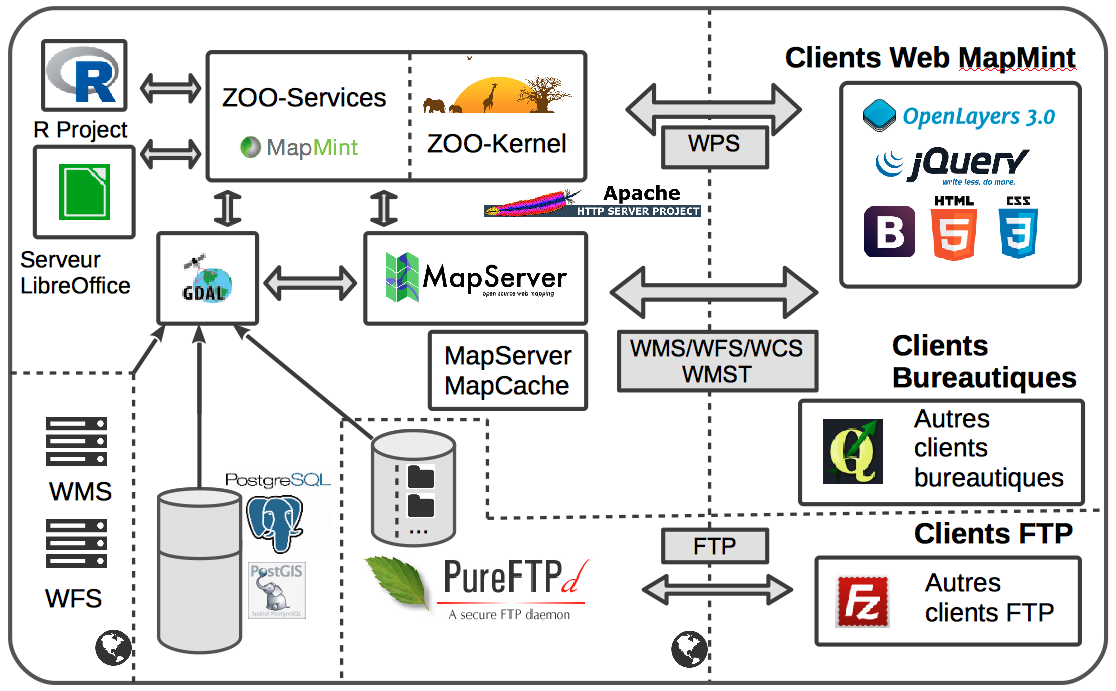
\includegraphics{mapmint-arch.png}

L'interropérabilité de MapMint est assurée par les standards utilisés
et mis en oeuvre. Il est ainsi possible d'interragir avec les données
et services de MapMint, non seulement depuis l'application accessible
depuis un navigateur internet mais aussi depuis un client bureautique
de type QGIS par exemple.

\begin{notice}{note}{Note:}
Pour l'utilisation des services WPS, merci de télécharger le plugin
WPS disponible \href{http://geolabs.fr/plugins.xml}{ici}.
\end{notice}

Retrouvez des informations d'ordre général sur le site internet de \href{http://mapmint.com/en/}{MapMint}


\section{Installer MapMint}
\label{introduction/installmapmint:installer-mapmint}\label{introduction/installmapmint::doc}\label{introduction/installmapmint:introduction-installmapmint}\setbox0\vbox{
\begin{minipage}{0.95\linewidth}
\textbf{Table des matières}

\medskip

\begin{itemize}
\item {} 
\phantomsection\label{introduction/installmapmint:id1}{\hyperref[introduction/installmapmint:installer-mapmint]{\emph{Installer MapMint}}}
\begin{itemize}
\item {} 
\phantomsection\label{introduction/installmapmint:id2}{\hyperref[introduction/installmapmint:prerequis]{\emph{Prérequis}}}
\begin{itemize}
\item {} 
\phantomsection\label{introduction/installmapmint:id3}{\hyperref[introduction/installmapmint:paquets-et-modules-python]{\emph{Paquets et modules Python}}}

\item {} 
\phantomsection\label{introduction/installmapmint:id4}{\hyperref[introduction/installmapmint:telecharger-ansible-et-les-scripts-d-installation]{\emph{Télécharger Ansible et les scripts d'installation}}}

\item {} 
\phantomsection\label{introduction/installmapmint:id5}{\hyperref[introduction/installmapmint:creation-d-une-cle-ssh]{\emph{Création d'une clé SSH}}}

\end{itemize}

\item {} 
\phantomsection\label{introduction/installmapmint:id6}{\hyperref[introduction/installmapmint:installation]{\emph{Installation}}}

\end{itemize}

\end{itemize}
\end{minipage}}
\begin{center}\setlength{\fboxsep}{5pt}\shadowbox{\box0}\end{center}

L'application MapMint peut être installée de manière très simple en
utilisant des scripts \href{http://ansible.com}{Ansible} . Il est donc
possible de déployer plusieures instances de MapMint via l'utilisation
de la commande \code{ansible-playbook}. Dans cette partie l'installation
ne concernera qu'une seule instance, l'hôte local qui utilise une
distribution GNU/Linux : Ubuntu LTS 14.03.3.


\subsection{Prérequis}
\label{introduction/installmapmint:prerequis}

\subsubsection{Paquets et modules Python}
\label{introduction/installmapmint:paquets-et-modules-python}
Avant de pouvoir installer MapMint en utilisant les scripts Ansible, il
est nécessaire de s'assurer de la présence des certains paquets
Ubuntu ainsi que des modules python spécifiques.

\begin{Verbatim}[commandchars=\\\{\}]
sudo apt\PYGZhy{}get install git python\PYGZhy{}setuptools openssh\PYGZhy{}server
sudo easy\PYGZus{}install pip
sudo pip install paramiko PyYAML Jinja2 httplib2 six
\end{Verbatim}


\subsubsection{Télécharger Ansible et les scripts d'installation}
\label{introduction/installmapmint:telecharger-ansible-et-les-scripts-d-installation}
Il est nécessaire de télécharger Ansible et les scripts spécifiques
d'installation de MapMint. Pour ce faire, utilisez les commandes
suivantes.

\begin{Verbatim}[commandchars=\\\{\}]
cd
mkdir mm\PYGZhy{}install
cd mm\PYGZhy{}install
git clone git://github.com/ansible/ansible.git \PYGZhy{}\PYGZhy{}recursive
git clone git://github.com/mapmint/ansible\PYGZhy{}roles mapmint\PYGZhy{}setup
\end{Verbatim}


\subsubsection{Création d'une clé SSH}
\label{introduction/installmapmint:creation-d-une-cle-ssh}
Afin que votre utilisateur puisse se connecter au serveur via SSH sur
lequel installer MapMint, vous devez tout d'abort créer une clé
permettant une authentification automatique. Pour ce faire utiliser
le commande suivante.

\begin{Verbatim}[commandchars=\\\{\}]
mkdir \PYGZti{}/.ssh
ssh\PYGZhy{}keygen \PYGZhy{}t rsa
sudo mkdir /root/.ssh
sudo cp \PYGZti{}/.ssh/id\PYGZus{}rsa.pub /root/.ssh/authorized\PYGZus{}keys
\end{Verbatim}

\begin{notice}{warning}{Avertissement:}
La dernière commande supprime toutes lesclés autorisées du
serveur.
\end{notice}

\begin{notice}{note}{Note:}
Utilisez une commande différente si vous souhaitez mettre à jour la
liste des clés autorisées.
\end{notice}


\subsection{Installation}
\label{introduction/installmapmint:installation}
L'installation de MapMint est entièrement automatisée via les scripts
Ansible téléchargés précédemment, il ne reste donc plus qu'à les
lancer. Avant cela, il sera nécessaire de paramétrer Ansible et les
scripts spécifiques d'installation de MapMint afin de définir le nom
de la machine qui sera utilisé pour accéder à l'instance.

Dans un premier temps vous allez activer Ansible et définir sur
quelles machines vous souhaitez installer MapMint. Dans l'exemple
présenté ici, l'installations sera faite sur la machine local, donc
\code{localhost}.

\begin{Verbatim}[commandchars=\\\{\}]
source \PYGZti{}/mm\PYGZhy{}install/ansible/hacking/env\PYGZhy{}setup
echo \PYGZdq{}localhost\PYGZdq{} \PYGZgt{} \PYGZti{}/ansible\PYGZus{}hosts
sed \PYGZdq{}s:myhost.net:localhost:g\PYGZdq{} \PYGZhy{}i \PYGZbs{}
   \PYGZti{}/mm\PYGZhy{}install/mapmint\PYGZhy{}setup/debian/dependencies/vars/main.yml
export ANSIBLE\PYGZus{}INVENTORY=\PYGZti{}/ansible\PYGZus{}hosts
\end{Verbatim}

\begin{notice}{note}{Note:}
\code{localhost} devrait être remplacer par le nom de machine ou
l'adresse ip permettant l'accès publique à l'instance.
\end{notice}

Il ne reste plus qu'à invoquer l'installation de MapMint avec la
commande ci-dessous.

\begin{Verbatim}[commandchars=\\\{\}]
cd \PYGZti{}/mm\PYGZhy{}install/mapmint\PYGZhy{}setup/ubuntu
ansible\PYGZhy{}playbook \PYGZhy{}s server.yml \PYGZhy{}u root
\end{Verbatim}

Pour accéder à votre instance MapMint, vous pouvez utiliser les liens
suivants :
\begin{itemize}
\item {} 
{\hyperref[introduction/usemapmint:introduction-usemapmint-administration-access]{\emph{Accès aux modules d'administration}}} : \href{http://localhost/ui/Dashboard\_bs}{http://localhost/ui/Dashboard\_bs}

\item {} 
{\hyperref[introduction/usemapmint:introduction-usemapmint-public-access]{\emph{Accès à l'interface publique}}} : \href{http://localhost/ui/public/}{http://localhost/ui/public/}

\end{itemize}


\section{Utiliser MapMint}
\label{introduction/usemapmint:utiliser-mapmint}\label{introduction/usemapmint:introduction-usemapmint}\label{introduction/usemapmint::doc}\setbox0\vbox{
\begin{minipage}{0.95\linewidth}
\textbf{Table des matières}

\medskip

\begin{itemize}
\item {} 
\phantomsection\label{introduction/usemapmint:id1}{\hyperref[introduction/usemapmint:utiliser-mapmint]{\emph{Utiliser MapMint}}}
\begin{itemize}
\item {} 
\phantomsection\label{introduction/usemapmint:id2}{\hyperref[introduction/usemapmint:acces-aux-modules-d-administration]{\emph{Accès aux modules d'administration}}}

\item {} 
\phantomsection\label{introduction/usemapmint:id3}{\hyperref[introduction/usemapmint:formulaire-d-identification]{\emph{Formulaire d'identification}}}

\item {} 
\phantomsection\label{introduction/usemapmint:id4}{\hyperref[introduction/usemapmint:acces-a-l-interface-publique]{\emph{Accès à l'interface publique}}}

\item {} 
\phantomsection\label{introduction/usemapmint:id5}{\hyperref[introduction/usemapmint:premiers-parametrages]{\emph{Premiers paramétrages}}}
\begin{itemize}
\item {} 
\phantomsection\label{introduction/usemapmint:id6}{\hyperref[introduction/usemapmint:titre-de-l-interface-publique]{\emph{Titre de l'interface publique}}}

\item {} 
\phantomsection\label{introduction/usemapmint:id7}{\hyperref[introduction/usemapmint:carte-de-l-interface-publique]{\emph{Carte de l'interface publique}}}

\end{itemize}

\item {} 
\phantomsection\label{introduction/usemapmint:id8}{\hyperref[introduction/usemapmint:ajouter-des-donnees]{\emph{Ajouter des données}}}

\item {} 
\phantomsection\label{introduction/usemapmint:id9}{\hyperref[introduction/usemapmint:acces-aux-donnees-et-traitements-depuis-des-clients-bureautiques]{\emph{Accès aux données et traitements depuis des clients bureautiques}}}
\begin{itemize}
\item {} 
\phantomsection\label{introduction/usemapmint:id10}{\hyperref[introduction/usemapmint:acceder-aux-services-de-diffusion-de-donnees]{\emph{Accéder aux services de diffusion de données}}}

\item {} 
\phantomsection\label{introduction/usemapmint:id11}{\hyperref[introduction/usemapmint:acceder-aux-services-de-traitements-de-donnees]{\emph{Accéder aux services de traitements de données}}}

\end{itemize}

\end{itemize}

\end{itemize}
\end{minipage}}
\begin{center}\setlength{\fboxsep}{5pt}\shadowbox{\box0}\end{center}

L'application MapMint est constituée d'une \textbf{interface
d'administration} comportant différents modules et d'une \textbf{interface
publique}.


\subsection{Accès aux modules d'administration}
\label{introduction/usemapmint:acces-aux-modules-d-administration}\label{introduction/usemapmint:introduction-usemapmint-administration-access}
En fonction des paramètres du {\hyperref[dashboard/configuration::doc]{\emph{\emph{Panneau de configuration}}}} et de
votre installation de MapMint, les modules listés ci-dessous sont
disponibles dans l'interface d'administration.

\begin{tabulary}{\linewidth}{|L|L|}
\hline

\textbf{Module}
 & 
\textbf{URL d'accès}
\\
\hline
Tableau de bord
 & 
\href{http://votre-instance.com/Dashboard\_bs}{http://votre-instance.com/Dashboard\_bs}
\\
\hline
Gestion des données
 & 
\href{http://votre-instance.com/Distiller\_bs}{http://votre-instance.com/Distiller\_bs}
\\
\hline
Création de territoires
 & 
\href{http://votre-instance.com/Territories\_bs}{http://votre-instance.com/Territories\_bs}
\\
\hline
Création d'indicateurs
 & 
\href{http://votre-instance.com/Indexes\_bs}{http://votre-instance.com/Indexes\_bs}
\\
\hline
Création de thèmes
 & 
\href{http://votre-instance.com/Themes\_bs}{http://votre-instance.com/Themes\_bs}
\\
\hline
Importation de documents
 & 
\href{http://votre-instance.com/Documents\_bs}{http://votre-instance.com/Documents\_bs}
\\
\hline
Création de cartes
 & 
\href{http://votre-instance.com/Manager\_bs}{http://votre-instance.com/Manager\_bs}
\\
\hline
Publication d'applications
 & 
\href{http://votre-instance.com/Publisher\_bs}{http://votre-instance.com/Publisher\_bs}
\\
\hline\end{tabulary}



\subsection{Formulaire d'identification}
\label{introduction/usemapmint:formulaire-d-identification}
Pour accèder aux modules de l'interface d'administration, entrez le \textbf{nom d'utilisateur} et le \textbf{mot de passe} qui vous ont été communiqués par email dans le formulaire de connexion illustré ci-après, et cliquez sur le bouton ``Identification''.

\begin{notice}{note}{Note:}
Vous pouvez également presser le bouton ``Entrer'' de votre clavier au lieu de cliquer sur le bouton ``Identifier''
\end{notice}

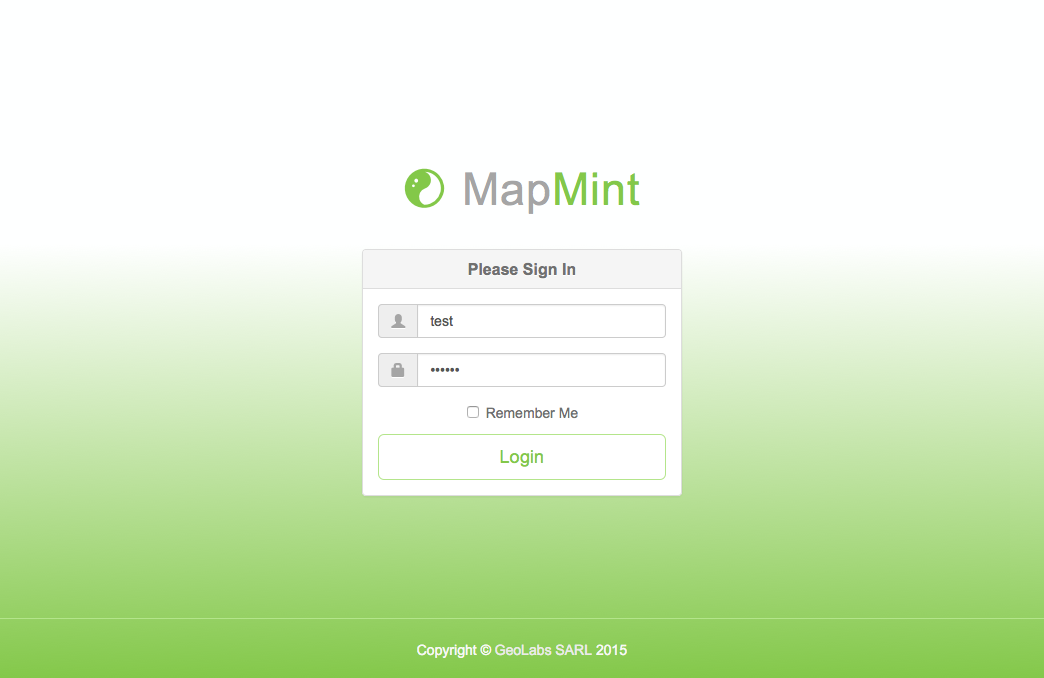
\includegraphics{login-screen.png}

Un message de succès s'affiche dans un cadre vert en haut à droite de votre écran et le module se charge. Si vous obtenez un bandeau rouge en haut de l'écran, veuillez vérifier vos paramètres de connexion et recommencer.


\subsection{Accès à l'interface publique}
\label{introduction/usemapmint:introduction-usemapmint-public-access}\label{introduction/usemapmint:acces-a-l-interface-publique}
L'interface publique de MapMint est accessible via l'URL
\href{http://votre-instance.com/public/}{http://votre-instance.com/public/} qui constitue la page d'accueil de
l'application. Les cartes publiéees sont accessibles depuis la
cartothèque (deuxième onglet du menu). On peut accèder directement à
une carte spécifique en utilisant sont URL spécifique ( du type
\href{http://votre-instance.com/public/le-nom-de-votre-carte}{http://votre-instance.com/public/le-nom-de-votre-carte}).

\begin{tabulary}{\linewidth}{|L|L|}
\hline

\textbf{Module}
 & 
\textbf{URL d'accès}
\\
\hline
Interface publique
 & 
\href{http://votre-instance.com/public/}{http://votre-instance.com/public/}
\\
\hline
Interface publique indicateurs
 & 
\href{http://votre-instance.com/public/indicateurs}{http://votre-instance.com/public/indicateurs}
\\
\hline
Carte publiée
 & 
\href{http://votre-instance.com/public/le-nom-de-votre-carte}{http://votre-instance.com/public/le-nom-de-votre-carte}
\\
\hline\end{tabulary}



\subsection{Premiers paramétrages}
\label{introduction/usemapmint:premiers-parametrages}
Lors d'une première connexion, les étapes suivantes sont recommandées pour  assurer le bon fonctionnement de l'interface publique.


\subsubsection{Titre de l'interface publique}
\label{introduction/usemapmint:titre-de-l-interface-publique}
Le titre de l'interface publique apparait dans le bandeau du haut de la page d'accueil. Pour le configurer, rendez vous dans le {\hyperref[dashboard/configuration::doc]{\emph{\emph{Panneau de configuration}}}} puis modifiez la valeur \textbf{Title} dans l'onglet \emph{Configuration du fournisseur}. Cliquez sur le bouton ``Enregister'' du panneau de configuration et recharger votre page d'accueil pour que les modifications soient effectives.

\begin{notice}{note}{Note:}
Le titre est également utilisé dans la balise \textless{}title\textgreater{} du code source de la page
\end{notice}


\subsubsection{Carte de l'interface publique}
\label{introduction/usemapmint:carte-de-l-interface-publique}
La carte de l'interface publique apparait dans le corps de la page d'accueil. Pour la créer et la configurer, rendez vous dans le {\hyperref[maps/index::doc]{\emph{\emph{Module de création de cartes}}}} puis créer un projet nommé \textbf{Default}. Une fois enregistrée, veuillez recharger cette la page d'accueil pour voir la carte s'afficher.

\begin{notice}{note}{Note:}
La carte d'accueil peut être utilisée pour cartographier un projet en particulier que l'utilisateur souhaiterait voir affichée sur la page d'accueil. Elle peut aussi servir d'entrée cartographique vers les différents projets publiés. Celà nécessite l'utilisation d'une source de données répertoriant les URL des projets.
\end{notice}


\subsection{Ajouter des données}
\label{introduction/usemapmint:ajouter-des-donnees}
Deux solutions sont proposées pour charger des données SIG sur le serveur d'installation de votre instance MapMint.

Si vous souhaitez ajouter des données vectorielles légères (\textbf{\textless{} 2Mo}), rendez vous dans le {\hyperref[data/index::doc]{\emph{\emph{Module de gestion des données}}}} et utiliser l'utilitaire de chargement de données (upload), dont le fonctionnement est décrit dans la section relative aux {\hyperref[data/index::doc]{\emph{\emph{Module de gestion des données}}}}.

Si vous désirez charger des données vecteur ou rester plus volumineuses, il vous faudra utiliser l'accès FTP qui vous a été fournit avec les informations de connexion à votre instance MapMint. Pour ce faire, veuillez installer et lancer un client FTP depuis votre ordinateur (comme \href{https://filezilla-project.org/}{FileZilla} par exemple) et renseigner les informations suivantes dans le formulaire prévu à cet effet (en haut de la fenêtre du logiciel dans le cas de FileZilla), puis cliquer sur le bouton ``Connexion''.

\begin{tabulary}{\linewidth}{|L|L|}
\hline

\textbf{Paramètre}
 & 
\textbf{Définition}
\\
\hline
Hôte
 & 
URL ou adresse IP du serveur sur lequel votre instance est installée
\\
\hline
Nom d'utilisateur
 & 
Nom d'utilisateur fourni par email
\\
\hline
Mot de passe
 & 
Mot de passe fourni par email
\\
\hline\end{tabulary}


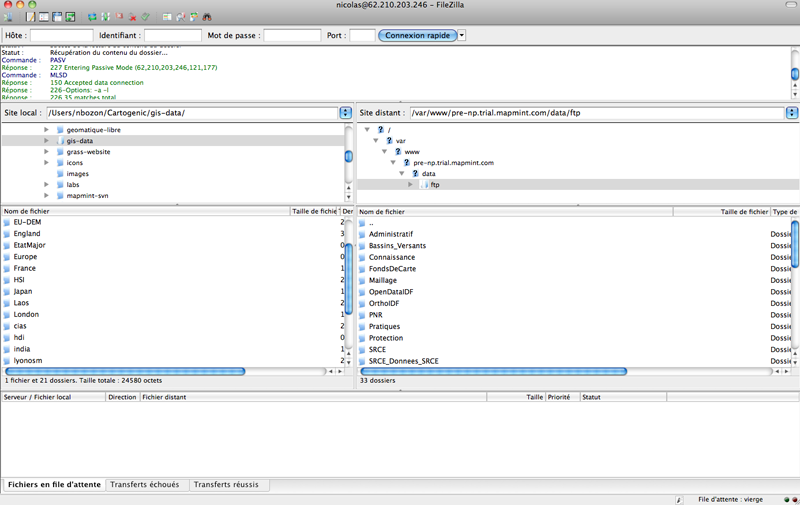
\includegraphics{upload-ftp.png}

Une fois connecté au serveur, le répertoire général de stockage des sources de données (il s'agit générallement du répertoire /var/www/data/ftp) est listé et affiché dans la fenêtre de droite du client FTP. Vous pouvez alors créer un nouveau répertoire ou bien utiliser un répertoire existant.
\begin{itemize}
\item {} 
Dans le cas ou vous souhaiteriez ajouter des données à un répertoire existant, veuillez procéder à un glissé-déposé de vos données de la partie gauche de la fenêtre (où l'arborescence de votre ordinateur est listée) à la partie droite, en direction du répeetoire visé. Cela entraîne le chargement des données dans le répertoire concerné sur le serveur. La progression du chargement des fichiers est indiquée par des barres de progression en bas de la fenêtre. La durée du transfert varie en fonction du poids des données à charger.

\item {} 
Dans le cas ou vous souhaiteriez créer un nouveau répertoire, procédez à un clic droit dans la partie de droite et cliquez sur le sous menu ``Créer un nouveau dossier'' du menu contextuel qui apparait. Entrez ensuite un nom pour le nouveau répertoire dans la fenêtre prévue à cet effet, puis cliquer sur le bouton ``OK''. Cela entraîne la fermeture de la fenêtre et l'ajou du nouveau répertoire à la liste. Vous pouvez ensuite procéder à un glissé-déposé des vos données, comme décrit dans le paragraphe précédent.

\end{itemize}

\begin{notice}{warning}{Avertissement:}
Le nom d'un nouveau répertoire de données ne doit pas contenir d'accents ou de caractères spéciaux !
\end{notice}


\subsection{Accès aux données et traitements depuis des clients bureautiques}
\label{introduction/usemapmint:acces-aux-donnees-et-traitements-depuis-des-clients-bureautiques}
Comme indiqué dans la section {\hyperref[introduction/introduction:userguidegeneral]{\emph{Généralités}}}, MapMint fournis
des services web permettant d'accéder aux données (WMS, WFS et WCS) et
aux services de traitements de données (WPS) depuis des clients
bureautiques, comme par exemple \href{http://www.qgis.org}{QGIS}.

Nous présentons dans cette section comment accéder depuis QGIS aux
services de diffusion de données puis aux services traitements de
données. Nous présenterons aussi successivement comment les utiliser.


\subsubsection{Accéder aux services de diffusion de données}
\label{introduction/usemapmint:acceder-aux-services-de-diffusion-de-donnees}
MapMint rend accessible l'ensemble des espaces de stockages ainsi que
les sources de données qu'elles contiennent une fois ces dernières
paramétrées depuis le {\hyperref[maps/index:maps]{\emph{Module de création de cartes}}}. De même, l'ensemble des
couches contenues dans les applications de cartographie dynamique
configurées depuis le {\hyperref[maps/index:maps]{\emph{Module de création de cartes}}} et publiées depuis le {\hyperref[apps/index:apps]{\emph{Module de publication d'applications}}}
sont elles aussi accéssibles.

Depuis QGIS par exemple, vous pouvez donc accéder aux couches de
données au format WMS, afin de conserver le style que vous avez défini
au niveau du {\hyperref[maps/index:maps]{\emph{Module de création de cartes}}}, ou au fomat WFS, afin d'utiliser les
services de traitements de données vectorielles.

Les URL à utiliser pour paramétrer les accès aux serveur WMS et WFS
sont les suivantes :
\begin{itemize}
\item {} 
pour un espace de stockage \textless{}monRépertoire\textgreater{} :

\code{http://votre-instance.com/cgi-bin/mm/mapserver.cgi?map=/var/data/dirs/\textless{}monRépertoire\textgreater{}/ds\_ows.map}

\item {} 
pour un projet \textless{}monProjet\textgreater{} en cours de paramétrage :

\code{http://votre-instance.com/cgi-bin/mm/mapserver.cgi?map=/var/data/maps/project\_\textless{}monProjet\textgreater{}.map}

\item {} 
pour un projet \textless{}monProjet\textgreater{} publié :

\code{http://votre-instance.com/cgi-bin/mm/mapserver.cgi?map=/var/data/public\_maps/project\_\textless{}monProjet\textgreater{}.map}

\end{itemize}

\begin{notice}{note}{Note:}
il est nécessaire de remplacer \code{\textless{}monProjet\textgreater{}} par le nom d'un projet
et \code{\textless{}monRépertoire\textgreater{}} par le nom d'un espace de stockage
disponible dans {\hyperref[data/index:data]{\emph{Module de gestion des données}}}.
\end{notice}

Les deux captures d'écran ci-dessous présente l'ajout d'un serveur WMS
et WFS.

\begin{tabulary}{\linewidth}{|L|L|}
\hline

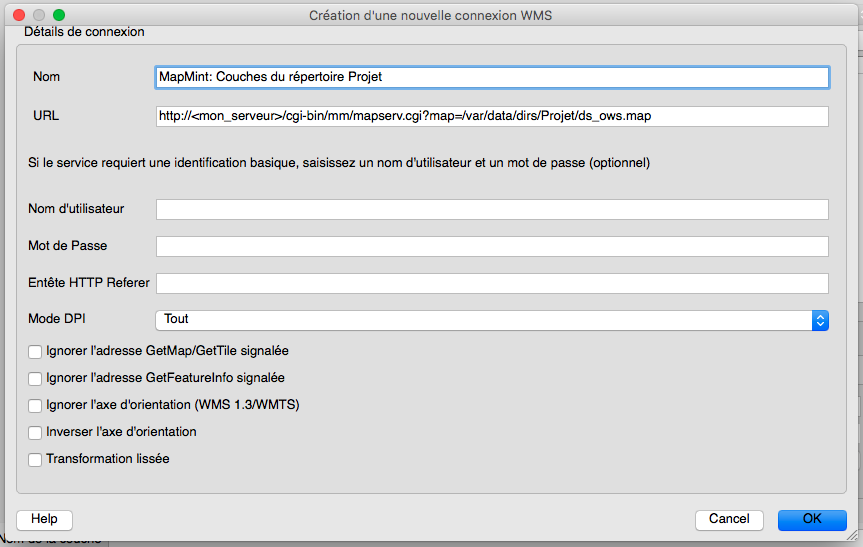
\includegraphics{qgis-wms.png}
 & 
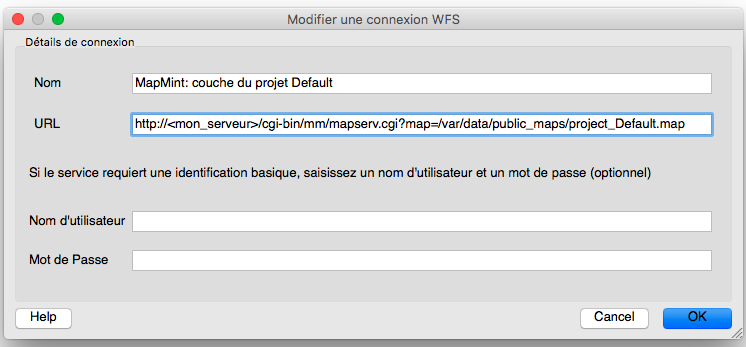
\includegraphics{qgis-wfs.png}
\\
\hline\end{tabulary}


Une fois vos serveurs ajoutés, vous pouvez alors ajouter des couches
qu'ils contiennent. Pour ce faire, sélectionnez vore serveur dans la
liste des serveurs disponibles, puis cliquez sur le bouton
\textbf{Connection} afin de lister les couches disponibles. Ensuite
sélectionné l'ensemble des couches que vous souhaitez afficher dans
votre client QGIS.


\subsubsection{Accéder aux services de traitements de données}
\label{introduction/usemapmint:acceder-aux-services-de-traitements-de-donnees}
Depuis QGIS par exemple, vous pouvez accéder aux services de
traitements de données vectorielles. Pour ce faire il est nécessaire
d'ajouter le serveur suivant \code{http://geolabs.fr/plugins.xml} à vos
dépos de plugins dans QGIS, puis d'installer le module
\textbf{QgsWPSClient}. Une fois ceci fait vous devait alors activer cette
nouvelle extension, puis ajouter un serveur WPS (comme cela a été
présenté dans la section précédente pour les service WMS et
WFS). L'ajout ce fait via l'interface présenté dans la capture d'écran
ci-dessous.

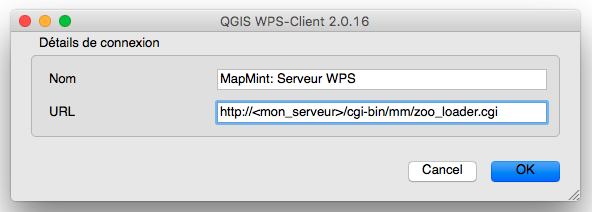
\includegraphics{qgis-wps.png}

L'URL à utiliser pour accéder au services de traitements est le suivant :
\begin{quote}

\code{http://votre-instance.com/cgi-bin/mm/zoo\_loader.cgi}
\end{quote}

Une fois le serveur WPS ajouté, sélectionnez le dans la liste puis
cliquez sur le bouton \textbf{Connect} afin de lister l'esemble des
services de traitements disponibles comme présenté ci-dessous.

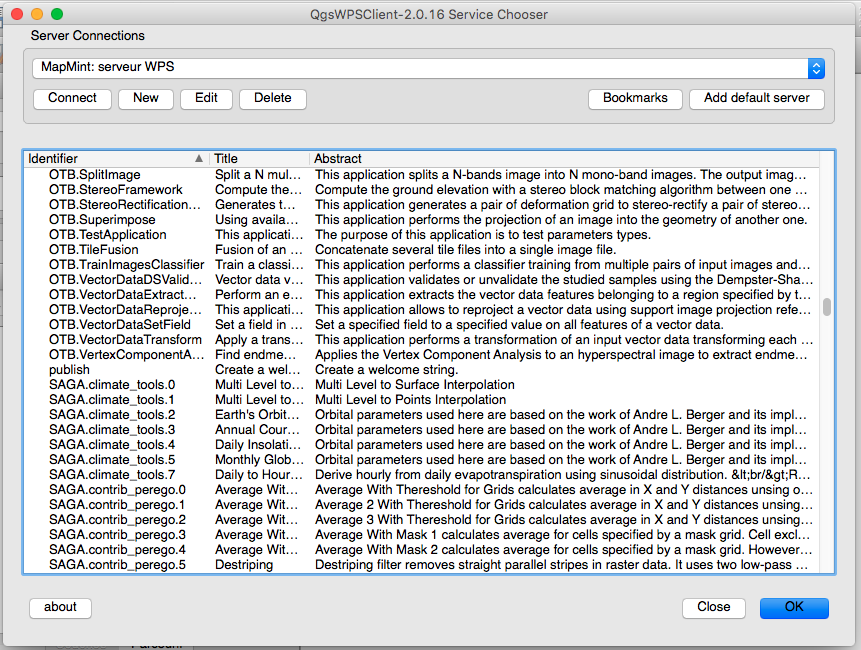
\includegraphics{qgis-wps-gc.png}

Vous devez selectionner un services a exécuter en cliquant deux fois
sur le service qui vous interresse afin d'accéder à l'interface de
passage de paramètres au service WPS. Cette interface correspond à la
capture d'écran suivante.

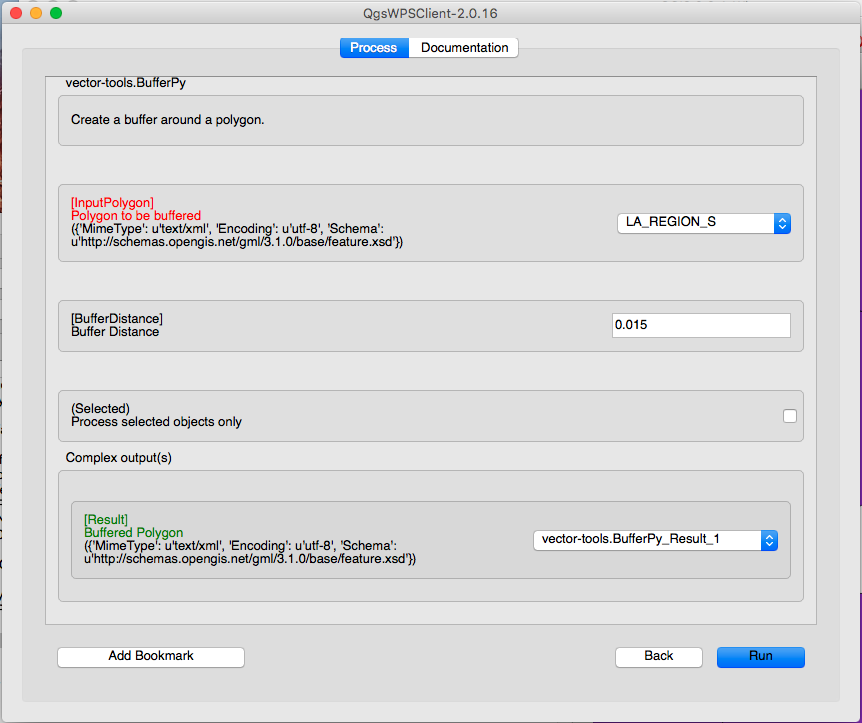
\includegraphics{qgis-wps-buff.png}

\begin{notice}{warning}{Avertissement:}
Seules les couches WFS et WCS peuvent être utilisées avec les
services traitements WPS.
\end{notice}

Afin d'exécuter et d'afficher le résultat, vous devez cliquer sur le
boutton \textbf{Run}.

Nous présentons ci-desous un exemple d'utilisation d'une couche
vectorielle \textbf{LA\_REGION\_S} et de l'exécution des services
\textbf{vector-tools.BufferPy} et \textbf{vector-tools.CentroidPy}.

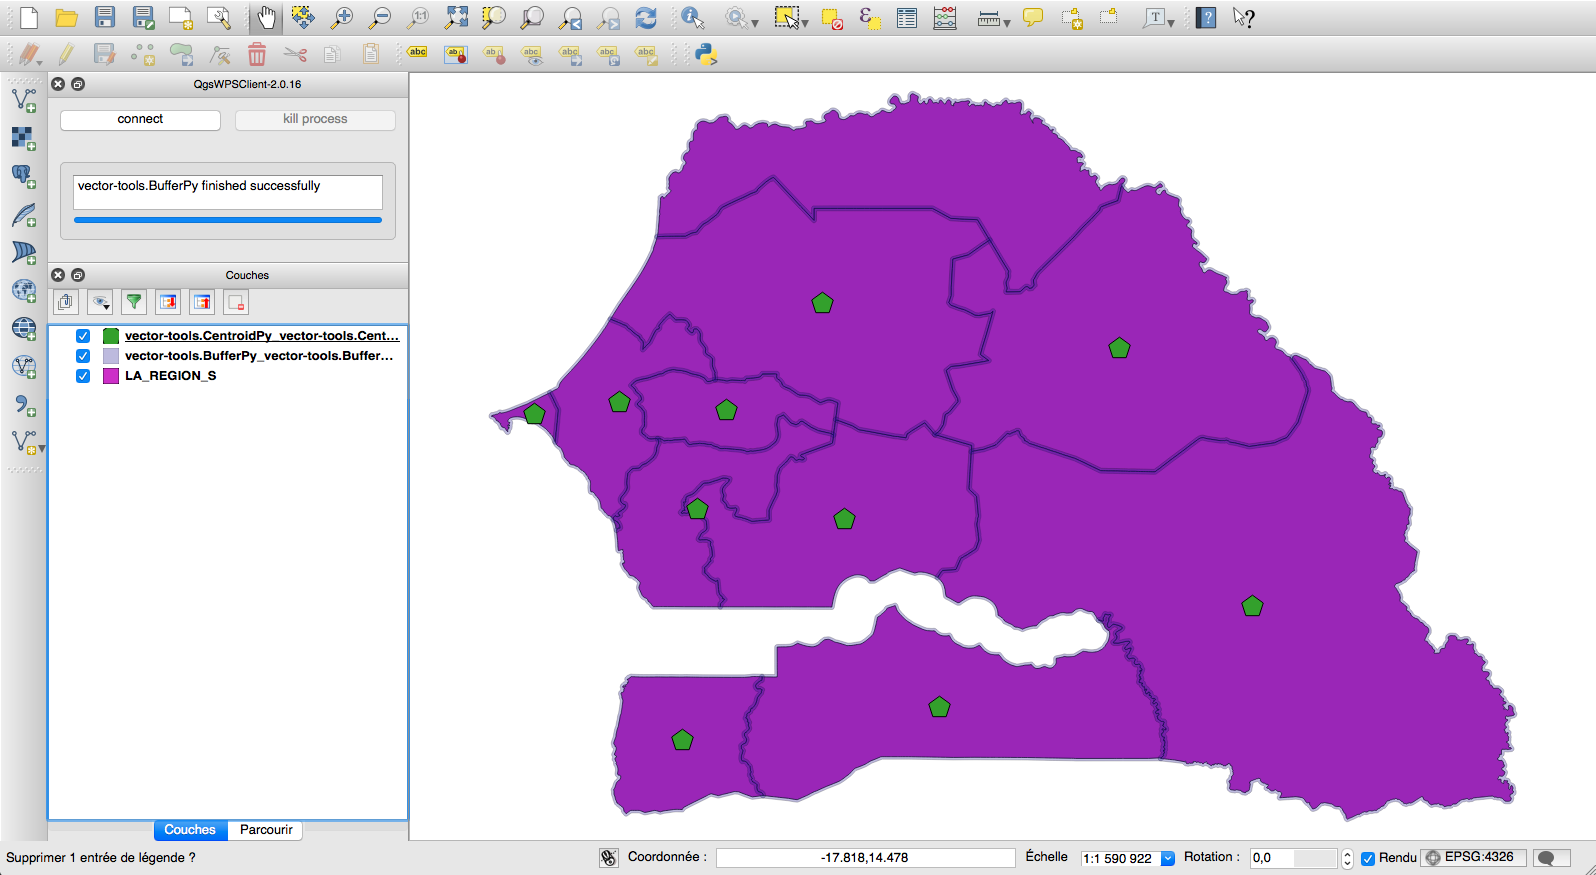
\includegraphics{qgis-wps-result.png}
..


\chapter{Tableau de bord}
\label{dashboard/index:tableau-de-bord}\label{dashboard/index::doc}\label{dashboard/index:dashboard}
Cette section regroupe la documentation relative au tableau de bord de
MapMint.

Le tableau de bord de MapMint est constitué de 3 sections spécifiques
:
\begin{itemize}
\item {} 
\textbf{Vue d'ensemble} : qui est le contenu visible au chargement de la page,

\item {} 
\textbf{Utilisateurs} qui permet la gestion des utilisateurs et des groupes d'utilisateurs,

\item {} 
\textbf{Paramétrage}  qui permet la gestion des paramètres de l'application.

\end{itemize}

\begin{notice}{warning}{Avertissement:}
Il est important de noter ici que seul les utilisateurs des groupes
\textbf{super admin} sont autorisés à accéder aux modules
{\hyperref[dashboard/usersmanagement:dashboard-usersmanagement]{\emph{Gestion des utilisateurs}}} et  {\hyperref[dashboard/configuration:dashboard-configuration]{\emph{Panneau de configuration}}}
\end{notice}


\section{Section ``Vue d'ensemble''}
\label{dashboard/overview::doc}\label{dashboard/overview:section-vue-d-ensemble}\label{dashboard/overview:dashboard-overview}
Le panneau ``Vue d'ensemble'' du {\hyperref[dashboard/index::doc]{\emph{\emph{Tableau de bord}}}} fournit une
vision d'ensemble de l'instance MapMint à un des administrateurs de
l'application.

La date et l'heure de votre dernière connexion à l'instance sont
premièrement indiquées en haut à gauche.

Différents panneaux présentent des informations spécifiques relatives
à l'instance de MapMint, ils sont décrits dans les sections suivantes.

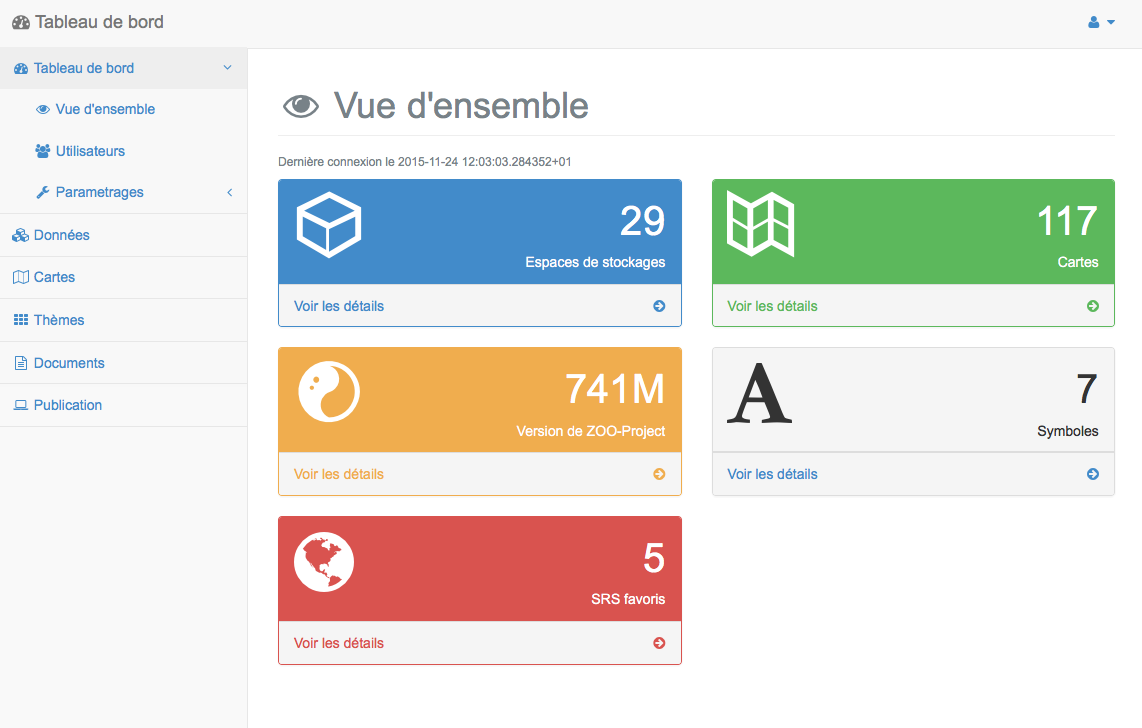
\includegraphics[width=1.000\linewidth]{dashboard-module-preview.png}


\subsection{Données disponibles}
\label{dashboard/overview:donnees-disponibles}
Des informations relatives au {\hyperref[data/index::doc]{\emph{\emph{Module de gestion des données}}}} sont disponibles
dans la panneau bleu présenté ci-dessous, il informe l'administrateur sur:
\begin{itemize}
\item {} 
Le nombre d'espaces de stockages créés

\item {} 
Le nombre de répertoires et de bases de données

\item {} 
Le nombre de sources de données disponibles

\end{itemize}

Une boutton vous permet d'accéder directement au {\hyperref[data/index::doc]{\emph{\emph{Module de gestion des données}}}}.

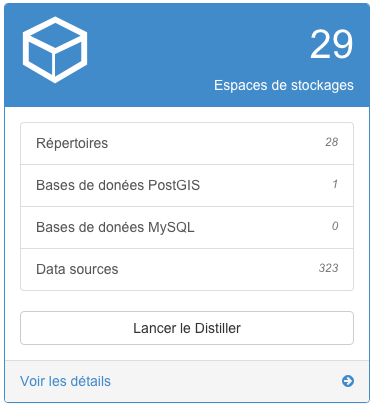
\includegraphics[width=0.330\linewidth]{dashboard-datastore-block.png}


\subsection{Nombres de cartes disponibles}
\label{dashboard/overview:nombres-de-cartes-disponibles}
Le panneau vert présenté ci-dessous, permet d'obtenir un rapide
apperçu des cartes en cours d'édition. En cliquant sur la stylo de la
ligne d'une carte, vous pouvez charger cette carte dans le {\hyperref[maps/index::doc]{\emph{\emph{Module de création de cartes}}}}

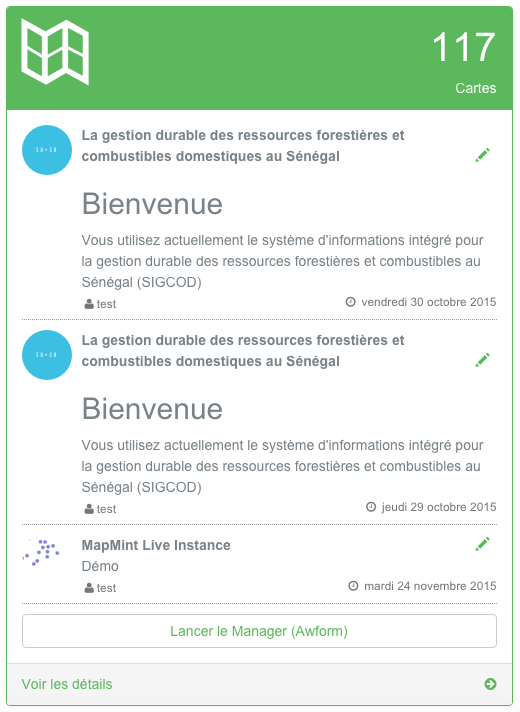
\includegraphics[width=0.330\linewidth]{dashboard-manager-block.png}


\subsection{Versions des logiciels installés}
\label{dashboard/overview:versions-des-logiciels-installes}
Le panneau orange présenté ci-dessous, fournit les informations
relatives aux versions des logiciels installés et utilisés par
l'application MapMint.

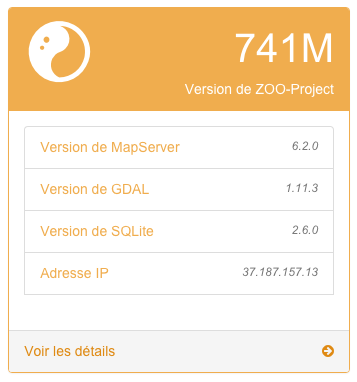
\includegraphics[width=0.330\linewidth]{dashboard-version-block.png}

Cela permet lors de rapport de problème de spécifier les versions utilisées.


\subsection{Gestion des symboles}
\label{dashboard/overview:gestion-des-symboles}
Le panneau gris présenté ci-dessous liste :
\begin{itemize}
\item {} 
les symboles que vous pourrez utiliser pour définir le style de vos couches depuis le {\hyperref[data/index::doc]{\emph{\emph{Module de gestion des données}}}},

\item {} 
les polices disponibles dans une liste déroulante,

\item {} 
la liste des symboles d'une police sélectionnée.

\end{itemize}

Il permet la gestion des symboles utilisés pour définir le style de
vos couches. Le mode opératoire de ce panneau est très simple.
Si vous selectionnez une police présente dans la liste déroulante au
milieu du panneau, l'ensemble des symboles qu'elle contient sera alors
affiché en desous. Vous avez la possibilité de sélectionner un ou plusieur
symboles dans la liste des symboles présents dans une police et de les
ajouter à la liste des symboles disponibles en cliquant sur le boutton
``+''. De la même manière, vous avez la possibilité de sélectionner des
symboles affichés au dessus de la liste déroulante et de cliquer sur
le bouton ``-'' afin de les supprimer effectivement.

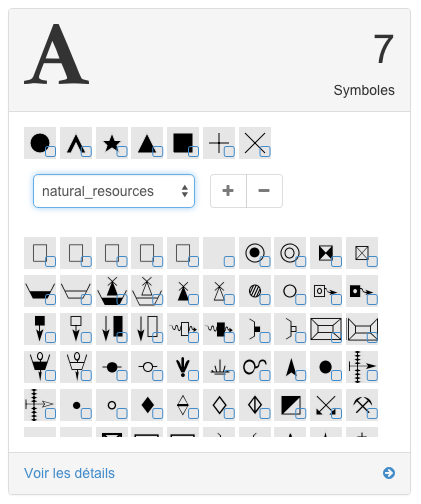
\includegraphics[width=0.330\linewidth]{dashboard-symbols-block.png}


\subsection{Gestion des Systèmes de Références Spatiales (SRS)}
\label{dashboard/overview:gestion-des-systemes-de-references-spatiales-srs}
Le panneau rouge vous présente la liste des Systèmes de Références
Spatiales (SRS). Si vous saisissez un code EPSG ou IGNF dans le champ
affiché en bas du panneau, vous pourrez alors l'ajouter à la liste des
SRS favoris. En cliquant sur le bouton ``poubelle'' vous pouvez
supprimer le SRS correspondant de la liste des favoris. Cela est
utilsé afin de limiter le nombre de SRS affichés dans les divers
formulaires de l'application.

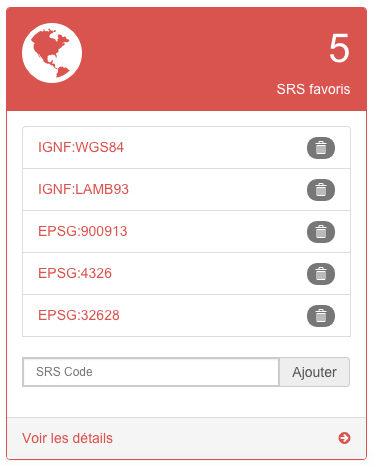
\includegraphics[width=0.330\linewidth]{dashboard-srs-block.png}


\section{Gestion des utilisateurs}
\label{dashboard/usersmanagement:gestion-des-utilisateurs}\label{dashboard/usersmanagement::doc}\label{dashboard/usersmanagement:dashboard-usersmanagement}
La section de gestion des utilisteurs permet de créer, d'éditer et de
supprimer des utilisateurs et des groupes d'utilisateurs.

La page est organisée en deux onglets, ``Utilisateurs'' et ``Groupes''. Un
clic sur le titre de l'onglet entraine l'affichage de la table correspondante.

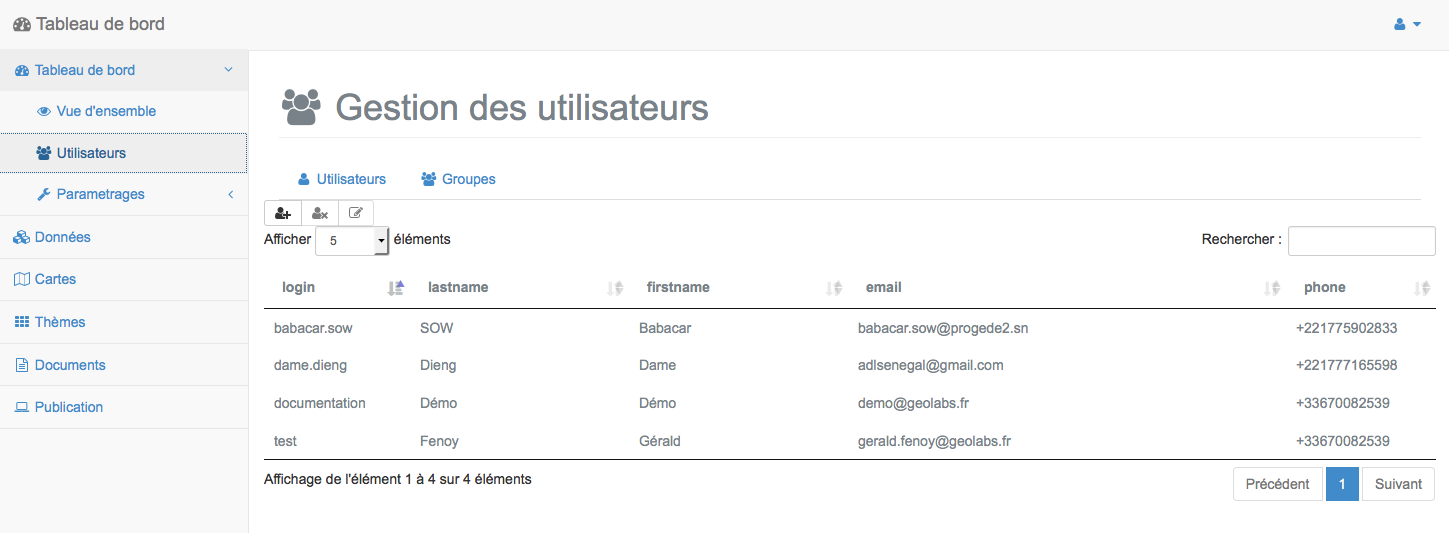
\includegraphics[width=1.000\linewidth]{manage-users-preview.png}

Chaque onglet dispose de la même barre d'outils comportant trois boutons décrits ci-après.

\begin{tabulary}{\linewidth}{|L|L|}
\hline

\textbf{Icône}
 & 
\textbf{Action}
\\
\hline

\includegraphics{add-user.png}
 & 
Affiche le formulaire d'ajout d'un utilisateur/groupe
\\
\hline

\includegraphics{pencil.png}
 & 
Affiche le formulaire d'édition d'un utilisateur/groupe
\\
\hline

\includegraphics{delete-user.png}
 & 
Affiche le formulaire de suppression d'un utilisateur/groupe
\\
\hline\end{tabulary}



\subsection{Ajouter un utilisateur}
\label{dashboard/usersmanagement:ajouter-un-utilisateur}
Pour ajouter un nouvel utilisateur, veuillez cliquer sur le bouton
``Ajouter'' à gauche de la barre d'outils. Celà entraine l'affichage du
formulaire d'ajout d'un utilisateur. Veuillez renseigner tout les champs
puis cliquer sur le bouton ``Ajouter''.

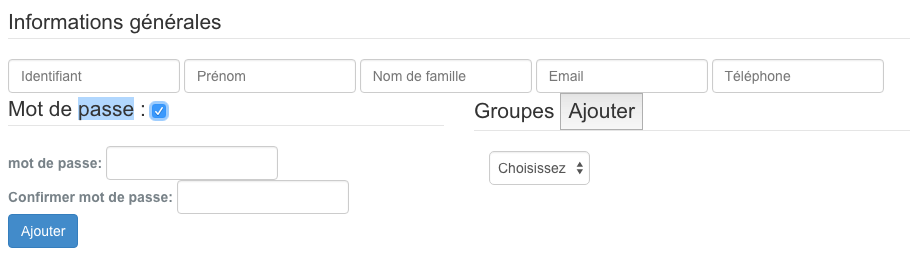
\includegraphics[width=1.000\linewidth]{dashboard-adduser-form.png}

\begin{tabulary}{\linewidth}{|L|L|}
\hline

\textbf{paramètre}
 & 
\textbf{définition}
\\
\hline
Identification
 & 
Définit le nom d'utilisateur pour l'identification
\\
\hline
Nom
 & 
Définit le nom pour du profil utilisateur
\\
\hline
Prénom
 & 
Définit le prénom du profil utilisateur
\\
\hline
Mot de passe
 & 
Définit le mot de passe pour l'identification
\\
\hline
Courriel
 & 
Définit l'adresse éléctronique du profil utilisateur
\\
\hline
Téléphone
 & 
Définit le numéro de téléphone du profil utilisateur
\\
\hline
Groupe
 & 
Définit le/les groupe(s) de l'utilisateur
\\
\hline\end{tabulary}


\begin{notice}{warning}{Avertissement:}
Tous les champs doivent être renseignés pour créer le compte utilisateur.
\end{notice}

\begin{notice}{warning}{Avertissement:}
Vérifiez les droits nécessaires à l'utilisateur et assignez lui un groupe.
\end{notice}

\begin{notice}{note}{Note:}
Le groupe ``public'' correspond aux utilisateurs non connectés de l'interface public.
\end{notice}

\begin{notice}{note}{Note:}
Le champ téléphone supporte les valeurs de type +33100000000
\end{notice}


\subsection{Editer un utilisateur}
\label{dashboard/usersmanagement:editer-un-utilisateur}
Pour éditer un utilisateur, veuillez cliquer sur une ligne du tableau
des utilisateurs. Cette dernière est alors mise en évidence (couleur
verte). Cliquez ensuite sur le bouton ``Editer'' de la barre d'outils,
ce qui entraine l'affichage du formulaire d'édition de l'utilisateur
correspondant.

Tous les paramètres de l'utilisateur sont modifiables. Cliquez sur le
bouton ``Sauver'' pour sauvegarder les modifications, qui seront
signalées dans un bandeau vert en haut de l'écran.

\scalebox{0.800000}{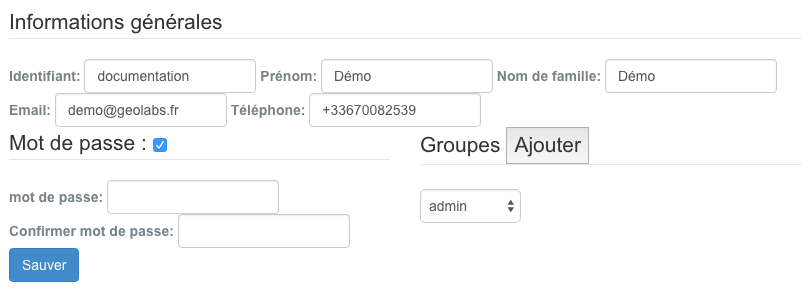
\includegraphics{edit-user-window.png}}

\begin{notice}{warning}{Avertissement:}
La modification du groupe de l'utilisateur modifie ses droits
\end{notice}


\subsection{Supprimer un utilisateur}
\label{dashboard/usersmanagement:supprimer-un-utilisateur}
Pour supprimer un utilisateur, cliquez sur la ligne du tableau
correspondante puis cliquez sur le bouton ``Supprimer''. Cela entraine
l'affichage du formulaire de suppression d'un utilisateur, illustré
ci-dessous.

\scalebox{0.800000}{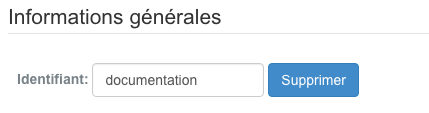
\includegraphics{delete-user-window.png}}

Cliquez ensuite sur le bouton ``Supprimer'' pour supprimer l'utilisateur de la base de données.

\begin{notice}{warning}{Avertissement:}
La suppression d'un utilisateur est définitive !
\end{notice}


\subsection{Ajouter un groupe}
\label{dashboard/usersmanagement:ajouter-un-groupe}
Pour créer un nouveau groupe d'utilisateur, veuillez cliquer sur
l'onglet ``Groupes'' en haut de la fenêtre de gestion des utilisateurs,
puis cliquer sur le bouton ``Ajouter'' de la barre d'outils. Celà
entraine l'affichage du formulaire d'ajout d'un groupe, illustré
ci-dessous.

\scalebox{0.800000}{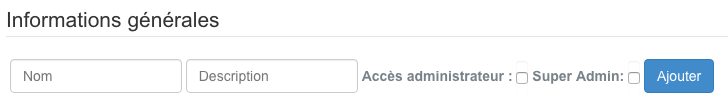
\includegraphics{add-usergroup-window.png}}

\begin{tabulary}{\linewidth}{|L|L|}
\hline

\textbf{Paramètre}
 & 
\textbf{Définition}
\\
\hline
Nom
 & 
Définit le nom du groupe
\\
\hline
Description
 & 
Définit le groupe par une courte phrase
\\
\hline
Accès admin
 & 
Définit si le groupe dispose d'un accès administrateur
\\
\hline
Super Admin
 & 
Définit si le groupe dispose d'un accès super administrateur
\\
\hline\end{tabulary}


Veuillez renseigner tous les champs listés dans le tableau ci-dessus,
puis cliquer sur le bouton ``Ajouter''. Celà entraine la disparission du formulaire, l'ajout du groupe dans le tableau puis le rechargement de la page. Ouvrez à nouveau la fenêtre de gestion des utilisateurs et l'onglet ``Groupe'' pour constater l'ajout du nouveau groupe.

\begin{notice}{note}{Note:}
L'ajout d'utilisateurs lors de la création du groupe est facultative
\end{notice}

\begin{notice}{note}{Note:}
Les groupes ayant le paramètre \textbf{Super Admin} coché sont les super
administrateurs, ils ont donc un accès complet au paramétrage et à
la gestion des utilisateurs.
\end{notice}


\subsection{Editer un groupe}
\label{dashboard/usersmanagement:editer-un-groupe}
Pour éditer un groupe, veuillez cliquer sur une ligne du tableau
correspondant. Cette dernière est alors mise en évidence (couleur
bleue). Cliquez ensuite sur le bouton “Editer” de la barre d’outils,
ce qui entraine l’affichage du formulaire d’édition du groupe
d'utilisateurs correspondant.

Tous les paramètres du groupe sont modifiables. Cliquez sur le bouton
“Sauver” pour enregistrer les modifications.

\scalebox{0.800000}{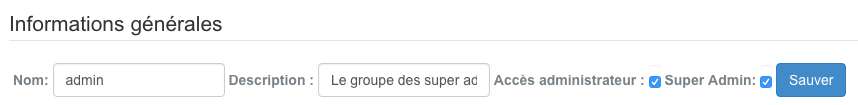
\includegraphics{edit-usergroup-window.png}}


\subsection{Supprimer un groupe}
\label{dashboard/usersmanagement:supprimer-un-groupe}
Pour supprimer un groupe d'utilisateurs, cliquez sur la ligne du
tableau correspondant puis cliquez sur le bouton “Supprimer”. Cela
entraine l’affichage du formulaire de suppression d’un groupe
utilisateur, comme illustré ci-dessous.

\scalebox{0.800000}{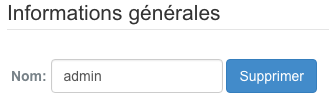
\includegraphics{delete-usergroup-window.png}}

Le nom du groupe est spécifié dans un champ texte, cliquez sur le bouton ``Supprimer'' pour supprimer le groupe. Celà entraine la fermeture de la fenêtre, la suppression du groupe dans le tableau puis le rechargement de la page.

\begin{notice}{warning}{Avertissement:}
La suppression d'un groupe d'utilisateurs est définitive !
\end{notice}


\section{Panneau de configuration}
\label{dashboard/configuration::doc}\label{dashboard/configuration:panneau-de-configuration}\label{dashboard/configuration:dashboard-configuration}
Le panneau de configuration permet de visualiser et d'éditer les
paramètres d'installation de MapMint. Les formulaires sont renseignés
automatiquement par rapport au contenu du fichier de paramétrage
\code{main.cfg}.

\begin{notice}{warning}{Avertissement:}
Il n'est pas conseillé de modifier les paramètres de configuration sans en connaitre les conséquences
\end{notice}

Le panneau de configuration est organisé en 4 sections, listés ci-dessous. Un clic sur l'icône entraine l'affichage de l'onglet correspondant.

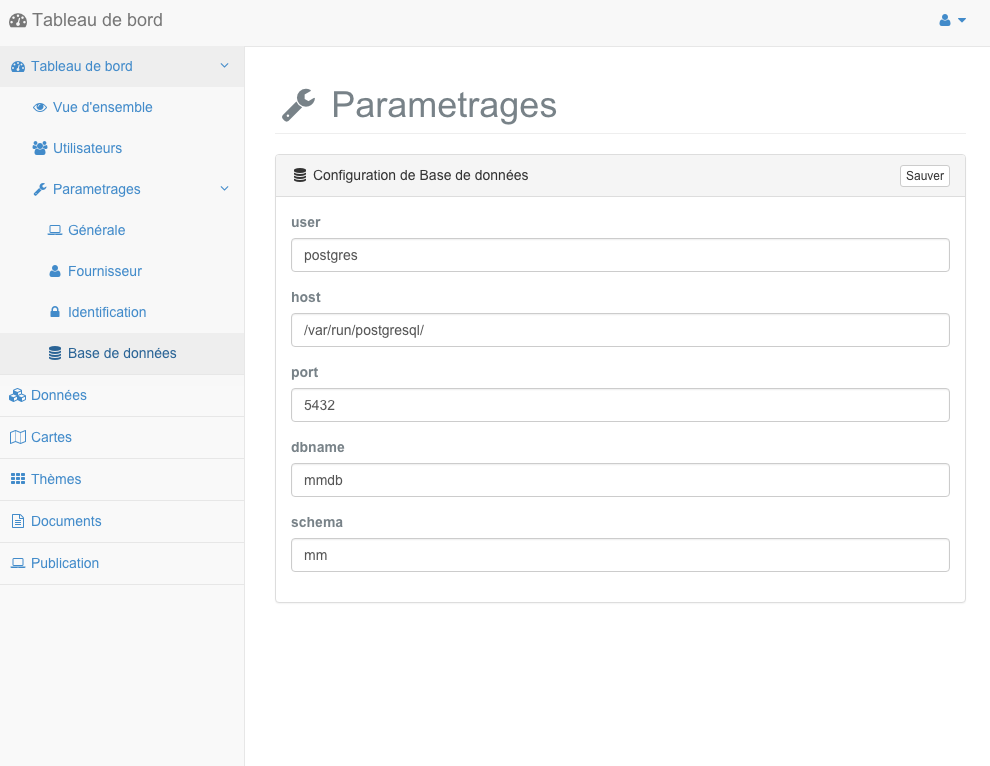
\includegraphics[width=1.000\linewidth]{dashboard-conf-form.png}

Comme présenté dans la capture d'écran précédente, une fois que vous
avez édité les paramètres de configuration, vous pouver utiliser le
bouton ``Sauver'' en haut à droite du panneau pour enregistrer vos
modifications.

\begin{tabulary}{\linewidth}{|L|L|}
\hline

\textbf{Icône}
 & 
\textbf{Action}
\\
\hline

\includegraphics{monitor.png}
 & 
Configuration générale
\\
\hline

\includegraphics{security.png}
 & 
Configuration de l'identification
\\
\hline

\includegraphics{user.png}
 & 
Configuration du fournisseur
\\
\hline

\includegraphics{db.png}
 & 
Configuration de la base de données
\\
\hline\end{tabulary}



\subsection{Configuration générale}
\label{dashboard/configuration:configuration-generale}
Le formulaire de confuguration générale regroupe les variables d'environnement et les paramètres d'installation de l'instance MapMint.

\begin{tabulary}{\linewidth}{|L|L|}
\hline

\textbf{Paramètre}
 & 
\textbf{Définition}
\\
\hline
Encoding
 & 
Définit l'encodage de l'installation par défaut (utf-8)
\\
\hline
Mmadress
 & 
Définit l'URL d'accès à l'instance par défaut (/mm/)
\\
\hline
Datapath
 & 
Définit le chemin vers le répertoire /data dédié aux stockage des données
\\
\hline
Jscache
 & 
Définit si les fichiers javascripts sont compressés ou non (prod\textbar{}dev)
\\
\hline
Tmppath
 & 
Définit le chemin vers le répertoire de stockage des fichiers temporaires (/tmp/)
\\
\hline
Cachedir
 & 
Définit le chemin vers le répertoire de stockage du cache (/cache/)
\\
\hline
3D
 & 
Définit l'activation du mode 3D (false\textbar{}true)
\\
\hline
Rooturl
 & 
Définit l'URL d'accès à l'interface publique par défaut (/public/)
\\
\hline
Publicationurl
 & 
Définit l'URL de publication où sont stockés les fichiers (/public\_map/)
\\
\hline
Dblink
 & 
Définit le chemin vers la base de données des utilisateurs de l'instance MapMint
\\
\hline
Mmpath
 & 
Définit l'URL complète du répertoire d'installation par défaut (/mm/)
\\
\hline
Version
 & 
Définit le numéro de version de MapMint
\\
\hline
Rpy2
 & 
Définit l'activation de la librairie R (true\textbar{}false)
\\
\hline
Dbuser
 & 
Définit le nom de la section correspondante aux paramétres de la base de données
\\
\hline
Applicationadress
 & 
Définit l'adresse racine de l'instance MapMint
\\
\hline
Lang
 & 
Définit les langues supportées par l'instance
\\
\hline
Sesspath
 & 
Définit le chemin vers le répertoire de stockage des fichiers temporaires de session (/tmp/)
\\
\hline
Publicationpath
 & 
Définit le chemin vers le répertoire de publication de l'instance MapMint
\\
\hline
Csscache
 & 
Définit si les fichiers CSS sont compressés ou non (prod\textbar{}dev)
\\
\hline
Msogcversion
 & 
Définit la version des services WMS et WFS de MapServer
\\
\hline
Serveradress
 & 
Définit l'URL permettant d'accéder à l'executable de ZOO-Project (WPS kernel)
\\
\hline
Dbusername
 & 
Définit le nom de l'espace de stockage correspondant à la base de données des utilisateurs
\\
\hline
Templatesadress
 & 
Définit l'URL permettant d'accéder au fichiers models générés par l'application (pour les fenêtres et les info bulles)
\\
\hline
Language
 & 
Définit la langue de l'instance
\\
\hline
Mapserveradress
 & 
Définit l'URL permettant d'accéder à l'éxécutable de MapServer
\\
\hline
Tmpurl
 & 
Définit l'URL d'acccès au répertoire temporaire (correspondant au chemin tmpPath)
\\
\hline
Templatespath
 & 
Définit le chemin complet vers le répertoire mapmint-ui/templates
\\
\hline\end{tabulary}



\subsection{Configuration de l'identification}
\label{dashboard/configuration:configuration-de-l-identification}
Les formulaires de configuration de l'identification et du fournisseur des services permettent de caractériser l'organisation qui publie les données et la personne responsable du serveur et/ou de l'application MapMint.

\begin{tabulary}{\linewidth}{|L|L|}
\hline

\textbf{Paramètre}
 & 
\textbf{Définition}
\\
\hline
Positionname
 & 
Définit la position du contact de référence
\\
\hline
Individualname
 & 
Définit le nom individuel du contact de référence
\\
\hline
Providername
 & 
Définit le nom du fournisseur des services
\\
\hline
Adressadministrativearea
 & 
Définit le secteur administratif du fournisseur des services
\\
\hline
Adresscountry
 & 
Définit le pays du fournisseur des services
\\
\hline
Phonevoice
 & 
Définit le numéro de téléphone du contact de référence
\\
\hline
Adresspostalcode
 & 
Définit le code postal du fournisseur des services
\\
\hline
Role
 & 
Définit le role du fournisseur des services
\\
\hline
Providersite
 & 
Définit l'adresse du site Internet du fournisseur des services
\\
\hline
Phonefacsimile
 & 
Définit le numéro de fax du contat de référence
\\
\hline
Addresselectronicmailaddress
 & 
Définit l'adresse de courier électronique du contat de référence
\\
\hline
Adresscity
 & 
Définit la ville du fournisseur des services
\\
\hline
Adressdeliverypoint
 & 
Définit l'adresse du fournisseur des services
\\
\hline\end{tabulary}


\begin{notice}{note}{Note:}
Ces paramètres sont utilisés pour définir les métadonnées ``opengeospatial web services'' (OWS) définies par l'Open Geospatial Consortium  (OGC).
\end{notice}

\begin{notice}{note}{Note:}
Le contact de référence correspond habituellement au nom de la personne responsable du serveur
\end{notice}


\subsection{Configuration du fournisseur des services}
\label{dashboard/configuration:configuration-du-fournisseur-des-services}
\begin{tabulary}{\linewidth}{|L|L|}
\hline

\textbf{Paramètre}
 & 
\textbf{Définition}
\\
\hline
Keywords
 & 
Définit les mots clés attribués aux services web, séparés par des virgules
\\
\hline
Title
 & 
Définit le titre du serveur cartographique
\\
\hline
Abstract
 & 
Définit le serveur cartographique par une courte description
\\
\hline
Accesscontraints
 & 
Définit si le serveur cartographique nécessite une identification
\\
\hline
Fees
 & 
Définit les conditions d'utilisation et/ou le copyright du serveur
\\
\hline\end{tabulary}


\begin{notice}{note}{Note:}
Ces paramètres sont utilisés pour définir les métadonnées ``opengeospatial web services'' (OWS) définies par l'Open Geospatial Consortium  (OGC).
\end{notice}

\begin{notice}{note}{Note:}
Le fournisseur des services correspond habituellement au nom de l'organisme qui publie les données
\end{notice}

\begin{notice}{warning}{Avertissement:}
Le titre et la description du serveur sont également utilisés dans la page d'accueil de l'interface publique
\end{notice}


\subsection{Configuration de la base de données}
\label{dashboard/configuration:configuration-de-la-base-de-donnees}
La page de configuration de la base de données n'est disponible que
lorsque vous utilisez une base de type PostgreSQL pour stocker les
informations des utilisateurs. Dans le cas où vous n'utiliseriez que
la base de données SQLite, cette section ne devrait pas apparaitre.

\begin{tabulary}{\linewidth}{|L|L|}
\hline

\textbf{Paramètre}
 & 
\textbf{Définition}
\\
\hline
user
 & 
Définit le nom d'utilisateur à utiliser pour se connecter au serveur de bases de données
\\
\hline
host
 & 
Définit le nom de machine ou le scoket de domaine unix à utiliser pour se connecter au serveur de bases de données
\\
\hline
port
 & 
Définit le port à utiliser pour se connecter au serveur de bases de données
\\
\hline
dbname
 & 
Définit le nom de la base de données à utiliser
\\
\hline
schema
 & 
Définit le schema de stockage utilisé pour les tables du système
\\
\hline
password
 & 
Définit le mot de passe à utiliser pour se connecter au serveur de bases de données
\\
\hline\end{tabulary}



\chapter{Module de gestion des territoires}
\label{territories/index:territories}\label{territories/index::doc}\label{territories/index:module-de-gestion-des-territoires}
Cette section regroupe la documentation relative au module de gestion des territoires de MapMint.

Le module de gestion des territoires permet de gérer une hierarchie de
territoires qui sera par la suite utilisée dans le module de gestion
des indicateurs permettant de joindre un territoire à une source de
données tierce (base de données, requéte ou autres fichiers XLS,CSV ...).

La page du module est divisée en deux parties :
\begin{itemize}
\item {} 
la partie de gauche appelée le {\hyperref[territories/territorieslist::doc]{\emph{\emph{Panneau des territoires}}}}, il liste l'ensemble des territoires créés et permet l'ajout et la suppression de territoires

\item {} 
la partie de droite appelée le {\hyperref[territories/infopanel::doc]{\emph{\emph{Panneau d'information}}}}, il permet de saisir les informations relatives à un document

\end{itemize}


\section{Panneau des territoires}
\label{territories/territorieslist:territories-territorieslist}\label{territories/territorieslist:panneau-des-territoires}\label{territories/territorieslist::doc}
Un territoire est constitué d'un nom et d'une source de données géographique présente dans la base de données PostGIS de votre instance MapMint. Les territoires sont utilisés comme paramétres d'entrée du {\hyperref[indicators/index::doc]{\emph{\emph{Module de création d'indicateurs}}}}.
\setbox0\vbox{
\begin{minipage}{0.95\linewidth}
\textbf{Table des matiéres}

\medskip

\begin{itemize}
\item {} 
\phantomsection\label{territories/territorieslist:id1}{\hyperref[territories/territorieslist:panneau-des-territoires]{\emph{Panneau des territoires}}}
\begin{itemize}
\item {} 
\phantomsection\label{territories/territorieslist:id2}{\hyperref[territories/territorieslist:ajouter-un-nouveau-territoire]{\emph{Ajouter un nouveau territoire}}}

\item {} 
\phantomsection\label{territories/territorieslist:id3}{\hyperref[territories/territorieslist:supprimer-un-territoire]{\emph{Supprimer un territoire}}}

\end{itemize}

\end{itemize}
\end{minipage}}
\begin{center}\setlength{\fboxsep}{5pt}\shadowbox{\box0}\end{center}

\begin{tabulary}{\linewidth}{|L|L|}
\hline

\textbf{Icône}
 & 
\textbf{Action}
\\
\hline
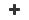
\includegraphics{add3.png}
 & 
Ajoute un nouveau territoire
\\
\hline

\includegraphics{delete4.png}
 & 
Supprime un territoire
\\
\hline\end{tabulary}



\subsection{Ajouter un nouveau territoire}
\label{territories/territorieslist:ajouter-un-nouveau-territoire}
Pour ajouter un nouveau territoire, veuillez cliquer sur l'icone
correspondante dans la barre d'outils du panneau de gauche. Cela
affiche le formulaire d'ajout de territoire comme illustré ci-dessous.

\scalebox{0.800000}{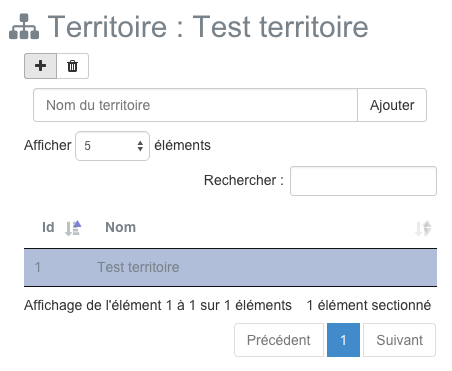
\includegraphics{add-territory-window.png}}

Veuillez spécifier un nom dans la zone de texte prévue à cet effet
puis cliquer sur le bouton ``Ajouter''. Cela entraine la disparution du
formulaire, l'ajout du territoire à l'arbre et le rechargement du
panneau de la {\hyperref[territories/infopanel::doc]{\emph{\emph{Panneau d'information}}}}, à droite de l'écran.


\subsection{Supprimer un territoire}
\label{territories/territorieslist:supprimer-un-territoire}
Pour supprimer un territoire existant, veuillez cliquer sur le nom du
territoire dans la table, puis sur l'icone de suppression dans la
barre d'outils du panneau de gauche. Cela affiche le formulaire de
suppression de territoire comme illustré ci-dessous.

\scalebox{0.800000}{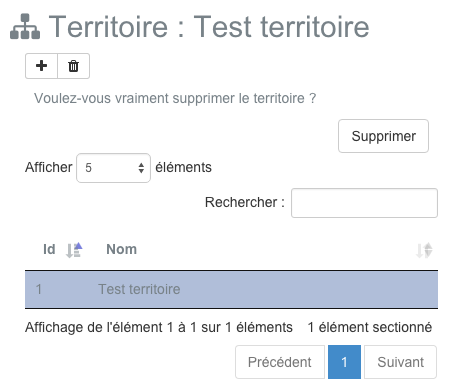
\includegraphics{delete-territory-window.png}}

Cliquez ensuite sur le bouton ``Supprimer''. Cela entraine la
disparution du formulaire et la suppression du territoire de l'arbre.

\begin{notice}{warning}{Avertissement:}
La suppression d'un territoire est permanente et irréversible
\end{notice}


\section{Panneau d'information}
\label{territories/infopanel::doc}\label{territories/infopanel:territories-infopanel}\label{territories/infopanel:panneau-d-information}\setbox0\vbox{
\begin{minipage}{0.95\linewidth}
\textbf{Table des matières}

\medskip

\begin{itemize}
\item {} 
\phantomsection\label{territories/infopanel:id1}{\hyperref[territories/infopanel:panneau-d-information]{\emph{Panneau d'information}}}
\begin{itemize}
\item {} 
\phantomsection\label{territories/infopanel:id2}{\hyperref[territories/infopanel:nom-du-territoire]{\emph{Nom du territoire}}}

\item {} 
\phantomsection\label{territories/infopanel:id3}{\hyperref[territories/infopanel:donnee-geographique]{\emph{Donnée géographique}}}

\item {} 
\phantomsection\label{territories/infopanel:id4}{\hyperref[territories/infopanel:territoire-parent]{\emph{Territoire parent}}}

\item {} 
\phantomsection\label{territories/infopanel:id5}{\hyperref[territories/infopanel:droits-des-groupes]{\emph{Droits des groupes}}}

\end{itemize}

\end{itemize}
\end{minipage}}
\begin{center}\setlength{\fboxsep}{5pt}\shadowbox{\box0}\end{center}

Le panneau d'information des territoires permet de visualiser et d'éditer les propriétés du territoire séléctionné dans le panneau des territoires.

\scalebox{0.800000}{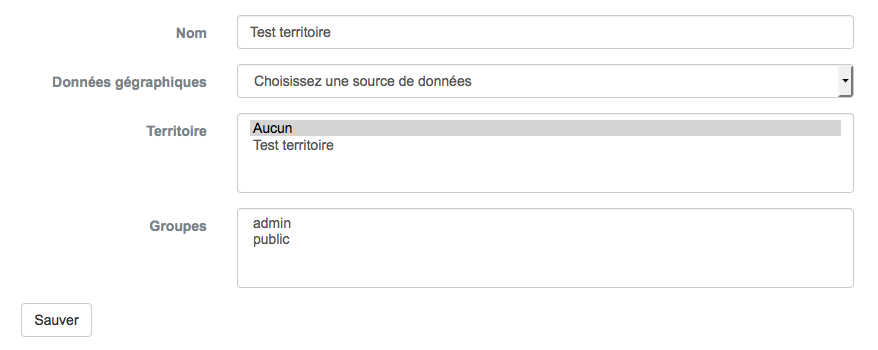
\includegraphics{territory-infopanel-window.png}}


\subsection{Nom du territoire}
\label{territories/infopanel:nom-du-territoire}
Le nom du territoire renseigné doit étre synthétique. La valeur du champs texte est utilisée dans l'interface publique.


\subsection{Donnée géographique}
\label{territories/infopanel:donnee-geographique}
Sélectionnez la table de la base de données que vous souhaitez attribuer au territoire, à l'aide de la liste déroulante prévue à cet effet.


\subsection{Territoire parent}
\label{territories/infopanel:territoire-parent}
Sélectionnez le/les territoires parents avec la liste à choix multiple prévue à cet effet.


\subsection{Droits des groupes}
\label{territories/infopanel:droits-des-groupes}
L'accés au territoire peut étre restreint à certain groupes d'utilisateurs. Cliquez sur le/les groupes ciblés dans la liste à choix multiple prévue à cet effet.

\begin{notice}{note}{Note:}
Cliquez en maintenant la touche Shift enfoncée pour sélectionner plusieurs groupes.
\end{notice}

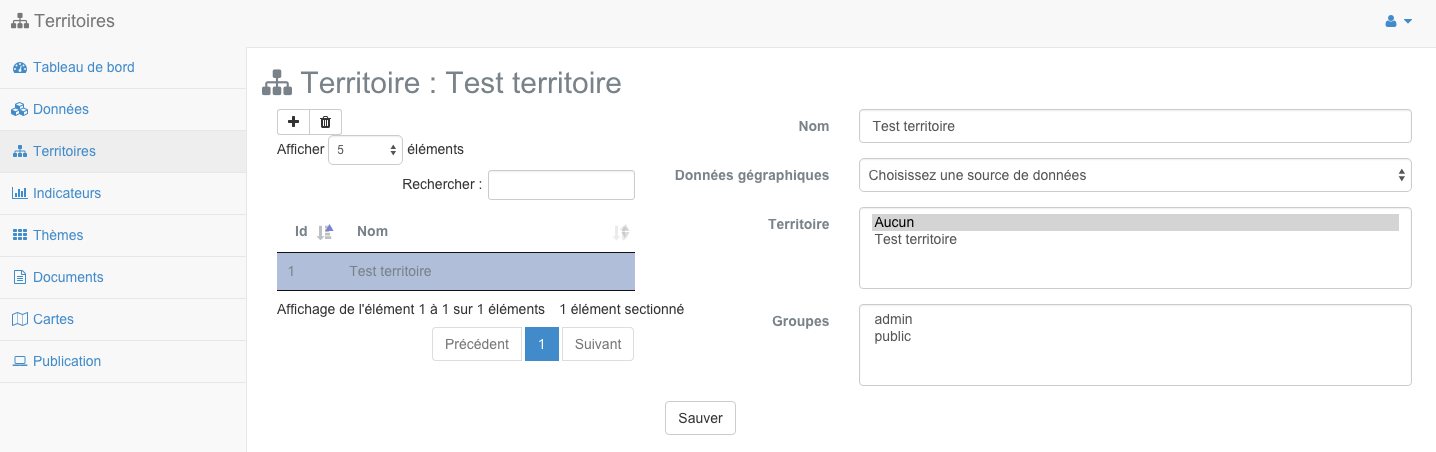
\includegraphics[width=1.000\linewidth]{territory-module-preview.png}


\chapter{Module de gestion des données}
\label{data/index:data}\label{data/index::doc}\label{data/index:module-de-gestion-des-donnees}
Cette section regroupe la documentation relative au module de gestion des données de MapMint.

MapMint utilise la librairie d'abstraction des accès aux données
géographiques \href{http://www.gdal.org}{GDAL}, ainsi le système est en
mesure d'accéder de manière similaire à une base de données, un
répertoire ou des données diffusées via les services de l'\href{http://www.opengeospatial.org}{OGC} (WMS et WFS sont actuellement
supportés). Ainsi, MapMint définit la notion d'\textbf{espaces de stockage}
et de \textbf{source de données}, où un espace de stockage correspond à un
répertoire, une base de données ou encore un serveur fournissant des
services web OGC et, une source de données correspond à un fichier
dans un répertoire, une table géographique de la base de données ou
encore une couche disponible diffusée via un service web OGC.


\section{Espaces de stockage}
\label{data/datastores:datadatastores}\label{data/datastores::doc}\label{data/datastores:espaces-de-stockage}\setbox0\vbox{
\begin{minipage}{0.95\linewidth}
\textbf{Table des matières}

\medskip

\begin{itemize}
\item {} 
\phantomsection\label{data/datastores:id1}{\hyperref[data/datastores:espaces-de-stockage]{\emph{Espaces de stockage}}}
\begin{itemize}
\item {} 
\phantomsection\label{data/datastores:id2}{\hyperref[data/datastores:ajouter-un-espace-de-stockage]{\emph{Ajouter un espace de stockage}}}
\begin{itemize}
\item {} 
\phantomsection\label{data/datastores:id3}{\hyperref[data/datastores:repertoires]{\emph{Répertoires}}}

\item {} 
\phantomsection\label{data/datastores:id4}{\hyperref[data/datastores:base-de-donnees]{\emph{Base de données}}}

\item {} 
\phantomsection\label{data/datastores:id5}{\hyperref[data/datastores:serveurs-ogc]{\emph{Serveurs OGC}}}

\end{itemize}

\item {} 
\phantomsection\label{data/datastores:id6}{\hyperref[data/datastores:acceder-a-un-espace-de-stockage]{\emph{Accéder à un espace de stockage}}}
\begin{itemize}
\item {} 
\phantomsection\label{data/datastores:id7}{\hyperref[data/datastores:barre-d-outils-d-un-espace-de-stockage]{\emph{Barre d'outils d'un espace de stockage}}}

\item {} 
\phantomsection\label{data/datastores:id8}{\hyperref[data/datastores:creer-une-mosaique-d-images]{\emph{Créer une mosaïque d'images}}}

\item {} 
\phantomsection\label{data/datastores:id9}{\hyperref[data/datastores:envoyer-une-source-de-donnees-dans-un-espace-de-stockage]{\emph{Envoyer une source de données dans un espace de stockage}}}

\item {} 
\phantomsection\label{data/datastores:id10}{\hyperref[data/datastores:creer-un-index-de-tuiles-dans-un-espace-de-stockage]{\emph{Créer un index de tuiles dans un espace de stockage}}}

\item {} 
\phantomsection\label{data/datastores:id11}{\hyperref[data/datastores:gestion-des-droits-d-acces-d-un-espace-de-stockage]{\emph{Gestion des droits d'accés d'un espace de stockage}}}

\item {} 
\phantomsection\label{data/datastores:id12}{\hyperref[data/datastores:parametrage-d-un-espace-de-stockage]{\emph{Paramétrage d'un espace de stockage}}}

\item {} 
\phantomsection\label{data/datastores:id13}{\hyperref[data/datastores:supprimer-un-espace-de-stockage]{\emph{Supprimer un espace de stockage}}}

\item {} 
\phantomsection\label{data/datastores:id14}{\hyperref[data/datastores:rafraichir-un-espace-de-stockage]{\emph{Rafraichir un espace de stockage}}}

\end{itemize}

\end{itemize}

\end{itemize}
\end{minipage}}
\begin{center}\setlength{\fboxsep}{5pt}\shadowbox{\box0}\end{center}

Un espace de stockage contient des sources de données, locales ou
distantes. Il est définit par un nom (sans accents, espace ou
caractères spéciaux), ainsi que par différents paramètres selon son
type. Il existe quatre types d'espaces de stockage dans MapMint:

\begin{tabulary}{\linewidth}{|L|L|L|}
\hline

\textbf{Icône}
 & 
\textbf{Type}
 & 
\textbf{Action}
\\
\hline

\includegraphics{database.png}
 & 
Base de données
 & 
Ajout d'une connexion à une base de données
\\
\hline

\includegraphics{directory.png}
 & 
Répertoire
 & 
Ajout d'un répertoire de données
\\
\hline

\includegraphics{ogcserver.png}
 & 
Serveur OGC
 & 
Ajout d'un serveur OGC externe
\\
\hline\end{tabulary}


\begin{notice}{warning}{Avertissement:}
Le nom d'un espace de stockage ne doit contenir ni \emph{espace}, \emph{accent} ou \emph{caractères spéciaux}
\end{notice}


\subsection{Ajouter un espace de stockage}
\label{data/datastores:ajouter-un-espace-de-stockage}\label{data/datastores:datadatastores-add}

\subsubsection{Répertoires}
\label{data/datastores:repertoires}
Un espace de stockage de type répertoire permet d'établir un lien
symbolique vers un répertoire de données du serveur FTP. Cliquez sur
l'icône ``Ajouter un répertoire'' se trouvant dans la barre
d'outils. Cela entraine l'affichage du formulaire d'ajout d'un
répertoire.

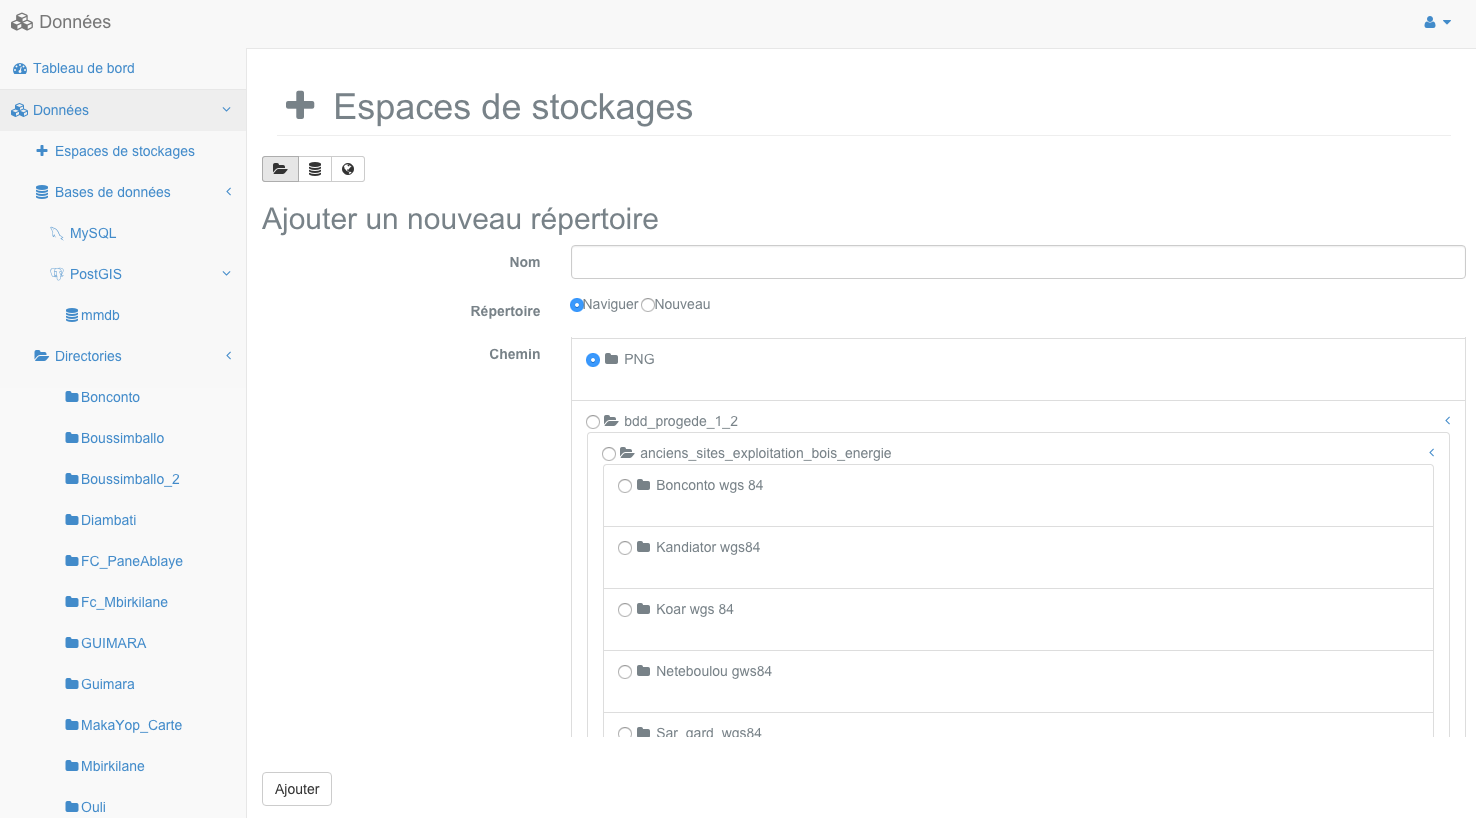
\includegraphics[width=1.000\linewidth]{add-directory-window.png}

Renseignez le nom de l'espace de stockage puis sélectionnez un
répertoire du serveur dans l'arbre des répertoires (arborescence du
repértoire /data de l'instance MapMint). Vous avez la possibilité de
créer un répertoire vide sur le serveur FTP, en choisissant l'option
``nouveau'', vous devez alors aussi donner un nom au répertoire à
créer.

\begin{notice}{warning}{Avertissement:}
Le répertoire ciblé ne doit pas contenir de sous-répertoires.
\end{notice}

\begin{notice}{warning}{Avertissement:}
Le repertoire ciblé doit contenir uniquement des formats de données supportés par MapMint.
\end{notice}

Cela entraîne la fermeture de la fenêtre et l'ajout du nouvel espace de stockage dans l'abre de gauche, dans la section Répertoires.

\begin{notice}{note}{Note:}
Une fois l'espace de stockage crée, procéder à un clic droit sur ce dernier et cliquer sur ``Rafraichir''.
\end{notice}

Le clic sur l'espace de stockage entraine l'affichage des sources de données qu'il contient dans le panneau des {\hyperref[data/datasources::doc]{\emph{\emph{Sources de données}}}}.


\subsubsection{Base de données}
\label{data/datastores:base-de-donnees}
Un espace de stockage de type base de données permet d'établir une
connexion avec une base de données PostgreSQL ou MySQL. Cliquez sur
l'icône ``Ajouter une base de données'' se trouvant dans la barre
d'outils en haut du panneau des espaces de stockages. Cela entraine
l'affichage du formulaire d'ajout d'une connexion à une base de données
comme illustré ci-dessous.

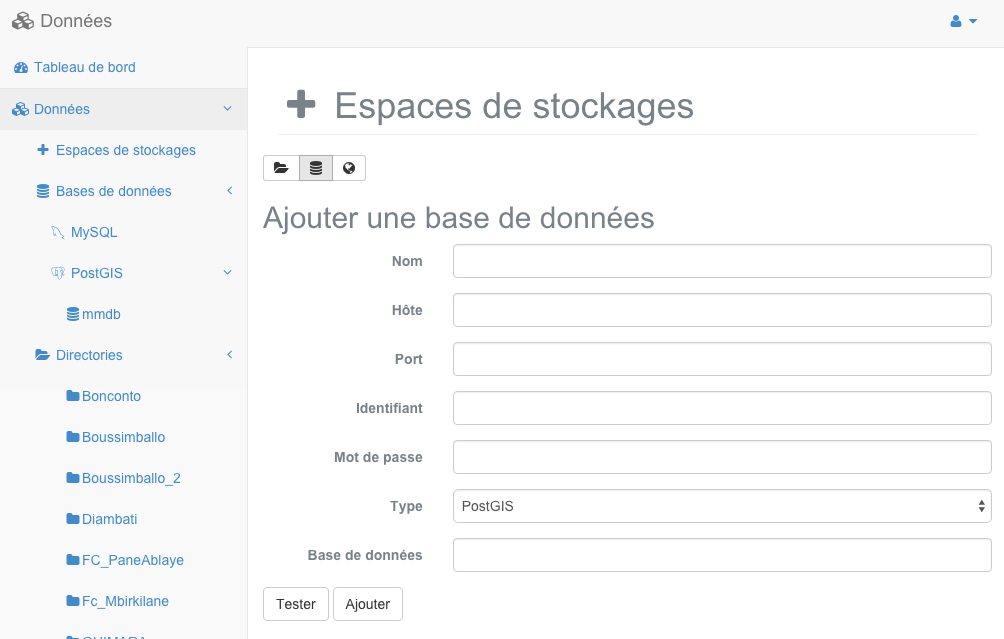
\includegraphics[width=1.000\linewidth]{add-database-window.png}

Renseignez tous les champs puis cliquez sur le bouton ``Tester''.

Si le test renvoie un message de succès, vous pouvez alors cliquer sur le bouton ``Ajouter''. Cela entraîne la fermeture de la fenêtre et l'ajout du nouvel espace de stockage dans l'abre de gauche, dans la section PostGIS ou MySQL.

\begin{notice}{note}{Note:}
Une fois l'espace de stockage crée, cliquez sur ce dernier dans le
menu de gauche pour le voir se charger dans la partie de droite
comme présenté sur la capture d'écran précédente.
\end{notice}

Le clic sur l'espace de stockage entraine son affichage dans la
partie de droite.


\subsubsection{Serveurs OGC}
\label{data/datastores:serveurs-ogc}
Un espace de stockage de type serveur OGC permet d'établir une
connexion à un serveur WMS ou WFS externe. Cliquez sur l'icône
``Ajouter un serveur OGC'' se trouvant dans la barre d'outils, cela
entraine l'affichage du formulaire d'ajout d'un serveur OGC.

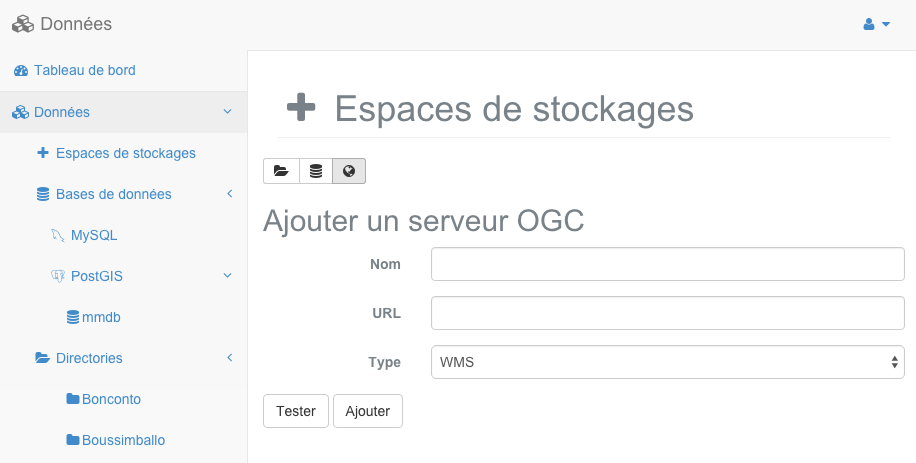
\includegraphics[width=1.000\linewidth]{add-ogcserver-window.png}

Renseignez le nom de l'espace de stockage, l'URL du serveur OGC ciblé
ainsi que le protocole à utiliser (WMS ou WFS), puis cliquez sur le
bouton ``Tester''.

Si le test renvoie un message de succès, vous pouvez alors cliquer sur le bouton ``Ajouter''. Cela entraîne la fermeture de la fenêtre et l'ajout du nouvel espace de stockage dans l'arbre de gauche, dans la section Serveur WFS.

Le clic sur l'espace de stockage entraine l'affichage des couches OGC du serveur externe.


\subsection{Accéder à un espace de stockage}
\label{data/datastores:acceder-a-un-espace-de-stockage}
Lorsque vous cliquez sur l'espace de stockage cela entraine son
affichage comme illstré ci-dessous.

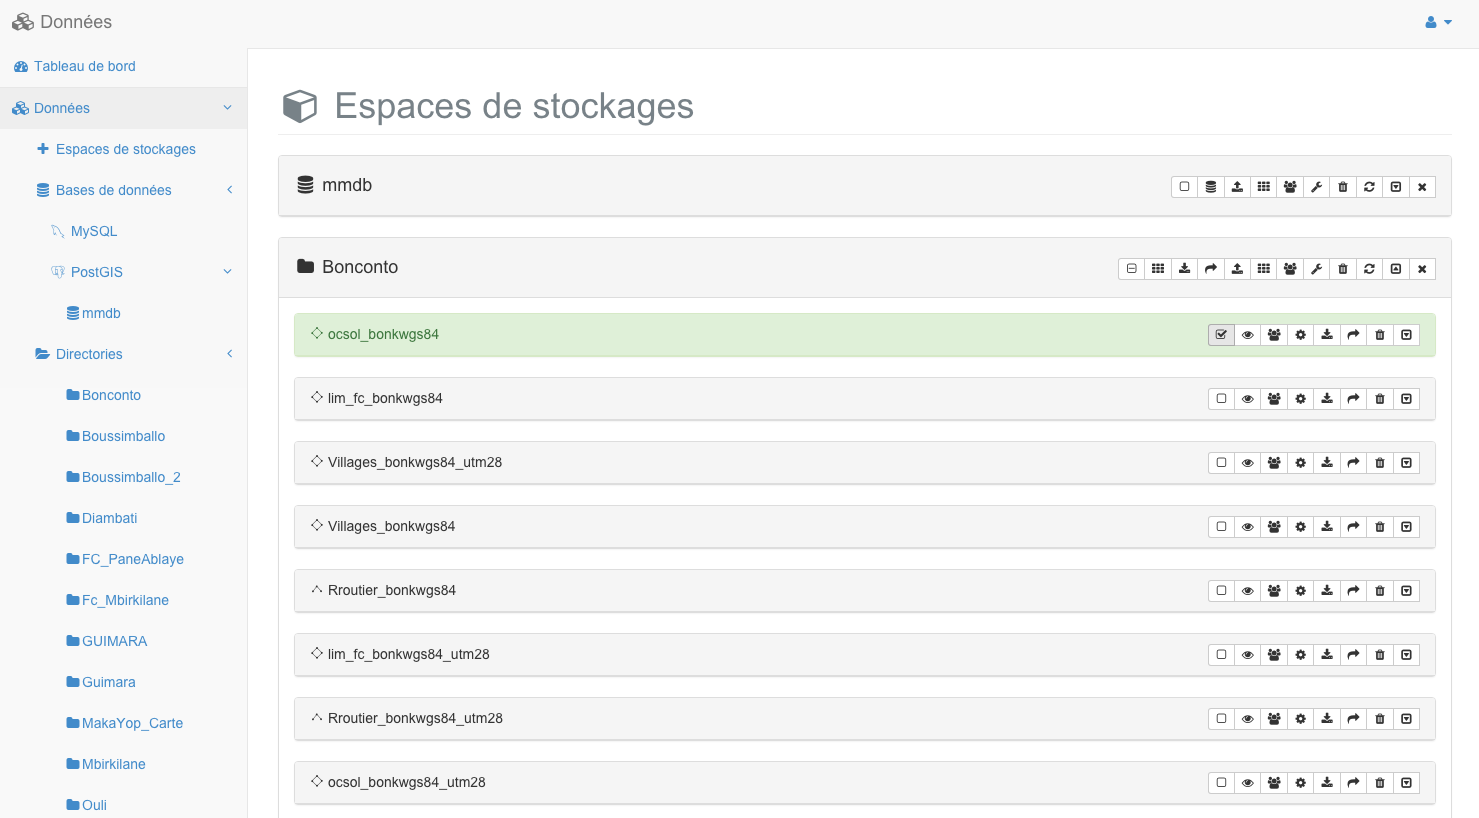
\includegraphics[width=1.000\linewidth]{data-store-preview.png}

Les espaces de stockage offrent des fonctions spécifiques suivant leur
type, l'ensemble des boutons de la barre d'outils correspondante à un
espace de stockagre est présenté ci-dessous. Pour chaque bouton, le
type d'espace de stockage depuis lequel la fonctionnalité est
accessible est aussi mise en évidence.


\subsubsection{Barre d'outils d'un espace de stockage}
\label{data/datastores:barre-d-outils-d-un-espace-de-stockage}
\begin{tabulary}{\linewidth}{|L|L|L|}
\hline

\textbf{Icône}
 & 
\textbf{Accessible}
 & 
\textbf{Action}
\\
\hline

\includegraphics{select.png}
 & 
Tous
 & 
Selectionnez toutes les sources de données contenues
\\
\hline

\includegraphics{tile.png}
 & 
Répertoire
 & 
Créer une mosaïc d'images (requiert une source de données image sélectionnée)
\\
\hline

\includegraphics{download.png}
 & 
Répertoire
 & 
Télécharge les sources de données sélectionnées (requiert une source de données image sélectionnée)
\\
\hline

\includegraphics{share.png}
 & 
Tous
 & 
Ouvrir les sources de données selectionnées dans le {\hyperref[maps/index:maps]{\emph{Module de création de cartes}}} (requiert une source de données sélectionnée)
\\
\hline
\includegraphics{database.png}
 & 
Base de données
 & 
Accéder à la base de données
\\
\hline
\includegraphics{upload.png}
 & 
Répertoire
 & 
Envoyez une source de données dans l'espace de stockage du serveur
\\
\hline
\includegraphics{tile.png}
 & 
Répertoire
 & 
Créer un index de tuiles dans l'espace de stockage
\\
\hline
\includegraphics{privileges.png}
 & 
Toute
 & 
Gestion des droits d'accés d'un espace de stockage
\\
\hline
\includegraphics{configuration.png}
 & 
Tout
 & 
Paramétrage de l'espace de stockage
\\
\hline
\includegraphics{delete.png}
 & 
Tous
 & 
Supprimer l'espace de stockage
\\
\hline
\includegraphics{refresh.png}
 & 
Tous
 & 
Rafraichir l'espace de stockage
\\
\hline
\includegraphics{toggle1.png}
 & 
Tous
 & 
Afficher / masquer l'espace de stockage
\\
\hline
\includegraphics{close.png}
 & 
Tous
 & 
Fermer l'espace de stockage
\\
\hline\end{tabulary}



\subsubsection{Créer une mosaïque d'images}
\label{data/datastores:creer-une-mosaique-d-images}
La création d'une mosaïque d'images permet
de fusionner plusieurs sources de données images en une seule.

Lorsque vous cliquez sur le boutton ``Créer une mozaïc d'images'' le
formulaire présenté ci-desous s'affiche. Une fois que vous avez
renseigné le nom de la mosaïque à créer, cliquez sur le bouton
``Mosaïque'' pour le générer.

\begin{notice}{warning}{Avertissement:}
Cette opération peut prendre du temps suivant les sources de
données images sélectionnées.
\end{notice}

\includegraphics[width=1.000\linewidth]{data-store-mozaic.png}


\subsubsection{Envoyer une source de données dans un espace de stockage}
\label{data/datastores:envoyer-une-source-de-donnees-dans-un-espace-de-stockage}
Vous pouvez utiliser le panneau d'un espace de stockage pour y envoyer
un fichier de données géographique que vous avez sur votre machine
locale. Ceci se fait à l'aide du formulaire présenté ci-dessous.

Vous pouvez alors cliquer sur le boutton ``Parcourir'' afin d'ajouter
vos fichiers à la liste des fichiers à envoyer.

\begin{notice}{warning}{Avertissement:}
Bien que la fonctionnalité d'envoi de sources de données soit
disponible sur la plateforme MapMint, elle ne devrait être
utilisée que pour des sources de données ne dépassant pas 10Mo.
\end{notice}

\includegraphics[width=1.000\linewidth]{data-store-upload.png}


\subsubsection{Créer un index de tuiles dans un espace de stockage}
\label{data/datastores:creer-un-index-de-tuiles-dans-un-espace-de-stockage}
Lorsque que l'on souhaite publier des sources de données images de
type photo aériennes par exemple, il est nécessaire d'utiliser un
index de tuiles. Un index de tuiles est une source de données vecteurs
(de type polygone) où chaque polygon représente la zone géographique
couverte par une source de données images (une photos aérienne par
exemple) et a une seule propriété qui est le chemin complet vers le
fichier image.

Pour créer un index de tuiles, vous devez placer un répertoire
contenant l'ensemble des photos à partir desquelles vous souhaitez
créer un index de tuiles. Une fois ceci fait, vous pouvez cliquer sur
le boutton ``Créer un index de tuiles'' de l'espace de stockage dans
lequel vous souhaitez le stocker, le formulaire présenté ci-dessous
apparait. Sélectionnez le SRS de l'index à créer, saisissez
l'extension des fichiers à utiliser (tif par exemple) puis cochez le
répertoire stockant vos photos, cliquez ensuite sur le boutton ``Index
de tuiles'' pour générer l'index de tuiles.

\includegraphics[width=1.000\linewidth]{data-tileindex.png}


\subsubsection{Gestion des droits d'accés d'un espace de stockage}
\label{data/datastores:gestion-des-droits-d-acces-d-un-espace-de-stockage}
Une source de données est accessible à tous les groupes d'utilisateurs
par défaut. Pour modifier les permissions l'accès à une couche,
veuillez cliquer sur l'icone correspondante dans la
{\hyperref[data/datasources:datasource-table-label]{\emph{Barre d'outils des sources de données}}}. Celà entraîne l'affichage du formulaire
de gestion de droits d'accès, illustré ci-dessous.

\includegraphics[width=1.000\linewidth]{data-privileges.png}

Les droits que vous pouvez affecter à un groupe d'utilisateurs sont
listés dans la table suivante.

\begin{tabulary}{\linewidth}{|L|L|}
\hline

\textbf{Valeur}
 & 
\textbf{Définition}
\\
\hline
r
 & 
Le groupe d'utilisateurs à accès à l'espace de stockage en lecture
\\
\hline
w
 & 
Le groupe d'utilisateurs à accès à l'espace de stockage en écriture
\\
\hline
x
 & 
Le groupe d'utilisateurs à le droit d'exécuter des services dans l'espace de stockage
\\
\hline\end{tabulary}


Ajoutez un ou plusieur groupes avec le bouton ``Ajouter'', cela entraine
l'ajout de listes déroulantes dans la fenêtre. Ajustez les valeurs
\textbf{r}, \textbf{w} et \textbf{x} puis cliquer sur le bouton ``Valider''. Le
formulaire disparait et l'enregistrement des modifications est réalisé.

Si vous cliquez sur le boutton ``Supprimer'' vous pouvez supprimer la
dernière ligne de définition de privilèges d'accès.

Pour voir le droit de lister le contenu d'un espace de stockage un
groupe d'utilisateurs doit avoir les droits \textbf{r} et \textbf{x}. Pour
pouvoir créer de nouvelles sources de données dans l'espace de
stockage, un groupe doit avoir le droit \textbf{w}.


\subsubsection{Paramétrage d'un espace de stockage}
\label{data/datastores:parametrage-d-un-espace-de-stockage}
Le formulaire de paramétrage d'un espace de stockage et équivalent au
formulaire d'ajout spécifique au type d'espace de stockage vu
{\hyperref[data/datastores:datadatastores-add]{\emph{précédemment}}}.


\subsubsection{Supprimer un espace de stockage}
\label{data/datastores:supprimer-un-espace-de-stockage}
Si vous cliquez sur le boutton ``Supprimer l’espace de stockage'', une
fenêtre apparait vous invitant à confirmer votre volonté de supprimer
un espace de stockage. La suppression d'un espace de stockage peut
entrainer des pertes de données graves et impliquer que l'application
grand publique devienne instable du fait de l'indisponibilité de
certaines sources de données nécessaires. Il est donc impératif de
s'assurer qu'aucun projet ne dépend de données présentes dans l'espace
de stockage que vous souhaitez supprimer avant de le faire. Si vous
souhaitez vraiment supprimer un espace de stockage, cliquez alors sur
le bouton ``Oui'' de la fenêtre vous informant des implications
de la suppression.


\subsubsection{Rafraichir un espace de stockage}
\label{data/datastores:rafraichir-un-espace-de-stockage}
Lors du premier accès à un espace de stockage, MapMint crée un fichier
Mapfile spécifique à MapServer qui permet la diffusion des sources de
données contenues. Une fois ce fichier créé, il n'est plus
modifié. Cela implique que si vous avez ajouté, supprimé ou créée une
nouvelle source de données dans un espace de stockage, vous devrez
utilisez le boutton de rafraichissement permettant d'obtenir une liste
exhaustive des sources de données contenues dans un espace de
stockage. Lorsque vous cliquez sur le boutton de rafraichissement, le
contenu de l'espace de stockage est mis à jour.


\section{Sources de données}
\label{data/datasources:data-datasources}\label{data/datasources::doc}\label{data/datasources:sources-de-donnees}\setbox0\vbox{
\begin{minipage}{0.95\linewidth}
\textbf{Table des matières}

\medskip

\begin{itemize}
\item {} 
\phantomsection\label{data/datasources:id2}{\hyperref[data/datasources:sources-de-donnees]{\emph{Sources de données}}}
\begin{itemize}
\item {} 
\phantomsection\label{data/datasources:id3}{\hyperref[data/datasources:donnees-vectorielles]{\emph{Données vectorielles}}}
\begin{itemize}
\item {} 
\phantomsection\label{data/datasources:id4}{\hyperref[data/datasources:formats-supportes]{\emph{Formats supportés}}}

\item {} 
\phantomsection\label{data/datasources:id5}{\hyperref[data/datasources:consulter-la-table]{\emph{Consulter la table}}}

\item {} 
\phantomsection\label{data/datasources:id6}{\hyperref[data/datasources:definir-l-encodage-des-caracteres-de-la-table]{\emph{Définir l'encodage des caractères de la table}}}

\end{itemize}

\item {} 
\phantomsection\label{data/datasources:id7}{\hyperref[data/datasources:donnees-matricielles]{\emph{Données matricielles}}}
\begin{itemize}
\item {} 
\phantomsection\label{data/datasources:id8}{\hyperref[data/datasources:id1]{\emph{Formats supportés}}}

\item {} 
\phantomsection\label{data/datasources:id9}{\hyperref[data/datasources:consulter-l-histogramme]{\emph{Consulter l'histogramme}}}

\end{itemize}

\item {} 
\phantomsection\label{data/datasources:id10}{\hyperref[data/datasources:barre-d-outils-des-sources-de-donnees]{\emph{Barre d'outils des sources de données}}}
\begin{itemize}
\item {} 
\phantomsection\label{data/datasources:id11}{\hyperref[data/datasources:droits-d-acces]{\emph{Droits d'accès}}}

\item {} 
\phantomsection\label{data/datasources:id12}{\hyperref[data/datasources:convertir-une-source-de-donnees]{\emph{Convertir une source de données}}}

\item {} 
\phantomsection\label{data/datasources:id13}{\hyperref[data/datasources:telechargement]{\emph{Téléchargement}}}

\item {} 
\phantomsection\label{data/datasources:id14}{\hyperref[data/datasources:previsualisation]{\emph{Prévisualisation}}}

\item {} 
\phantomsection\label{data/datasources:id15}{\hyperref[data/datasources:suppression]{\emph{Suppression}}}

\item {} 
\phantomsection\label{data/datasources:id16}{\hyperref[data/datasources:ouverture]{\emph{Ouverture}}}

\end{itemize}

\end{itemize}

\end{itemize}
\end{minipage}}
\begin{center}\setlength{\fboxsep}{5pt}\shadowbox{\box0}\end{center}

Une source de données est constituée d'une ou plusieurs informations à références spatiales, contenues par l'un des {\hyperref[data/datastores::doc]{\emph{\emph{Espaces de stockage}}}} disponibles. MapMint supporte plusieurs types de sources de données décrites dans cette section.

Les pictogrammes utilisés pour illustrer le type d'une source de
données sont présentés dans la table suivante.

\begin{tabulary}{\linewidth}{|L|L|}
\hline

\textbf{Icône}
 & 
\textbf{Type}
\\
\hline
\includegraphics{data-vector-point-icon.png}
 & 
Source de données vectorielles de type Point
\\
\hline
\includegraphics{data-vector-line-icon.png}
 & 
Source de données vectorielles de type Ligne
\\
\hline
\includegraphics{data-vector-polygon-icon.png}
 & 
Source de données vectorielles de type Polygone
\\
\hline
\includegraphics{data-raster-icon.png}
 & 
Source de données matricielles
\\
\hline\end{tabulary}



\subsection{Données vectorielles}
\label{data/datasources:donnees-vectorielles}

\subsubsection{Formats supportés}
\label{data/datasources:formats-supportes}
MapMint supporte les formats de données vectorielles listés ci-dessous.

\begin{tabulary}{\linewidth}{|L|L|L|}
\hline

\textbf{Format}
 & 
\textbf{Code}
 & 
\textbf{Fichiers nécessaires}
\\
\hline
Comma Separated Value
 & 
CSV
 & 
csv
\\
\hline
ESRI Shapefile
 & 
SHP
 & 
shp,dbf,shx,prj
\\
\hline
GPX
 & 
GPX
 & 
gpx
\\
\hline
Mapinfo
 & 
MIF
 & 
mif
\\
\hline
KML
 & 
KML
 & 
kml
\\
\hline
PostgreSQL/PostGIS
 & 
PostGIS
 & 
connexion PostGIS
\\
\hline
Web Feature Service
 & 
WFS
 & 
connexion WFS
\\
\hline\end{tabulary}


\begin{notice}{note}{Note:}
D'autre \href{http://www.gdal.org/ogr/ogr\_formats.html}{formats} supportés par la libraire \href{http://www.gdal.org/ogr}{OGR} peuvent également être utilisés avec MapMint.
\end{notice}


\subsubsection{Consulter la table}
\label{data/datasources:consulter-la-table}
Pour consulter la table d'une source de données, veuillez cliquer sur
l'icône ``flèche'' à droite de la {\hyperref[data/datasources:datasource-table-label]{\emph{Barre d'outils des sources de données}}}. Cela
entraine l'éffichage de la table de données. Un exemple de cette
table est présenté ci-après.

\includegraphics[width=1.000\linewidth]{view-datasource-table.png}

Une fois la table affichée, et si celle-ci contient un nombre
d'entités suffisant, il est possible de naviguer dans les différentes
pages de la table à l'aide des bouttons ``Précédent'' et ``Suivant'' de
navigation affichée en bas de la table ou en cliquant directement sur
le numéro de la page souhaitée.

Dans le cas où le contenu de la table correspondante à votre source de
données ne serait pas affiché correctement, consulter la section
\DUspan{xref,std,std-ref}{data-datasources-encoding}. vous devrez alors définir
l'encodage de votre source données, en utilisant le champs texte prévu
à cet effet puis en cliquant sur le bouton ``Définir''.

\begin{notice}{note}{Note:}
La liste déroulante en haut à gauche de la table vous permet d'afficher 10, 15, 20, 25 ou 30 entités par page
\end{notice}

\begin{notice}{note}{Note:}
Le clic sur un titre d'une colone trie les valeurs par ordre croissant/décroissant ou par ordre alphabétique.
\end{notice}


\subsubsection{Définir l'encodage des caractères de la table}
\label{data/datasources:definir-l-encodage-des-caracteres-de-la-table}
MapMint utilise l'encodage UTF-8 par défaut pour afficher les tables des sources de données. Il est toutefois fréquent que des données encodées dans un autre système soient chargées dans le module de gestion des données. Dans ce cas, il est possible d'assigner un système d'encodage différent dans le champs texte prévu à cet effet, à droite de la barre de navigation.

Veuillez y entrer le code de l'encodage désiré, puis cliquez sur l'icône ``Rafraichir'' de la barre d'outil. Cela entrâine le rechargement de la table et son affichage dans l'encodage souhaité.

Des exemples d'encodage de caractère sont listés ci-dessous à titre informatif:

\begin{tabulary}{\linewidth}{|L|L|}
\hline

\textbf{Code}
 & 
\textbf{Description}
\\
\hline
utf-8
 & 
Ensemble des caractères internationaux d'unicode compatible avec la norme ASCII (anglais)
\\
\hline
iso-8859-1
 & 
Alphabet latin numéro 1 contenant 191 caractères de l'alphabet latin
\\
\hline
iscii
 & 
Alphasyllabaires utilisés en Inde, au Sri Lanka et au Bangladesh
\\
\hline
viscii
 & 
Alphabet latin moderne du vietnamien
\\
\hline
shift-jis
 & 
Syllabaires et écriture sinographique traditionnelle des langues japonaises
\\
\hline\end{tabulary}


\begin{notice}{note}{Note:}
Obtenez plus d'informatons sur le codage des caractères sur \href{http://fr.wikipedia.org/wiki/Codage\_des\_caract\%C3\%A8res}{Wikipédia}
\end{notice}


\subsection{Données matricielles}
\label{data/datasources:donnees-matricielles}

\subsubsection{Formats supportés}
\label{data/datasources:id1}
apMint supporte les formats de données matricielles listés ci-dessous.

\begin{tabulary}{\linewidth}{|L|L|L|}
\hline

\textbf{Format}
 & 
\textbf{Code}
 & 
\textbf{Fichiers nécessaires}
\\
\hline
Arc/Info ASCII Grid
 & 
AAIGrid
 & 
asc
\\
\hline
GeoTiff
 & 
GTiff
 & 
tif
\\
\hline
JPEG
 & 
JPEG
 & 
jpg
\\
\hline\end{tabulary}


\begin{notice}{note}{Note:}
D'autre \href{http://www.gdal.org/formats\_list.html}{formats} supportés par la libraire \href{http://www.gdal.org}{GDAL} peuvent également être utilisés avec MapMint.
\end{notice}


\subsubsection{Consulter l'histogramme}
\label{data/datasources:consulter-l-histogramme}
Pour consulter l'histogramme d'une source de données, veuillez cliquer sur l'icône ``flèche'' à droite de la {\hyperref[data/datasources:datasource-table-label]{\emph{Barre d'outils des sources de données}}}. Cela entraîne le depliement de l'histogramme, comme illustré ci-après.

\includegraphics[width=1.000\linewidth]{view-datasource-histogram.png}

L'histogramme de la source de données vous permet de consulter la distribution de sa/ses bande(s) dans la matrice de pixel.

\begin{notice}{note}{Note:}
Il est possible de zoomer dans l'histogramme en maintenant votre curseur et en desssinant un rectangle
\end{notice}


\subsection{Barre d'outils des sources de données}
\label{data/datasources:barre-d-outils-des-sources-de-donnees}\label{data/datasources:datasource-table-label}
\begin{tabulary}{\linewidth}{|L|L|}
\hline

\textbf{Icône}
 & 
\textbf{Action}
\\
\hline
\includegraphics{privileges.png}
 & 
Définir les permissions d'accès d'une source de données
\\
\hline
\includegraphics{process1.png}
 & 
Convertir une source de données
\\
\hline
\includegraphics{download.png}
 & 
Télécharger une source de données
\\
\hline
\includegraphics{preview.png}
 & 
Prévisualiser une source de données
\\
\hline
\includegraphics{share.png}
 & 
Ouvrir une source de données dans le module de création de cartes
\\
\hline
\includegraphics{delete.png}
 & 
Supprimer une source de données
\\
\hline\end{tabulary}



\subsubsection{Droits d'accès}
\label{data/datasources:droits-d-acces}
Une source de données est accessible à tous les groupes d'utilisateurs par défaut. Pour modifier les permissions l'accès à une couche, veuillez cliquer sur l'icone correspondant dans la {\hyperref[data/datasources:datasource-table-label]{\emph{Barre d'outils des sources de données}}}. Celà entraîne l'ouverture de la fenêtre des droits d'accès, illustrée ci-dessous:

\includegraphics[width=1.000\linewidth]{data-privileges.png}

\begin{tabulary}{\linewidth}{|L|L|}
\hline

\textbf{Valeur}
 & 
\textbf{Définition}
\\
\hline
r
 & 
Le groupe d'utilisateur à accès à la couche en lecture
\\
\hline
w
 & 
Le groupe d'utilisateur à accès à la couche en écriture
\\
\hline
x
 & 
Le groupe d'utilisateur à accès ...
\\
\hline\end{tabulary}


Ajoutez un ou plusieur groupes avec le boutton ``Ajouter'', cela entraine l'ajout de listes déroulantes dans la fenêtre. Ajustez les valeurs \textbf{r}, \textbf{w} et \textbf{x} puis cliquer sur le bouton ``Valider''. La fenêtre se ferme et l'enregistrement des modifications est stipulé en haut de votre écran dans un bandeau de couleur verte.


\subsubsection{Convertir une source de données}
\label{data/datasources:convertir-une-source-de-donnees}
La conversion de données est traitée dans la partie : {\hyperref[data/processing:data-processing]{\emph{Géotraitements}}}.


\subsubsection{Téléchargement}
\label{data/datasources:telechargement}
Pour télécharger une source de données sur votre ordinateur, il suffit de cliquer sur l'icône correspondante dans la {\hyperref[data/datasources:datasource-table-label]{\emph{Barre d'outils des sources de données}}}. Cela engendre le téléchargement direct de la donnée, archivée dans un fichier .zip


\subsubsection{Prévisualisation}
\label{data/datasources:previsualisation}
Pour prévisualiser une source de données, veuillez cliquer sur l'icône
correspondante dans la {\hyperref[data/datasources:datasource-table-label]{\emph{Barre d'outils des sources de données}}}, cela affiche une
bulle de prévisualisation comme illustré ci-dessous.

\begin{tabulary}{\linewidth}{|L|L|}
\hline

\textbf{Source de données vecteur}
 & 
\textbf{Source de données raster}
\\
\hline
\includegraphics[width=1.000\linewidth]{preview-vector-window.png}
 & 
\includegraphics[width=1.000\linewidth]{preview-raster-window.png}
\\
\hline\end{tabulary}


\begin{notice}{note}{Note:}
Les sources de données vecteur sont prévisualisées avec un style par défaut (remplissage violet et bordure gris foncé)
\end{notice}

\begin{notice}{warning}{Avertissement:}
Les sources de données de type WMS externes ne disposent pas de la fonctionnalité de prévisualisation
\end{notice}


\subsubsection{Suppression}
\label{data/datasources:suppression}
Pour supprimer une source de données, veuillez cliquer sur l'icône correspondante dans la {\hyperref[data/datasources:datasource-table-label]{\emph{Barre d'outils des sources de données}}}. Cela ouvre la fenêtre de suppression illustrée ci-après.

\includegraphics[width=1.000\linewidth]{delete-datasource-window.png}

Cliquez sur le bouton ``Supprimer'' pour supprimer la donnée. La fenêtre se ferme et la suppression de la source de données est stipulé en haut de votre écran dans un bandeau de couleur verte.

\begin{notice}{warning}{Avertissement:}
L'utilisation de cette fonctionnalité supprime la source de données de l'espace de stockage et supprime le jeux de données physiquement sur le serveur. Cette action est permanente et irréversible.
\end{notice}


\subsubsection{Ouverture}
\label{data/datasources:ouverture}
Pour ouvrir une source de données dans le {\hyperref[maps/index::doc]{\emph{\emph{Module de création de cartes}}}}, veuillez cliquer sur l'icône correspondante dans la {\hyperref[data/datasources:datasource-table-label]{\emph{Barre d'outils des sources de données}}}. Cela entraine l'ouverture de la source de données dans le {\hyperref[maps/index::doc]{\emph{\emph{Module de création de cartes}}}}. La source de données est ajouté à la racine de l'arbre de couches, dans un projet \emph{Untitled\_0} et représentée avec le style par défaut.

\begin{notice}{note}{Note:}
Une fois la source de données chargée, il est conseillé d'enregistrer le projet \emph{Untitled\_0} sous un nom adéquat
\end{notice}


\section{Géotraitements}
\label{data/processing:data-processing}\label{data/processing::doc}\label{data/processing:geotraitements}\setbox0\vbox{
\begin{minipage}{0.95\linewidth}
\textbf{Table des matières}

\medskip

\begin{itemize}
\item {} 
\phantomsection\label{data/processing:id1}{\hyperref[data/processing:geotraitements]{\emph{Géotraitements}}}
\begin{itemize}
\item {} 
\phantomsection\label{data/processing:id2}{\hyperref[data/processing:convertisseur-de-sources-de-donnees-vectorielles]{\emph{Convertisseur de sources de données vectorielles}}}

\item {} 
\phantomsection\label{data/processing:id3}{\hyperref[data/processing:utilitaire-de-traitements-des-sources-de-donnees-matricielles]{\emph{Utilitaire de traitements des sources de données matricielles}}}

\end{itemize}

\end{itemize}
\end{minipage}}
\begin{center}\setlength{\fboxsep}{5pt}\shadowbox{\box0}\end{center}

Les fonctionnalités de géotraitement de MapMint permettent à
l'utilisateur de créer de nouvelles {\hyperref[data/datasources::doc]{\emph{\emph{Sources de données}}}} en utilisant
celles déja disponibles dans le {\hyperref[data/index::doc]{\emph{\emph{Module de gestion des données}}}}.


\subsection{Convertisseur de sources de données vectorielles}
\label{data/processing:convertisseur-de-sources-de-donnees-vectorielles}
Le convertisseur de données vectorielles fournit une interface
utilisateur à l'outil en ligne de commande \href{http://www.gdal.org/ogr2ogr.html}{ogr2ogr} de la librairie \href{http://www.gdal.org/ogr/}{OGR}. Il permet de convertir et de reprojeter
une source de données vectorielles.

Pour y accéder, veuillez cliquer sur l'icône correspondante dans la
barre d'outils des {\hyperref[data/datasources::doc]{\emph{\emph{Sources de données}}}}. Cela entraine l'affichage du
formulaire du convertisseur, avec la source de données selectionnée en
entrée et affichée dans la partie ``Source''.

\begin{notice}{note}{Note:}
Vous avez la possibilité d'assigner une projection à la source de donnée sélectionnée
\end{notice}

\includegraphics[width=1.000\linewidth]{vector-converter-window.png}

Sélectionnez premièrement un des {\hyperref[data/datastores::doc]{\emph{\emph{Espaces de stockage}}}} disponibles, listés dans la liste déroulante ``Stockage''. La nouvelle source de données sera crée dans cet espace de stockage.

Renseignez ensuite le nom complet de la nouvelle source de données dans le champ texte prévu à cet effet.

\begin{notice}{note}{Note:}
Vous avez la possibilité d'assigner une projection à la source de donnée cible
\end{notice}

\begin{notice}{warning}{Avertissement:}
Le nom de la source de données cible doit contenir l'extension du format (i.e mylayer.shp)
\end{notice}

Séléctionnez ensuite le format vectoriel désiré pour la nouvelle source de données, à l'aide la liste déroulante prévue à cet effet.

Vous pouvez également utiliser les commandes \emph{-sql} et \emph{simplify}
d'\href{http://www.gdal.org/ogr2ogr.html}{ogr2ogr} de manière
optionelle. Cliquez sur les cases à cocher correspondantes, ce qui
affiche une zone de texte dans laquelle vous pouvez renseigner les
paramétres pour la création de la nouvelle source de données.

\begin{notice}{note}{Note:}
Veuillez vous référer à la \href{http://www.gdal.org/ogr2ogr.html}{documentation} d'ogr2ogr pour l'utilisation de ces fonctionnalités
\end{notice}

Cliquez enfin sur le bouton ``Exécuter'' en bas de la fenêtre. elà lance la conversion pour un temps plus ou moins long en fonction du poids de la source de données sélectionnée. La fin du calcul est spécifiée par un bandeau vert en haut de votre écran.


\subsection{Utilitaire de traitements des sources de données matricielles}
\label{data/processing:utilitaire-de-traitements-des-sources-de-donnees-matricielles}
L'utilitaire de traitement des raster fournit une interface utilisateur à la commande \href{http://www.gdal.org/gdaldem.html}{gdaldem} de la librairie \href{http://www.gdal.org}{GDAL}. Il permet de procéder de nouvelles sources de données de type raster.

Pour y accéder, veuillez cliquer sur l'icône correspondante dans la barre d'outils des {\hyperref[data/datasources::doc]{\emph{\emph{Sources de données}}}}. Cela entraine l'ouverture de la fenêtre de l'utilitaire de traitement, avec la source de données selectionnée en entrée.

\includegraphics[width=1.000\linewidth]{process-raster-window.png}

Sélectionnez premièrement la bande à utiliser pour le traitement (généralement celle contenant l'information pertiente pour le calcul), puis sélectionnez la méthode de calcul dans la liste déroulante prévue à cet effet.

\begin{tabulary}{\linewidth}{|L|L|}
\hline

\textbf{Méthode}
 & 
\textbf{Action}
\\
\hline
Hillshade
 & 
Génère une source de données avec un effet de relief ombré
\\
\hline
Slope
 & 
Génère une source de données contenant des valeurs de pentes du raster
\\
\hline
Aspect
 & 
Génère une source de données contenant des valeurs d'exposition des pentes
\\
\hline
Roughness
 & 
Génère une source de données contenant des valuers de coûts
\\
\hline\end{tabulary}

\begin{description}
\item[{Dans le cas de la méthode \emph{hillshade}, veuillez renseigner les informations suivantes dans les chmaps prévus à cet effet:}] \leavevmode\begin{itemize}
\item {} 
\emph{Z-Factor} (Facteur ``Z'', soit la valeur d'éxagération verticale utilisée pour le calcul)

\item {} 
\emph{Azimut} (La valeur d'orientation de la source lumineuse utilisée pour le calcul)

\item {} 
\emph{Altitude} (La valeur d'altitude de la source lumineuse utilisée pour le calcul)

\item {} 
\emph{Scale} (Le rapport entre les unités horizontales et verticales de la source de données)

\end{itemize}

\item[{Dans le cas de la méthode \emph{slope}, veuillez renseigner les informations suivantes dans les chmaps prévus à cet effet:}] \leavevmode\begin{itemize}
\item {} 
\emph{Scale} (Le rapport entre les unités horizontales et verticales de la source de données)

\end{itemize}

\end{description}

\begin{notice}{note}{Note:}
Veuillez vous référer à la \href{http://www.gdal.org/gdaldem.html}{documentation} de gdaldem pour l'utilisation de ces fonctionnalités
\end{notice}

Renseignez enfin le nom complet de la source de données cible, puis cliquez sur le bouton ``Exécuter''. Celà lance le calcul pour un temps plus ou moins long en fonction du poids de la source de données sélectionnée. La fin du calcul est spécifiée par un bandeau vert en haut de votre écran.

\begin{notice}{warning}{Avertissement:}
Le nom de la source de données cible doit contenir l'extension du format (i.e mylayer.tif)
\end{notice}

\includegraphics[width=1.000\linewidth]{data-module-preview.png}


\chapter{Module de création d'indicateurs}
\label{indicators/index:indicators}\label{indicators/index::doc}\label{indicators/index:module-de-creation-d-indicateurs}
Cette section regroupe la documentation relative au module de création d'indicateurs de MapMint.

\begin{notice}{note}{Note:}
Le module de création d'indicateurs est un module \textbf{optionel} et nécessite certains prérequis pour fonctionner
\end{notice}


\section{Présentation}
\label{indicators/presentation:indicators-presentation}\label{indicators/presentation:presentation}\label{indicators/presentation::doc}

\subsection{Qu'est ce qu'un indicateur ?}
\label{indicators/presentation:qu-est-ce-qu-un-indicateur}
Un indicateur MapMint constitue une carte (mapfile) regroupant des
informations statistiques et géométriques issues de la jointure de deux
sources de données différentes. Il est crée par l'utilisateur grâce
aux étapes de la {\hyperref[indicators/indicatorspanel::doc]{\emph{\emph{Configuration d'un indicateur}}}}.

Un indicateur est définit par les éléments suivants, tous accessibles
depuis l'interface publique une fois l'indicateur publié:

\begin{tabulary}{\linewidth}{|L|L|}
\hline

\textbf{Eléments}
 & 
\textbf{Description}
\\
\hline
Titre
 & 
Chaine de caractère décrivant brièvement l'indicateur
\\
\hline
Carte
 & 
Représentation cartographique de l'indicateur (mapfile)
\\
\hline
Table
 & 
Tables des attributs de l'indicateur
\\
\hline
Graphique
 & 
Graphique (histogramme ou camembert) de l'indicateur
\\
\hline
Rapport
 & 
Document rassemblant des informations sur l'indicateur (cartes, tables, graphiques...)
\\
\hline\end{tabulary}



\subsection{Fonctionnement général du module}
\label{indicators/presentation:fonctionnement-general-du-module}
Le module de création d'indicateurs permet à l'utilisateur de configurer et de publier des indicateurs.

Il enregistre les paramètres renseignés par l'utilisateur, réalise des
jointure entre sources de données spatiales et statistiques, calcule
l'indicateur et enregistre la source de données résultante dans un
projet MapMint spécifique (mapfile).

L'indicateur est finallement automatiquement diffusé en WMS et en WFS
dans un visualiseur cartographique spécifique nommé \textbf{indicators} qui
doit exister lors de la publication d'indicateurs.


\subsection{Prérequis techniques}
\label{indicators/presentation:prerequis-techniques}
Pour utiliser le module indicateur, il est nécessaire de suivre la
procédure d'activation du module décrite ci-dessous.

\begin{Verbatim}[commandchars=\\\{\}]
mkdir /var/data/indexes\PYGZus{}maps
chown www\PYGZhy{}data:www\PYGZhy{}data \PYGZhy{}R /var/data/indexes\PYGZus{}maps
mkdir /chemin/vers/mapmint/public\PYGZus{}map/idx\PYGZus{}templates
chown www\PYGZhy{}data:www\PYGZhy{}data \PYGZhy{}R /chemin/vers/mapmint/public\PYGZus{}map/idx\PYGZus{}templates
psql mmdb \PYGZhy{}f  /chemin/vers/mapmint/template/sql/indicators.sql
\end{Verbatim}

Ensuite vous devez attribuer la valeur \code{true} à la clé
\code{indicators} de la section \code{{[}main{]}} afin de pouvoir utiliser le
module depuis l'interface d'administration.

\begin{notice}{note}{Note:}
Dans la version 1 de MapMint il était nécessaire d'avoir une clé
\code{indexes} ayant la valeur \code{true} pour activer ce module. Il
est dont préférable de définir aussi cette valeur.
\end{notice}


\section{Panneau des indicateurs}
\label{indicators/indicatorstree:panneau-des-indicateurs}\label{indicators/indicatorstree:indicators-indicatorstree}\label{indicators/indicatorstree::doc}\setbox0\vbox{
\begin{minipage}{0.95\linewidth}
\textbf{Table des matières}

\medskip

\begin{itemize}
\item {} 
\phantomsection\label{indicators/indicatorstree:id1}{\hyperref[indicators/indicatorstree:panneau-des-indicateurs]{\emph{Panneau des indicateurs}}}
\begin{itemize}
\item {} 
\phantomsection\label{indicators/indicatorstree:id2}{\hyperref[indicators/indicatorstree:ajouter-un-indicateur]{\emph{Ajouter un indicateur}}}

\item {} 
\phantomsection\label{indicators/indicatorstree:id3}{\hyperref[indicators/indicatorstree:supprimer-un-indicateur]{\emph{Supprimer un indicateur}}}

\end{itemize}

\end{itemize}
\end{minipage}}
\begin{center}\setlength{\fboxsep}{5pt}\shadowbox{\box0}\end{center}

Le panneau des indicateurs liste les indicateurs crées par
l'utilisateur par date de création, dans le panneau de gauche du
{\hyperref[indicators/index::doc]{\emph{\emph{Module de création d'indicateurs}}}}.

\begin{tabulary}{\linewidth}{|L|L|}
\hline

\textbf{Icône}
 & 
\textbf{Action}
\\
\hline
\includegraphics{add1.png}
 & 
Ajoute un indicateur
\\
\hline
\includegraphics{delete2.png}
 & 
Supprime un indicateur
\\
\hline\end{tabulary}



\subsection{Ajouter un indicateur}
\label{indicators/indicatorstree:ajouter-un-indicateur}
Pour ajouter un nouvel indicateur, veuillez cliquer sur l'icône correspondante dans la barre d'outils du panneau de gauche. Cela ouvre la fenêtre d'ajout d'indicateurs illustrée ci-dessous.

\scalebox{0.800000}{\includegraphics{add-indicator-window.png}}

Veuillez spécifier un nom dans la zone de texte prévue à cet effet puis cliquer sur le bouton ``Ajouter''. Cela entraine la fermeture de la fenêtre, l'ajout de l'indicateur à l'arbre et le rechargement du panneau de la {\hyperref[indicators/indicatorspanel::doc]{\emph{\emph{Configuration d'un indicateur}}}}, à droite de l'écran.


\subsection{Supprimer un indicateur}
\label{indicators/indicatorstree:supprimer-un-indicateur}
Pour supprimer un indicateur existant, veuillez cliquer sur le nom d'un indicateur dans l'arbre, puis sur l'icône de suppression dans la barre d'outil du panneau de gauche. Cela ouvre la fenêtre de suppression d'indicateurs illustrée ci-dessous.

\scalebox{0.800000}{\includegraphics{delete-indicator-window.png}}

Cliquez ensuite sur le bouton ``Supprimer''. Cela entraine la fermeture de la fenêtre et la suppression de l'indicateur de l'arbre.

\begin{notice}{note}{Note:}
La suppression d'un indicateur équivaut à supprimer le mapfile correspondant.
\end{notice}

\begin{notice}{warning}{Avertissement:}
La suppression d'un indicateur est permanente et irréversible.
\end{notice}


\section{Configuration d'un indicateur}
\label{indicators/indicatorspanel:data-datastores}\label{indicators/indicatorspanel::doc}\label{indicators/indicatorspanel:configuration-d-un-indicateur}\setbox0\vbox{
\begin{minipage}{0.95\linewidth}
\textbf{Table des matières}

\medskip

\begin{itemize}
\item {} 
\phantomsection\label{indicators/indicatorspanel:id2}{\hyperref[indicators/indicatorspanel:configuration-d-un-indicateur]{\emph{Configuration d'un indicateur}}}
\begin{itemize}
\item {} 
\phantomsection\label{indicators/indicatorspanel:id3}{\hyperref[indicators/indicatorspanel:initialisation-de-l-indicateur]{\emph{Initialisation de l'indicateur}}}
\begin{itemize}
\item {} 
\phantomsection\label{indicators/indicatorspanel:id4}{\hyperref[indicators/indicatorspanel:metadonnees]{\emph{Métadonnées}}}
\begin{itemize}
\item {} 
\phantomsection\label{indicators/indicatorspanel:id5}{\hyperref[indicators/indicatorspanel:nom-de-l-indicateur]{\emph{Nom de l'indicateur}}}

\item {} 
\phantomsection\label{indicators/indicatorspanel:id6}{\hyperref[indicators/indicatorspanel:description-de-l-indicateur]{\emph{Description de l'indicateur}}}

\item {} 
\phantomsection\label{indicators/indicatorspanel:id7}{\hyperref[indicators/indicatorspanel:fiche-de-l-indicateur]{\emph{Fiche de l'indicateur}}}

\item {} 
\phantomsection\label{indicators/indicatorspanel:id8}{\hyperref[indicators/indicatorspanel:sources-de-l-indicateur]{\emph{Sources de l'indicateur}}}

\item {} 
\phantomsection\label{indicators/indicatorspanel:id9}{\hyperref[indicators/indicatorspanel:mots-cles-de-l-indicateur]{\emph{Mots clés de l'indicateur}}}

\item {} 
\phantomsection\label{indicators/indicatorspanel:id10}{\hyperref[indicators/indicatorspanel:groupe-s-d-utilisateurs]{\emph{Groupe(s) d'utilisateurs}}}

\item {} 
\phantomsection\label{indicators/indicatorspanel:id11}{\hyperref[indicators/indicatorspanel:theme-s-de-l-indicateur]{\emph{Thème(s) de l'indicateur}}}

\end{itemize}

\item {} 
\phantomsection\label{indicators/indicatorspanel:id12}{\hyperref[indicators/indicatorspanel:donnees]{\emph{Données}}}
\begin{itemize}
\item {} 
\phantomsection\label{indicators/indicatorspanel:id13}{\hyperref[indicators/indicatorspanel:fichier]{\emph{Fichier}}}

\item {} 
\phantomsection\label{indicators/indicatorspanel:id14}{\hyperref[indicators/indicatorspanel:table]{\emph{Table}}}

\item {} 
\phantomsection\label{indicators/indicatorspanel:id15}{\hyperref[indicators/indicatorspanel:requete-sql]{\emph{Requête SQL}}}

\end{itemize}

\end{itemize}

\item {} 
\phantomsection\label{indicators/indicatorspanel:id16}{\hyperref[indicators/indicatorspanel:style]{\emph{Style}}}

\item {} 
\phantomsection\label{indicators/indicatorspanel:id17}{\hyperref[indicators/indicatorspanel:id1]{\emph{Table}}}

\item {} 
\phantomsection\label{indicators/indicatorspanel:id18}{\hyperref[indicators/indicatorspanel:graphique]{\emph{Graphique}}}

\item {} 
\phantomsection\label{indicators/indicatorspanel:id19}{\hyperref[indicators/indicatorspanel:rapport]{\emph{Rapport}}}

\item {} 
\phantomsection\label{indicators/indicatorspanel:id20}{\hyperref[indicators/indicatorspanel:publier-un-indicateur]{\emph{Publier un indicateur}}}

\item {} 
\phantomsection\label{indicators/indicatorspanel:id21}{\hyperref[indicators/indicatorspanel:depublier-un-indicateur]{\emph{Dépublier un indicateur}}}

\end{itemize}

\end{itemize}
\end{minipage}}
\begin{center}\setlength{\fboxsep}{5pt}\shadowbox{\box0}\end{center}

La configuration d'un indicateur se fait à l'aide d'un formulaire
contenant 6 onglets.  Les deux premiers onglets sont automatiquement
chargés pour vous permettre l'initialisation de l'indicateur, c'est à
dire la création de la source de données définie comme la jointure
d'un territoire et d'une source de données tierce (fichier, table ou
requête SQL). Il n'est pas possible de passer aux onglets suivants
avant que l'étape d'initialisation de l'indicateur soit passée.

\begin{notice}{warning}{Avertissement:}
Les onglets sont chargés un à un au cours de la configuration et/ou
du chargement des informations. Veuillez attendre que l'ensemble
des onglets actifs soient chargés avant de continuer.
\end{notice}

\begin{tabulary}{\linewidth}{|L|L|L|}
\hline

\textbf{Icône}
 & 
\textbf{Description}
 & 
\textbf{Action}
\\
\hline
\includegraphics{info1.png}
 & 
Métadonnées
 & 
Configuration des métadonnées de l'indicateur
\\
\hline
\includegraphics{link.png}
 & 
Données
 & 
Configuration des données de l'indicateur
\\
\hline
\includegraphics{data-raster-icon1.png}
 & 
Symbologie
 & 
Configuration de la symbologie de l'indicateur
\\
\hline
\includegraphics{table.png}
 & 
Table
 & 
Configuration de la table de l'indicateur
\\
\hline
\includegraphics{chart.png}
 & 
Graphique
 & 
Configuration du graphique de l'indicateur
\\
\hline
\includegraphics{report.png}
 & 
Rapport
 & 
Configuration du rapport de l'indicateur
\\
\hline\end{tabulary}



\subsection{Initialisation de l'indicateur}
\label{indicators/indicatorspanel:initialisation-de-l-indicateur}
Comme indiqué dans l'introduction de cette section, il est impératif
d'intialiser l'indicateur correctement via les deux premiers onglets de
paramétrage d'un indicateur. Nous présentons donc dans cette section
spécifique ces deux onglets en particuliers. Les onglets suivants ne
peuvent être utilisés qu'une fois l'initialisation réalisée avec succès.


\subsubsection{Métadonnées}
\label{indicators/indicatorspanel:metadonnees}
La première étape de la configuration d'un indicateur consiste en la
saisie de ses métadonnées. L'onglet Métadonnées est chargé par défaut
à l'initialisation du module de création d'indicateurs, son apparence
est illustré dans la capture d'écran ci-dessous. Veuillez
renseigner l'ensemble des informations listées ci-après.

\includegraphics[width=1.000\linewidth]{indicator-metadata.png}


\paragraph{Nom de l'indicateur}
\label{indicators/indicatorspanel:nom-de-l-indicateur}
Le nom de l'indicateur est une chaîne de caractères nommant l'indicateur. Cette valeur est utilisée dans l'interface publique et il est conseillé d'utiliser un nom court et significatif.


\paragraph{Description de l'indicateur}
\label{indicators/indicatorspanel:description-de-l-indicateur}
La description de l'indicateur est une chaîne de caractères décrivant l'indicateur. L'apparence de ce texte peut être paramétrée à l'aide de l'éditeur ``richtext'' proposé. Il est utilisé dans l'interface publique.

\begin{notice}{note}{Note:}
Pour plus d'informations concernant l'utilisation de l'éditeur, veuillez vous référez à son \href{http://docs.cksource.com/CKEditor\_3.x/Users\_Guide}{guide utilisateur}.
\end{notice}


\paragraph{Fiche de l'indicateur}
\label{indicators/indicatorspanel:fiche-de-l-indicateur}\begin{description}
\item[{La fiche de l'indicateur est un parmètre optionel. Elle peut être de types:}] \leavevmode\begin{itemize}
\item {} 
Une URL vers un document (html, .pdf...) en ligne

\item {} 
Un document .pdf, .doc, .odt ou autre, importé grâce à l'utilitaire d'ajout de fichier proposé.

\end{itemize}

\end{description}

\begin{notice}{note}{Note:}
Si la fiche de l'indicateur n'est pas renseignée, celle-ci ne sera pas accessible depuis l'interface publique.
\end{notice}


\paragraph{Sources de l'indicateur}
\label{indicators/indicatorspanel:sources-de-l-indicateur}
Les sources de l'indicateur renseignent les droits et/ou la licence des données utilisées pour la création de l'indicateur. Il s'agit en général de spécifier le copyright ou les conditions d'utilisation liées au fournisseur de la donnée.


\paragraph{Mots clés de l'indicateur}
\label{indicators/indicatorspanel:mots-cles-de-l-indicateur}
Les mots clés de l'indicateurs sont une suite de mots décrivant l'indicateur, séparés par des virgules, comme indiqué dans l'exemple ci-dessous.

\begin{Verbatim}[commandchars=\\\{\}]
\PYG{n}{monindicateur}\PYG{p}{,}\PYG{n}{xls}\PYG{p}{,}\PYG{n}{wps}\PYG{p}{,}\PYG{n}{mapmint}
\end{Verbatim}


\paragraph{Groupe(s) d'utilisateurs}
\label{indicators/indicatorspanel:groupe-s-d-utilisateurs}
Le ou les groupes d'utilisateurs sélectionnés dans la liste des
groupes seront autorisés à consulter l'indicateur publié, après
connexion. Maintenez la touche ``CTRL'' de votre clavier enfoncée pour
effectuer une sélection multiple.


\paragraph{Thème(s) de l'indicateur}
\label{indicators/indicatorspanel:theme-s-de-l-indicateur}
L'indicateur sera affecté au(x) thème(s) sélectionnés dans la liste correspondante.

\textbf{Une fois que l'ensemble des métadonnées est renseigné, cliquez sur le bouton ``Sauver''.}

\begin{notice}{note}{Note:}
La configuration des métadonnées peut être modifiée à tout moment,
avant ou après la publication de l'indicateur. Utiliser le bouton
``Sauver'' pour sauvegarder vos modifications.
\end{notice}


\subsubsection{Données}
\label{indicators/indicatorspanel:donnees}
La deuxième étape de l'initialisation d'un indicateur est la plus
importante, elle consiste à sélectionner des données statistiques pour
le calcul de l'indicateur.  Accédez à l'onglet ``Données'' puis
sélectionnez un des trois types de données proposés (fichier, table ou
requête SQL) à l'aide des boutons radio prévus à cet effet.


\paragraph{Fichier}
\label{indicators/indicatorspanel:fichier}
Dans le cas d'un fichier, veuillez cliquer sur l'utilitaire d'ajout de fichiers et sélectionnez un fichier de données sur votre ordinateur. Cliquez ensuite sur le bouton ``Importer''.

\begin{notice}{warning}{Avertissement:}
Le fichier selectionné sur votre ordinateur doit être au format
.csv, .xls ou .xslx, et contenir au moins une colonne avec une
information permettant de réaliser une jointure avec un territoire
(codes postaux, codes insee, identifiants, nom ...).
\end{notice}

\begin{notice}{warning}{Avertissement:}
Dans le cas de l'utilisation fichiers .xlsx ou .xsl, ils est
possible que le tableur contienne plusieurs pages. L'ensemble de
ces pages sera alors affichée dans une liste déroulante vous
permettant de sélectionner la page que vous souhaitez utiliser pour
initialiser votre indicateur.
\end{notice}

Si l'import de votre fichier s'est correctement déroulé, une table
s'affiche en dessous du formulaire d'ajout. Dans le cas contraire, un
message d'erreur de couleur rouge apparait en haut de votre écran
(vérifiez votre fichier et recomencez).

Assurez-vous que la colonne permettant de réaliser la jointure soit en
première position dans la table, comme illustré dans l'exemple
ci-dessous. Vous pouvez re-ordonné les colonnes de la table de données
du fichier importé en cliquant sur le titre d'une colonne de la table
puis, tout en gardant le bouton de votre souris enfoncé, vous déplacez
le curseur de votre souris de gauche à droite, les colonnes devraient
alors se re-ordonnées.

\includegraphics[width=1.000\linewidth]{indicator-data-table.png}

\begin{notice}{note}{Note:}
Il est possible de déplacer une colonne en maintenant votre curseur sur le titre de la colonne et en la déplacant par glisser-déposer à la position désirée.
\end{notice}

\textbf{Une fois le fichier chargé et la colonne géographique en première position, cliquez sur le bouton ``Confirmer''.}

Un message de couleur verte confirme la création de l'indicateur. Sinon un message de couleur rouge indique une erreur lors de la création de l'indicateur (vérifiez votre fichier et recommencez).


\paragraph{Table}
\label{indicators/indicatorspanel:table}
Dans le cas d'une table, veuillez premièrement selectionner un territoire ainsi qu'un champs attributaire (la seconde liste déroulante est mise à jour automatiquement en fonction du choix effectué dans la première liste).

Sélectionnez ensuite un des schemas disponibles dans la base de données indicateurs, puis la table que vous souhaitez utiliser pour le calcul de l'indicateur.

Cliquez sur le bouton ``Confirmer''. Cela entraine l'affichage du résulat de la requête sous la forme d'une table, en dessous du formulaire.


\paragraph{Requête SQL}
\label{indicators/indicatorspanel:requete-sql}
Dans le cas d'une requête SQL, veuillez premièrement selectionner un territoire ainsi qu'un champs attributaire (la seconde liste déroulante est mise à jour automatiquement en fonction du choix effectué dans la première liste).

Sélectionnez ensuite une connexion vers une base de données. La liste déroulante correpondante liste les connexions actives crées dans le {\hyperref[data/index::doc]{\emph{\emph{Module de gestion des données}}}}.

Rédigez ensuite votre requête SQL dans la zone de texte prévu à cet effet puis cliquez sur le bouton ``Tester''. Si votre requête est correcte, un message de succès de couleur verte s'affiche temporairement en haut de votré écran et vous  pouvez cliquer sur le bouton ``Confirmer''. Si votre requête est incorrecte, un message d'erreur de couleur rouge s'affiche en haut de votre écran. Veuillez vérifier la requête et cliquer sur ``Tester'' à nouveau.

\begin{notice}{note}{Note:}
De nombreux tutoriaux sur le language SQL sont disponibles sur Internet, notamment \href{http://sql.developpez.com/}{ici}.
\end{notice}


\subsection{Style}
\label{indicators/indicatorspanel:style}
Le troisième onglet de paramétrage d'un indicateur consiste à
définir son style, c'est à dire son mode de représentation
cartographique. Cliquez sur l'icon ``Style'' de la barre d'onglet et
renseignez les paramètres décrits ci-après.
\paragraph{Variable}

La variable de l'indicateur correspond au \textbf{champ attributaire} qui sera utilisé pour le calcul de l'indicateur. Veuillez sélectionner la variable désirée dans la première liste déroulante de l'onglet symbologie.
\paragraph{Formule}

La formule de l'indicateur définit la manière dont la variable est utilisée dans le calcul de l'indicateur.

\textbf{{[}\_X\_{]}} permet d'utiliser la variable de manière brute.

La valeur \textbf{{[}\_X\_{]}} peut également être utilisée dans une requête
SQL. Par exemple il est possible de changer le type de la données, qui
est toujours une chaine de caractères par défaut en une valeur entière
en utilisant la valeur : \code{{[}\_X\_{]}::int}
\paragraph{Classification}

Sélectionnez ensuite une méthode de classification statistique pour la
symbologie de l'indicateur. Comme dans le {\hyperref[maps/index::doc]{\emph{\emph{Module de création de cartes}}}}, quatre
types de classifications sont proposés:

\begin{tabulary}{\linewidth}{|L|L|}
\hline

\textbf{Type}
 & \\
\hline
Valeur unique
 & \\
\hline
Symbole gradué
 & \\
\hline
Couleur continue
 & \\
\hline\end{tabulary}


Dans le cas d'une classification de type \textbf{valeur unique}, chaque valeur quantitative de la variable (un champ attributaire) est définit par une classe. A l'issue de la classification, l'utilisateur obtient autant de classes qu'il y'a de valeurs différentes dans le champ attributaire.

Dans le cas d'une classification de type \textbf{symboles gradués}, les valeurs quantitatives de la variable sont regroupées selon un nombre de classes ordonnées. A l'intérieur d'une classe, toutes les entités sont dessinées avec le même symbole ou la même couleur.

Dans le cas d'une classification de type \textbf{couleur continue}, les valeurs quantitatives de la variable sont regroupées selon un nombre de classes et un dégradé de couleurs. A l'intérieur d'une classe, toutes les entités sont dessinées avec le même symbole ou la même couleur.
\paragraph{Discrétisation}

Dans le cas d'une classification de type symboles gradués, vous avez également la possibilité de choisir une méthode de discrétisation de la variable dans la liste suivante:

\begin{tabulary}{\linewidth}{|L|L|}
\hline

\textbf{Type}
 & 
\textbf{Définition}
\\
\hline
equal
 & 
Intervalles égaux
\\
\hline
jenks
 & 
Seuils naturels
\\
\hline
quantiles
 & 
Quantiles
\\
\hline
kmeans
 & 
K-moyennes
\\
\hline
fisher
 & 
Noyau de Fisher
\\
\hline\end{tabulary}


\begin{notice}{note}{Note:}
L'utilisation d'une méthode de discrétisation agit sur la classification et donc sur la représentation de l'indicateur sur la carte et dans la légende.
\end{notice}
\paragraph{Nombres de classes}

Dans tout les cas sauf celui d'une classification de type \textbf{valeur unique}, veuillez ensuite spécifier un nombre de classes pour la classification dans la zone texte prévue à cet effet.
\paragraph{Couleurs minimum et maximum}

Sélectionnez ensuite une \textbf{couleur minimum} et une \textbf{couleur maximum} à l'aide des selecteurs de couleurs, dont un exemple est donné ci-après.

\scalebox{0.750000}{\includegraphics{select-color.png}}

Vous pouvez soit utiliser votre souris dans la partie de gauche soit entrer directement un code couleur RGB ou héxadécimal dans la partie de droite. Une fois votre choix effectué, veuillez cliquez sur l'icône en bas à droite de la fenêtre pour le valider.

\begin{notice}{note}{Note:}
Il est conseillé d'utiliser une couleur claire pour la valeur \textbf{min} et une couleur foncée pour la valeur \textbf{max}
\end{notice}
\paragraph{Table des classes}

Une fois l'ensemble des paramètres renseignés, cliquez sur le bouton ``Classifier''. Cela entraine le calcul de la symbologie de l'indicateur et affiche le résulat de la classification dans la table des classes en dessous du formulaire.

\includegraphics[width=1.000\linewidth]{indicator-classes-table.png}

Chaque classe peut ensuite être modifiée manuellement en cliquant sur
la ligne correspondante dans la table des classes. Cela entraine
l'apparution du formulaire d'édition d'une classe, comme illustré
ci-dessous.

\includegraphics[width=1.000\linewidth]{indicator-classes.png}

Le \textbf{nom}, les \textbf{valeurs limites} et les différentes \textbf{options de remplissage et de bordure} peuvent être modifiés. Cliquez sur le bouton ``Appliquer'' en bas de la fenêtre pour enregistrer les modifications apportées. Celà entraine la modification de la classe dans la table des classes.

A tout moment suite à la classification, vous avez la possibilité de
prévisualiser la carte de l'indicateur en accédant à m'onglet
``Prévisualiser''. Cela ouvre une carte localisée sur votre indicateur
présentant votre indicateur afin de vous permettre d'apprécier la
qualité du style que vous avez définit de l'indicateur.


\subsection{Table}
\label{indicators/indicatorspanel:id1}
Le quatrième onglet de paramétrage de l'indicateur consiste à définir
la manière dont la table sera présentée à l'utilisateur final depuis
l'application publiée. Vous devez renseigner les paramètres décrits
ci-après.
\paragraph{Titre de la table}

Entrez premièrement un titre pour la table de l'indicateur dans la zone de texte prévue à cet effet, en haut du formulaire.
\paragraph{Configuration de la table}

Cliquez ensuite sur l'icone de paramétrage de la table en haut à droite de la table. Cela entraine l'ouverture de la fenêtre de paramétrage, illustrée ci-dessous.

\includegraphics[width=1.000\linewidth]{set-table-parameters-window.png}

\begin{tabulary}{\linewidth}{|L|L|}
\hline

\textbf{Champ}
 & 
\textbf{Définition}
\\
\hline
A
 & 
Affichage de la colonne
\\
\hline
R
 & 
Permettre la recherche en utilisant cette colonne
\\
\hline
Pos
 & 
Position de la colonne dans la table
\\
\hline
Column
 & 
Titre de la colonne par défaut
\\
\hline
Libellé
 & 
Titre de la colone
\\
\hline
Valeur
 & 
Valeur de la colonne
\\
\hline
Largeur
 & 
Largeur de la colonne en pixels
\\
\hline\end{tabulary}


\begin{notice}{warning}{Avertissement:}
Dans le cas ou ve ne souhaiteriez pas afficher une colonne, veuillez supprimer toutes les informations dans la ligne de paramétrage correspondante.
\end{notice}

Une fois le paramétrage de la table éffectué, cliquez sur le bouton ``Valider'' en bas de la fenêtre. La sauvegarde du paramétrage est stipulé par un bandeau vert en haut de l'écran.

Cliquez enfin sur le bouton ``Enregister'' pour enregistrer l'ensemble des informations de l'onglet Table.

\begin{notice}{warning}{Avertissement:}
Il est nécessaire de spécifier un titre et le paramétrere la table pour s'assurer du affichage de la table dans l'interface publique.
\end{notice}


\subsection{Graphique}
\label{indicators/indicatorspanel:graphique}
Le cinquième onglet de paramétrag de l'indicateur consiste à
définir les propriété du graphique. Vous devez renseigner les
paramètres décrits dans les  sous-sections ci-après. Une illustration
de l'affichage du formulaire est fournie ci-dessous.

\includegraphics[width=1.000\linewidth]{indicator-graph.png}
\paragraph{Titre du graphique}

Spécifiez premièrement un titre pour le graphique de l'indicateur dans la zone de texte prévue à cet effet, en haut du formulaire.
\paragraph{Type de graphique}
\begin{description}
\item[{Sélectionnez ensuite le type de graphique désiré:}] \leavevmode\begin{itemize}
\item {} 
Histogramme (ou ``diagramme en bâtons'')

\item {} 
Diagramme circulaire (ou ``camembert'')

\end{itemize}

\end{description}

\begin{notice}{note}{Note:}
Un histogramme ou un diagramme circulaire sera affiché dans l'interface publique en fonction de votre choix
\end{notice}
\paragraph{Etiquette de l'abscisse}

L'étiquette de l'abscisse correspond au titre de l'abscisse du graphique qui sera utilisé dans l'interface publique. Entrez un ou plusieurs mots dans la zone de texte prévue à cet effet.
\paragraph{Variable de l'abscisse}

Sélectionnez ensuite la variable à représenter sur l'axe des abscisses, c'est à dire l'un des champs attributaires disponibles dans la liste déroulante correspondante. Il s'agit la plupart du temps d'un champ décrivant le territoire (communes ou départements par exemple).
\paragraph{Etiquette de l'ordonnée}

L'étiquette de l'ordonnée correspond au titre de l'ordonnée du graphique qui sera utilisé dans l'interface publique. Entrez un ou plusieurs mots dans la zone de texte prévue à cet effet.
\paragraph{Variable de l'ordonnée}

Séléctionnez ensuite la variable à utiliser pour l'axe des ordonnées, c'est à dire l'un des champs attributaires disponibles dans la liste déroulante correspondante. Il s'agit en général de la variable de l'indicateur.
\paragraph{Formule de l'ordonnée}

Comme pour la configuration de la symbologie de l'indicateur, il est possible de rédiger une requête SQL pour paramétrer l'axe des ordonnées du graphique. La valeur par défaut de la formule est \textbf{{[}\_X\_{]}}, également utilisable au sein d'une requête plus complexe.

\begin{notice}{note}{Note:}
De nombreux tutoriaux sur le langage SQL sont disponibles sur Internet, notamment \href{http://sql.developpez.com/}{ici}.
\end{notice}
\paragraph{Valeur au survol}

Enfin, il est également possible de paramétrer la valeur au survol des colonnes de l'histogramme ou des parts du diagramme circulaire. Cette valeur est affichée lorsque l'utilisateur les survole avec son curseur.

Si ce champ n'est pas renseigné, le système affichera la valeur de l'abscisse et la valeur {[}\_X\_{]} par défaut pour chacun des objets du graphique.
\paragraph{Enregistrement et prévisualisation}

Une fois l'ensemble des paramètres du graphique renseignés, cliquer
sur le bouton ``Sauver''. La sauvegarde de la configuration est stipulée
dans un bandeau vert en haut de l'écran.

Vous avez également la possibilité de prévisualiser le graphique en
accédant à l'onglet''Prévisualiser''. Cela affiche le graphique en
tel qu'il sera présenté dans l'interface publique.


\subsection{Rapport}
\label{indicators/indicatorspanel:rapport}
Le dernier onglet obligatoire avant la publication d'un indicateur
correspond au paramétrage de son rapport, il est illustré
ci-dessou. Ce dernier est un document qui sera utilisé comme modèle
pour générer un fichier PDF que l'utilisateur peut paramétrer via des
sélections d'entités géographique puis générer depuis le visualiseur
des indicateurs de l'interface publique.

\includegraphics[width=1.000\linewidth]{indicator-graph.png}
\paragraph{Modèle de document}

Un rapport est basé sur un modèle de document générique au \textbf{format
LibreOffice (.odt)}. Ce dernier peut contenir les éléments listés
dans la sous-section suivante (et/ou d'autres) lesquels seront mis à
jour en fonction de l'indicateur et des sélection de l'utilisateur
final.

\begin{notice}{note}{Note:}
Le document .odt peut contenir autant de champs désirés. Sa présentation peut également être modifié en utilisant les options de style de LibreOffice.
\end{notice}

\begin{notice}{note}{Note:}
Pour plus d'informations sur l'utilisation de LibreOffice, veuillez consulter sa \href{http://www.libreoffice.org/get-help/documentation/}{documentation}
\end{notice}

\begin{notice}{warning}{Avertissement:}
Le nom des éléments du document .odt doivent correspondrent à la valeur stipulée dans la colonne ``Nom du champ'' du tableau de paramétrage présenté ci-après.
\end{notice}

Une fois votre modèle de document LibreOffice préparé, veuillez l'envoyer sur le serveur en utilisant le formulaire d'upload prévu à cet effet.
\paragraph{Paramétrage du rapport}

Une fois le modèle de document ajouté, un lien hypertexte s'affiche en dessous du formulaire, vous permettant de le télécharger ultérieurement.

\begin{notice}{note}{Note:}
Le tableau de paramétrage affiche autant de lignes que d'objets présents dans le document .odt
\end{notice}

Procédez ensuite au paramétrage de chacun des objets de base du rapport, listés ci-dessous:

\begin{tabulary}{\linewidth}{|L|L|L|L|}
\hline

\textbf{Champ}
 & 
\textbf{Définition}
 & 
\textbf{Type}
 & 
\textbf{Valeur à spécifier}
\\
\hline
Table
 & 
Affiche la table de l'indicateur
 & 
Table display
 & 
Aucune
\\
\hline
Compare
 & 
Affiche la table des territoires de comparaison
 & 
Table display
 & 
Requête SQL
\\
\hline
Titte
 & 
Affiche le titre du rapport
 & 
Default display
 & 
Chaine de caractères ou requête SQL
\\
\hline
Description
 & 
Affiche la description de l'indicateu
 & 
Default display
 & 
Chaine de caractères ou description par défaut
\\
\hline
Location
 & 
Affiche la carte de localisation (aperçu)
 & 
Location Map
 & 
Aucune
\\
\hline
Map
 & 
Affiche la carte de l'indicateur
 & 
Main map image
 & 
Aucune
\\
\hline
Diag
 & 
Affiche le graphique de l'indicateur
 & 
Graph display
 & 
Aucune
\\
\hline
Classes
 & 
Affiche la légende des classes de l'indicateur
 & 
Graph display
 & 
Aucune
\\
\hline
Sources
 & 
Affiche les sources de données de l'indicateur
 & 
Index sources
 & 
Chaine de caractère ou sources par défaut
\\
\hline\end{tabulary}


Une fois que l'ensemble des champs sont renseignés, cliquez sur le bouton ``Enregistrer'' pour sauvegarder le paramétrage.


\subsection{Publier un indicateur}
\label{indicators/indicatorspanel:publier-un-indicateur}
De la même manière que pour les cartes, pour qu'un indicateur soit
accessible depuis l'interface publique, il est nécessaire qu'il soit
publié. Pour ce faire, utilisez le boutton ``Publier'' en haut à droite du
formulaire de paramétrage pour publier l'indicateur, il sera alors
automatiquement disponible lors de votre prochain chargement de la
page d'accueil de votre instance MapMint.


\subsection{Dépublier un indicateur}
\label{indicators/indicatorspanel:depublier-un-indicateur}
Dans le cas où vous voudriez qu'un indicateur ne soit plus accessible,
vous aves la possibilité de dépublier. En faisant cela, aucune donnée
relatives à l'indicateur ne sera supprimée, vous pourrez donc
toujorus les utiliser comme des couches comme vous le faites avec
n'inporte qu'elle autre source de données.

Pour dépublier un indicateur, cliquez sur le boutton ``Dépublier'' en
haut à driote du formulaire de paramétrage d'un indicateur.


\chapter{Module de gestion de tables}
\label{tables/index:tables}\label{tables/index::doc}\label{tables/index:module-de-gestion-de-tables}
Cette section regroupe la documentation relative au module de gestion
des tables dans MapMint.

Le module de gestion des tables permet la publication de divers tables
qu'il sera possible de visualiser, éditer et créer des rapport basé
sur une entité ou l'ensemble des données de la table.

La page du module est divisée en deux parties :
\begin{itemize}
\item {} 
la partie de gauche appelée le {\hyperref[tables/tbllist::doc]{\emph{\emph{Panneau de tables}}}}, il liste l'ensemble des tables créées et permet l'ajout et la suppression de tables

\item {} 
la partie de droite appelée le {\hyperref[tables/infopanel::doc]{\emph{\emph{Panneau de configuration d'une table}}}}, il permet de saisir les informations relatives à une table

\end{itemize}


\section{Panneau de tables}
\label{tables/tbllist:tables-tbllist}\label{tables/tbllist:panneau-de-tables}\label{tables/tbllist::doc}
Les tables crées et rendues accessible sont disponibles pour les
utilisateurs autorisés sur la page d'accueil de l'interface publique.
\setbox0\vbox{
\begin{minipage}{0.95\linewidth}
\textbf{Table des matières}

\medskip

\begin{itemize}
\item {} 
\phantomsection\label{tables/tbllist:id3}{\hyperref[tables/tbllist:panneau-de-tables]{\emph{Panneau de tables}}}
\begin{itemize}
\item {} 
\phantomsection\label{tables/tbllist:id4}{\hyperref[tables/tbllist:ajouter-une-nouvelle-table]{\emph{Ajouter une nouvelle table}}}

\item {} 
\phantomsection\label{tables/tbllist:id5}{\hyperref[tables/tbllist:supprimer-une-table]{\emph{Supprimer une table}}}

\end{itemize}

\end{itemize}
\end{minipage}}
\begin{center}\setlength{\fboxsep}{5pt}\shadowbox{\box0}\end{center}

\begin{tabulary}{\linewidth}{|L|L|}
\hline

\textbf{Icône}
 & 
\textbf{Action}
\\
\hline
\includegraphics{add5.png}
 & 
Ajoute une nouvelle table
\\
\hline
\includegraphics{delete6.png}
 & 
Supprime une table
\\
\hline\end{tabulary}



\subsection{Ajouter une nouvelle table}
\label{tables/tbllist:ajouter-une-nouvelle-table}
Pour ajouter une nouvelle table, veuillez cliquer sur l'icone
correspodante dans la barre d'outils du panneau de gauche. Cela affiche
le formulaire d'ajout de table comme illustré ci-dessous.

\scalebox{0.800000}{\includegraphics{add-table-window.png}}

Veuillez spécifier : la table concernée, en sélectionnant un schéma puis une table du
schéma choisi, un nom dans la zone de texte prévue à cet effet puis
cliquer sur le bouton ``Ajouter''. Cela entraine la disparution du
formulaire, l'ajout de la table à la liste et le rechargement du
panneau de la {\color{red}\bfseries{}:tables:{}`infopanel{}`}, à droite de l'écran.


\subsection{Supprimer une table}
\label{tables/tbllist:supprimer-une-table}
Pour supprimer une table existante, veuillez cliquer sur le nom de
la table dans la liste, puis sur l'icône de suppression dans la barre
d'outils du panneau de gauche. Cela affiche le formulaire de
suppression de table illustré ci-dessous.

\scalebox{0.800000}{\includegraphics{delete-table-window.png}}

Cliquez ensuite sur le bouton ``Supprimer''. Cela entraine la
disparution du formulaire et la suppression de la table de la liste.

\begin{notice}{warning}{Avertissement:}
La suppression d'une table est permanente et irréversible
\end{notice}


\section{Panneau de configuration d'une table}
\label{tables/infopanel:panneau-de-configuration-d-une-table}\label{tables/infopanel::doc}\label{tables/infopanel:tables-infopanel}\setbox0\vbox{
\begin{minipage}{0.95\linewidth}
\textbf{Table des matières}

\medskip

\begin{itemize}
\item {} 
\phantomsection\label{tables/infopanel:id1}{\hyperref[tables/infopanel:panneau-de-configuration-d-une-table]{\emph{Panneau de configuration d'une table}}}
\begin{itemize}
\item {} 
\phantomsection\label{tables/infopanel:id2}{\hyperref[tables/infopanel:parametres]{\emph{Paramètres}}}

\item {} 
\phantomsection\label{tables/infopanel:id3}{\hyperref[tables/infopanel:informations]{\emph{Informations}}}

\item {} 
\phantomsection\label{tables/infopanel:id4}{\hyperref[tables/infopanel:voir]{\emph{Voir}}}

\item {} 
\phantomsection\label{tables/infopanel:id5}{\hyperref[tables/infopanel:editer]{\emph{Éditer}}}
\begin{itemize}
\item {} 
\phantomsection\label{tables/infopanel:id6}{\hyperref[tables/infopanel:les-types-de-champ-a-saisir]{\emph{Les types de champ à saisir}}}
\begin{itemize}
\item {} 
\phantomsection\label{tables/infopanel:id7}{\hyperref[tables/infopanel:les-types-de-base]{\emph{Les types de base}}}

\item {} 
\phantomsection\label{tables/infopanel:id8}{\hyperref[tables/infopanel:les-types-particuliers]{\emph{Les types particuliers}}}

\end{itemize}

\end{itemize}

\item {} 
\phantomsection\label{tables/infopanel:id9}{\hyperref[tables/infopanel:rapport]{\emph{Rapport}}}
\begin{itemize}
\item {} 
\phantomsection\label{tables/infopanel:id10}{\hyperref[tables/infopanel:type-de-restitution]{\emph{Type de restitution}}}
\begin{itemize}
\item {} 
\phantomsection\label{tables/infopanel:id11}{\hyperref[tables/infopanel:default]{\emph{default}}}

\item {} 
\phantomsection\label{tables/infopanel:id12}{\hyperref[tables/infopanel:diagrams]{\emph{Diagrams}}}

\item {} 
\phantomsection\label{tables/infopanel:id13}{\hyperref[tables/infopanel:html-content]{\emph{HTML content}}}

\item {} 
\phantomsection\label{tables/infopanel:id14}{\hyperref[tables/infopanel:linked-document]{\emph{Linked document}}}

\item {} 
\phantomsection\label{tables/infopanel:id15}{\hyperref[tables/infopanel:paragraphs]{\emph{Paragraphs}}}

\item {} 
\phantomsection\label{tables/infopanel:id16}{\hyperref[tables/infopanel:sql-table]{\emph{SQL Table}}}

\end{itemize}

\end{itemize}

\end{itemize}

\end{itemize}
\end{minipage}}
\begin{center}\setlength{\fboxsep}{5pt}\shadowbox{\box0}\end{center}

Le panneau de configuration d'une table permet de visualiser et d'éditer
les propriétés d'une table séléctionnée dans le {\hyperref[tables/tbllist::doc]{\emph{\emph{Panneau de tables}}}}. Ce
panneau est composé de 5 onglets.

\begin{tabulary}{\linewidth}{|L|L|L|}
\hline

\textbf{Icône}
 & 
\textbf{Description}
 & 
\textbf{Action}
\\
\hline
\includegraphics{process2.png}
 & 
Paramètres
 & 
Configuration des paramètres de base
\\
\hline
\includegraphics{info2.png}
 & 
Informations
 & 
Visualisation des informations sur les colonnes d'une table
\\
\hline
\includegraphics{preview1.png}
 & 
Voir
 & 
Configuration des vues associées à une table
\\
\hline
\includegraphics{pencil1.png}
 & 
Editer
 & 
Configuration des interfaces de saisie pour la table
\\
\hline
\includegraphics{report1.png}
 & 
Rapport
 & 
Configuration des rapports
\\
\hline\end{tabulary}



\subsection{Paramètres}
\label{tables/infopanel:parametres}\label{tables/infopanel:tables-param}
Le panneau paramètres permet de définir :
\begin{itemize}
\item {} 
Nom : le nom pour la table à afficher comme titre de la page

\item {} 
Description: la description qui sera affichée au dessus des tables, formulaires de saisie et interface de création de rapports

\item {} 
Table: la table concernée

\end{itemize}

\scalebox{0.800000}{\includegraphics{tables-infopanel-window.png}}


\subsection{Informations}
\label{tables/infopanel:informations}
Le panneau d'informations permet de visualiser les informations
relatives aux différentes colonnes d'une table. On peut y voir les
noms, types et potentielles références en cas de clés étrangères
(notez FOR comme dans la capture présentée ci-dessous).

\scalebox{0.800000}{\includegraphics{table-info-view.png}}


\subsection{Voir}
\label{tables/infopanel:voir}
Le panneau voir permet de paramétrer la manière dont la table sera
affichée lorsqu'elle sera consultée par les utlisateurs du groupe
autorisé à la consulter.

\scalebox{0.800000}{\includegraphics{table-view-settings.png}}

Les paramètres d'une vue sont les suivants :

\begin{tabulary}{\linewidth}{|L|L|}
\hline

\textbf{Param}
 & 
\textbf{Définition}
\\
\hline
Nom
 & 
Nom de la vue
\\
\hline
Clause
 & 
Clause permettant de filtrer les élément à afficher de la table
\\
\hline
Visible
 & 
La vue doit-elle être apparaitre dans le menu ?
\\
\hline
Groupes
 & 
Le(s) groupe(s) autorisé(s) à visualiser la table via cette vue
\\
\hline
Thème
 & 
Le(s) thème(s) dans lequel la vue doit être affiché
\\
\hline\end{tabulary}


La section \textbf{Configuration de la table} correspond à  la liste des
colonnes à afficher et la manière dont les afficher :

\begin{tabulary}{\linewidth}{|L|L|}
\hline

\textbf{Champ}
 & 
\textbf{Définition}
\\
\hline
O
 & 
Ordonencement des valeurs
\\
\hline
A
 & 
Affichage de la colonne
\\
\hline
R
 & 
Permettre la recherche en utilisant cette colonne (non utilisé)
\\
\hline
Nom
 & 
Nom de la colonne (non modifiable)
\\
\hline
Étiquette
 & 
Titre de la colone
\\
\hline
Valeur
 & 
Valeur à afficher pour la colonne (toute requête SQL valide peut être utilisée)
\\
\hline
Largeur
 & 
Largeur de la colonne affichée
\\
\hline\end{tabulary}


Le bouton \textbf{Ajouter une colonne} permet d'ajouter une nouvelle
colonne dans la vue qui ne serait pas disponible dans la table
d'origine.


\subsection{Éditer}
\label{tables/infopanel:editer}
Le panneau \textbf{Éditer} permet de configurer les interfaces de saisie
qui seront accessibles aux utilisateurs autorisés.

\scalebox{0.800000}{\includegraphics{table-edition-settings.png}}

Les paramètres d'une interface de saisie sont les suivants :

\begin{tabulary}{\linewidth}{|L|L|}
\hline

\textbf{Param}
 & 
\textbf{Définition}
\\
\hline
Nom
 & 
Nom de l'interface de saisie
\\
\hline
Étape
 & 
L'étape de saisie
\\
\hline
Groupes
 & 
Le(s) groupe(s) autorisé(s) à éditer la table via cette interface
\\
\hline
Thème
 & 
Le(s) thème(s) dans lequel l'interface de saisie doit être affichée (non utilisé)
\\
\hline\end{tabulary}


La section \textbf{Configuration de la table} correspond à la liste des
colonnes à éditer et la manière dont les éditer :

\begin{tabulary}{\linewidth}{|L|L|}
\hline

\textbf{Champ}
 & 
\textbf{Définition}
\\
\hline
E
 & 
Le champ de saisie doit-il être affiché dans l'interface de saisie ?
\\
\hline
Titre
 & 
Nom de la colonne (non éditable sauf en cas d'ajout d'une ligne afin de pouvoir utiliser le nom d'une colonne existante)
\\
\hline
Type
 & 
Type du champ à saisir
\\
\hline
Étiquette
 & 
Titre du champ à saisir
\\
\hline
Valeur
 & 
Valeur par défaut dans le formulaire de saisie pour la colonne
\\
\hline\end{tabulary}



\subsubsection{Les types de champ à saisir}
\label{tables/infopanel:les-types-de-champ-a-saisir}

\paragraph{Les types de base}
\label{tables/infopanel:les-types-de-base}
Nous définissons ici les types de base comme étant les types ne
nécessitant pas de paramétrages particuliers. La liste des type de
base sont les suivants :
\begin{itemize}
\item {} 
\code{Binary file} : un fichier binaire

\item {} 
\code{Boolean} : valeur booléenne (c'est-à-dire pouvant prendre la
valeur vrai ou faux)

\item {} 
\code{Character varying (255)} : chaîne de caractères d'au plus 255
caractères

\item {} 
\code{Character varying (50)} : chaîne de caractères d'au plus 50
caractères

\item {} 
\code{Character varying (25)} : chaîne de caractères d'au plus 25
caractères

\item {} 
\code{Date} : date

\item {} 
\code{Date and time} : date et heure

\item {} 
\code{Geometry} : un objet géographique

\item {} 
\code{HTML Text} : contenu HTML

\item {} 
\code{Mot de passe} : mot de passe

\item {} 
\code{Text} : chaîne de caractères (sans limite)

\end{itemize}


\paragraph{Les types particuliers}
\label{tables/infopanel:les-types-particuliers}
Nous définissons les types particuliers comme l'ensemble des types non
listé précédemment et qui nécessitent un paramétrage particulier et
spécifique.


\subparagraph{Table Link}
\label{tables/infopanel:table-link}
Ce type est utilisé dans le cas où vous souhaitez pouvoir permettre
aux utilisaterus autorisés d'éditer un champs pouvant prendre
plusieurs valeurs extraites d'une table tierce et devant être stockées
dans une table tierce.
\begin{description}
\item[{La syntaxe pour la valeur est la suivante}] \leavevmode{[}\code{XX;YY;TBL;SQL} où :{]}\begin{itemize}
\item {} 
\code{XX} : représente le nom de la colonne permettant de stocker la
référence à la table en cours d'édition,

\item {} 
\code{YY} : le nom de la colonne pour stocker les valeurs sélectionnées

\item {} 
\code{TBL} : le nom de la table permettant de stocker les informations
reliant un élément de la table en cours d'édition et la table
d'entités existantes

\item {} 
\code{SQL} : la requête SQL permettant d'obtenir la liste des éléments
de la table de référence

\end{itemize}

\end{description}


\subparagraph{Link Table}
\label{tables/infopanel:link-table}
Non utilisé actuellement ce type devrait permettre de donner la
possibilité aux utilisateurs autorisés de saisir des éléments d'une
table tierce ou d'en ajouter dans cette table puis d'y ajouter cette
référence.


\subparagraph{Linked Table}
\label{tables/infopanel:linked-table}
Ce type est utilisé dans le cas où vous souhaitez pouvoir permettre
aux utilisaterus autorisés d'ajouter des éléments dans une table
tierce faisant référence à la table actuellement en cours d'édition.

La syntaxe pour la valeur est la suivante : \code{XX;TBL} où :
\begin{itemize}
\item {} 
\code{XX} : le nom de la colonne utilisée pour faire le lien avec la
table en cours d'édition

\item {} 
\code{TBL} : le nom de la table dans laquelle les informations doivent
être visualisées et éditées.

\end{itemize}

Il est important de noter ici qu'il est nécessaire d'avoir paramétré
la table correspondante afin qu'une vue et les formulaires d'édition
associés soient accessibles depuis l'interface de saisie de la table
de base.


\subparagraph{Reference}
\label{tables/infopanel:reference}
Ce type est utilisé dans le cas où vous souhaitez pouvoir permettre
aux utilisaterus autorisés d'ajouter des éléments issues d'une table
tierce dans la table en cours d'édition.

La syntaxe est très simple et ne contient qu'une requête SQL devant
renvoyer deux champs, le premier étant la valeur à insérer dans la
table en cours d'édition et le second la valeur qui sera affichée dans
la liste déroulante.

\begin{notice}{note}{Note:}
Ce type peut aussi être utilisé sans table de référence, en
utilisant une requête renvoyant deux champs correspondants aux
champs explicités précédemment. Par exemple :

\begin{Verbatim}[commandchars=\\\{\}]
SELECT * from (
    SELECT \PYGZsq{}N\PYGZsq{} as id, \PYGZsq{}Nord\PYGZsq{} as name
    UNION
    SELECT \PYGZsq{}E\PYGZsq{} as id, \PYGZsq{}Est\PYGZsq{} as name
    UNION
    SELECT \PYGZsq{}W\PYGZsq{} as id,\PYGZsq{}Ouest\PYGZsq{} as name
    UNION
    SELECT \PYGZsq{}S\PYGZsq{} as id,\PYGZsq{}Sud\PYGZsq{} as name
) as f
\end{Verbatim}

Cela permettra donc d'insérer les valeurs \code{N}, \code{E}, \code{W} ou
\code{S}  dans la table en cours d'édition et d'afficher dans la
liste déroulante  les valeurs \code{Nord}, \code{Est}, \code{Ouest} et \code{Sud}.
\end{notice}

Pour les champs éditables de type référence, vous avez la possibilité
de définir des relations avec d'autres champs du même type. Pour ce
faire, vous utilisez le champs texte apparaissant dans la colonne
type pour y définir ces dépendences. Cela permet de faire en sorte de
modifier le contenu d'une liste déroulante par rapport au contenu
d'une autre. Cela permet par exemple lors de sélection d'une région de
définir que la liste des départements ne devra contenir que les
départements reliés à la région sélectionnée.

La syntaxe de la partie permettant de définir une dépendance est la
suivante :

\code{{[}\{"XX":\{"tfield":"YY","init":"true","display": "always","operator":"=","options":{[}{]}\}\}{]}}
\begin{description}
\item[{Avec :}] \leavevmode\begin{itemize}
\item {} 
\code{XX} : le nom d'un champ disponible dans le formulaire de saisie

\item {} 
\code{YY} : le nom de la colonne permettant de lier la valeur
actuellement sélectionnée pour ce champs.

\end{itemize}

\end{description}


\subsection{Rapport}
\label{tables/infopanel:rapport}
Le panneau \textbf{Rapport} permet de configurer les rapports qui seront
accessibles aux utilisateurs autorisés.

\scalebox{0.800000}{\includegraphics{table-report-settings.png}}

Les paramètres d'un rapport sont les suivants :

\begin{tabulary}{\linewidth}{|L|L|}
\hline

\textbf{Param}
 & 
\textbf{Définition}
\\
\hline
Titre
 & 
Nom de l'interface de saisie
\\
\hline
Sélection
 & 
Le rapport doit-il être attaché à un élément de la table ?
\\
\hline
Clause
 & 
Clause permettant de filtrer les éléments à afficher de la table
\\
\hline
Groupes
 & 
Le(s) groupe(s) autorisé(s) à générer / visualiser le rapport
\\
\hline
Modèle
 & 
Le modèle de document LibreOffice à utiliser
\\
\hline\end{tabulary}


La section \textbf{Configuration de la table} correspond à la liste des
colonnes à éditer et la manière dont les éditer :

\begin{tabulary}{\linewidth}{|L|L|}
\hline

\textbf{Champ}
 & 
\textbf{Définition}
\\
\hline
Nom
 & 
Nom du champ défini dans le modèle
\\
\hline
Type
 & 
Type du champ à remplacer
\\
\hline
Valeur
 & 
Valeur à utiliser pour remplacer le champ
\\
\hline\end{tabulary}



\subsubsection{Type de restitution}
\label{tables/infopanel:type-de-restitution}
Les types disponibles pour la configuration de rapport sont
sont listés dans cette section.


\paragraph{default}
\label{tables/infopanel:default}
Requête SQL ou simple champ


\paragraph{Diagrams}
\label{tables/infopanel:diagrams}
Requête SQL retournant un tableau de valeurs et les titres de colonnes
pour générer un graphique.


\paragraph{HTML content}
\label{tables/infopanel:html-content}
Requête SQL (ou simple champ) retournant une valeur HTML.


\paragraph{Linked document}
\label{tables/infopanel:linked-document}
Référence vers le document lié, syntaxe:
\code{clé\_lien;table;nom\_rapport;ordre}.

Où \code{clé\_lien} représente le nom de la colonne permettant de
faire le lien avec l'élément sélectionné de la table en cours, \code{table}
est le nom de la table où récupérer les valeurs, \code{nom\_rapport}
représente le nom du rapport existant permettant d'intégrer son
contenu pour ce champ, \code{ordre} défini dans quel ordre vous souhaitez
accéder aux valeurs de la table.


\paragraph{Paragraphs}
\label{tables/infopanel:paragraphs}
Requêtes SQL (ou simple champ) retournant un tableau (array) des
paragraphes à restituer.


\paragraph{SQL Table}
\label{tables/infopanel:sql-table}
Requêtes SQL (ou simple champ) retournant un tableau à restituer.


\section{Utilisation de MapMint4ME}
\label{tables/mapmint4me:tables-mm4me}\label{tables/mapmint4me::doc}\label{tables/mapmint4me:utilisation-de-mapmint4me}
MapMint4ME signifie MapMint for (4) Measure and Evaluation, soit MapMint pour
la mesure et l'évaluation.

C'est un outil qui vous permet d'éditer des données \textbf{en mode déconnecté}.


\subsection{Installation}
\label{tables/mapmint4me:installation}
L'installation de MapMint4ME se fait de la même manière que pour toute autre application via le \href{https://play.google.com/store/apps/details?id=fr.geolabs.dev.mapmint4me}{GooglePlay Store}.

Lors du lancement de l'application MapMint4ME, vous devriez obtenir un affichage équivalent à la capture d'écran présentée ci-desous.

{\hfill\includegraphics[width=0.450\linewidth]{mm4me-welcome.png}\hfill}


\subsection{Les différentes étapes}
\label{tables/mapmint4me:les-differentes-etapes}
Une fois l'applicaiton MapMint4ME installée sur votre tablette Android ou votre téléphone portable, vous devez suivre les 3 étapes suivantes :
\begin{enumerate}
\item {} 
\textbf{Importer} : permettant d'importer les tables de la base de données utlisée par MapMint pour produire les formulaires de saisie et les interfaces de visualisation de données

\item {} 
\textbf{Voir / Éditer} : permettant d'accéder aux données et / ou au formulaires de saisie pour le travail sur le terrain

\item {} 
\textbf{Exporter} : permettant d'envoyer les données que vous avez saisie en mode déconnecté sur le serveur

\end{enumerate}


\subsection{Importer}
\label{tables/mapmint4me:importer}
Le module ``Importer'' de MapMint4ME est utilisé afin de récupérer l'ensemble des données nécessaires afin de procéder aux saisies en mode déconnecté.

Lors de la première ouverture de MapMint4ME, vous n'avez aucun serveur MapMint enregistré, il est donc nécessaire d'en ajouter un à l'aide du bouton ``Ajouter un serveur''.
Une fois que vous avez appuyé sur ce bouton, vous devriez voir apparaitre un formulaire semblable à celui présenté ci-desous.
\begin{description}
\item[{Ici, vous devez remplir les champs suivants:}] \leavevmode\begin{itemize}
\item {} 
\textbf{Nom du serveur} : le nom qui sera affiché dans la liste des serveurs disponibles depuis le module ``Importer'' et ``Exporter'',

\item {} 
\textbf{URL du serveur} : l'url du ZOO-Kernel associé à votre instance MapMint

\item {} 
\textbf{Nom d'utilisateur} : le nom d'utilisateur est le même que celui vous permettant d'accéder à l'interface de saisie en ligne via le module public tables

\item {} 
\textbf{Mot de passe} : le mot de passe de votre utilisateur.

\end{itemize}

\end{description}

Une fois l'ensemble de ces champs renseignés, vous pouvez alors presser le bouton ``Ajouter un serveur'' pour ajouter effectivement le serveur.

En cas d'erreur un message devrait apparaitre brièvement vous indiquant les raisons de l'échec de connection au serveur.

{\hfill\includegraphics[width=0.450\linewidth]{mm4me-server-add.png}\hfill}

Une fois le serveur ajouté, vous n'avez plus qu'à presser le bouton ``Importer'' sur la ligne présentant le nom de votre serveur.

\begin{notice}{warning}{Avertissement:}
L'importation est un processus relativement long, temps que l'importation des données ne sera pas réalisée vous ne pourrez pas saisir de données en mode déconnecté. Il est donc impératif de laisser ce processus s'exécuter jusqu'à son terme.
\end{notice}

{\hfill\includegraphics[width=0.450\linewidth]{mm4me-import.png}\hfill}

\begin{notice}{note}{Note:}
Vous pouvez visualiser la date et l'heure de la dernière importation réalisée pour un serveur MapMint donné. Dans le cas où vous n'auriez jamais importer depuis un serveur MapMint, vous devriez alors voir ``Undefined'' à la place de la date et l'heure.
\end{notice}


\subsection{Voir / Éditer}
\label{tables/mapmint4me:voir-editer}
Les deux modules \textbf{Voir} et \textbf{Éditer} sont relativement similaires, c'est la raison pour laquelle nous les décrivons dans une seule et même section.

Lorsque vous chargez l'un de ces deux modules, vous obtenez alors l'affichage suivant. Bien entendu, on suppose ici que vous ayez au préalable importé les données du serveur MapMint que vous avez configuré lors du premier démarrage de MapMint4ME. Vous pouvez alors accéder aux tables dans un menu, pour accéder à la table d'un sous-menu, cliquez sur la ligne indiquant le nom du sous-menu pour voir s'afficher la liste des tables disponibles pour ce sous-menu. Pour charger le formulaire d'édition ou visualiser la liste des éléments déjà présents dans une table, cliquez simplement sur le nom de la table que vous souhaitez éditer / visualiser.

{\hfill\includegraphics[width=0.450\linewidth]{mm4me-view-init.png}\hfill}

Une fois une table chargée la liste des éléments presents sont présentés sous la forme d'une table comme présenté ci-dessous ainsi que le formulaire, pour les utilisateurs autorisés, permettant d'ajouter un élément à la table. Dans le cas de l'utilisation du module Éditer, seul le formulaire d'ajout est présent.

{\includegraphics[width=0.480\linewidth]{mm4me-view-list.png}\hfill}

{\hfill\includegraphics[width=0.480\linewidth]{mm4me-view-add.png}}

Une fois que vous avez terminé la saisie d'un élément depuis le formulaire présent dans l'onglet ``Ajouter'' présenté ci-dessus. Vous pouvez alors le sélectionner dans la table affichant les éléments afin d'accéder au formulaire de saisie d'un élément permettant d'éditer l'ensemble des champs d'une table. Le formulaire d'édition dépend bien sur beaucoup de la configuration que vous aurez faite pour configurer les interfaces de saisie depuis l'interface d'administration de MapMint dans le module de gestion des tables. Néanmoins, nous présentons ci-dessous l'affichage typique d'un formulaire de saisie, pouvant par exemple permettre de saisir des éléments d'une table liée (via une clé étrangère) comme c'est le cas dans cet exemple précis.

{\hfill\includegraphics[width=0.450\linewidth]{mm4me-view-edit.png}\hfill}

Ici, vous pouvez soit éditer les données propres à la table (le fonctionnement est identique à l'ajout d'un élément) soit aux tables liées, dans ce cas, utilisez le formulaire d'ajout comme expliqué précédemment.


\subsection{Exporter}
\label{tables/mapmint4me:exporter}
Une fois vos saisies sur le terrain terminées, vous pouvez les reporter sur le serveur MapMint permettant de réaliser des saisies en ligne. Vous devez donc reconnecter votre tablette ou votre téléphone portable Android à internet afin de pouvoir envoyer vos saisies sur le serveur.

Commencez par charger le module \textbf{Exporter} depuis la page d'accueil de l'application, puis cliquez simplement sur le bouton ``Exporter'' sur la ligne correspondant au serveur MapMint sur lequel vous souhaitez envoyer vos saisies. Une fois le processus terminé, vous pouvez alors consulter depuis l'application en ligne et constater la présence de vos saisies dans votre système d'informations.

\begin{notice}{warning}{Avertissement:}
Le processus d'émission de la base de données nécessite d'envoyer l'ensemble de la base de données initialement récupérée depuis le serveur MapMint lors de phase d'importation décrite précédemment. Ce processus peut donc être long et dépend grandement de la qualité de votre connection et du poid des données nécessaires à la génération des formulaires de saisie.
\end{notice}

Une fois le processus d'exportation terminé, la base base de données stockée sur votre tablette ou votre téléphone portable Android est alors vidée des saisies que vous avez réalisé et exporté.

{\hfill\includegraphics[width=0.450\linewidth]{mm4me-export.png}\hfill}

\begin{notice}{note}{Note:}
Vous pouvez visualiser la date de la dernière exportation réalisée pour un serveur MapMint donné.
\end{notice}

\includegraphics[width=1.000\linewidth]{table-module-preview.png}


\chapter{Module de création de cartes}
\label{maps/index:maps}\label{maps/index::doc}\label{maps/index:module-de-creation-de-cartes}
Cette section regroupe la documentation relative au module de créations de cartes de MapMint.


\section{Menu couches de données}
\label{maps/layerstree:menu-couches-de-donnees}\label{maps/layerstree::doc}\label{maps/layerstree:maps-layerstree}\setbox0\vbox{
\begin{minipage}{0.95\linewidth}
\textbf{Table des matières}

\medskip

\begin{itemize}
\item {} 
\phantomsection\label{maps/layerstree:id1}{\hyperref[maps/layerstree:menu-couches-de-donnees]{\emph{Menu couches de données}}}
\begin{itemize}
\item {} 
\phantomsection\label{maps/layerstree:id2}{\hyperref[maps/layerstree:fonds-de-carte]{\emph{Fonds de carte}}}

\item {} 
\phantomsection\label{maps/layerstree:id3}{\hyperref[maps/layerstree:ouvrir-une-carte]{\emph{Ouvrir une carte}}}

\item {} 
\phantomsection\label{maps/layerstree:id4}{\hyperref[maps/layerstree:enregistrer-une-carte]{\emph{Enregistrer une carte}}}

\item {} 
\phantomsection\label{maps/layerstree:id5}{\hyperref[maps/layerstree:menu-couches]{\emph{Menu couches}}}
\begin{itemize}
\item {} 
\phantomsection\label{maps/layerstree:id6}{\hyperref[maps/layerstree:ajouter-une-couche]{\emph{Ajouter une couche}}}

\item {} 
\phantomsection\label{maps/layerstree:id7}{\hyperref[maps/layerstree:ajouter-une-grille]{\emph{Ajouter une grille}}}

\item {} 
\phantomsection\label{maps/layerstree:id8}{\hyperref[maps/layerstree:gerer-l-ordre-des-couches]{\emph{Gérer l'ordre des couches}}}

\item {} 
\phantomsection\label{maps/layerstree:id9}{\hyperref[maps/layerstree:ajouter-un-groupe]{\emph{Ajouter un groupe}}}

\end{itemize}

\item {} 
\phantomsection\label{maps/layerstree:id10}{\hyperref[maps/layerstree:menu-contextuel-d-une-couche]{\emph{Menu contextuel d'une couche}}}
\begin{itemize}
\item {} 
\phantomsection\label{maps/layerstree:id11}{\hyperref[maps/layerstree:zoomer-sur-l-etendue-d-une-couche]{\emph{Zoomer sur l'étendue d'une couche}}}

\item {} 
\phantomsection\label{maps/layerstree:id12}{\hyperref[maps/layerstree:ouvrir-la-table-d-attributs]{\emph{Ouvrir la table d'attributs}}}

\item {} 
\phantomsection\label{maps/layerstree:id13}{\hyperref[maps/layerstree:configuration-d-une-couche]{\emph{Configuration d'une couche}}}
\begin{itemize}
\item {} 
\phantomsection\label{maps/layerstree:id14}{\hyperref[maps/layerstree:proprietes-generales-d-une-couche]{\emph{Propriétés générales d'une couche}}}

\item {} 
\phantomsection\label{maps/layerstree:id15}{\hyperref[maps/layerstree:parametrage-de-l-affichage-de-la-table]{\emph{Paramétrage de l'affichage de la table}}}

\item {} 
\phantomsection\label{maps/layerstree:id16}{\hyperref[maps/layerstree:style-d-une-couche]{\emph{Style d'une couche}}}

\item {} 
\phantomsection\label{maps/layerstree:id17}{\hyperref[maps/layerstree:parametrage-de-l-affichage-des-etiquettes-d-une-couche]{\emph{Paramétrage de l'affichage des étiquettes d'une couche}}}

\item {} 
\phantomsection\label{maps/layerstree:id18}{\hyperref[maps/layerstree:parametrage-de-l-affichage-des-informations-d-une-couche]{\emph{Paramétrage de l'affichage des informations d'une couche}}}

\item {} 
\phantomsection\label{maps/layerstree:id19}{\hyperref[maps/layerstree:echelles-d-affichage-d-une-couche]{\emph{Echelles d'affichage d'une couche}}}

\end{itemize}

\item {} 
\phantomsection\label{maps/layerstree:id20}{\hyperref[maps/layerstree:suppression-d-une-couche]{\emph{Suppression d'une couche}}}

\end{itemize}

\end{itemize}

\end{itemize}
\end{minipage}}
\begin{center}\setlength{\fboxsep}{5pt}\shadowbox{\box0}\end{center}
\begin{description}
\item[{Le menu couches de données contient les deux élements suivants:}] \leavevmode\begin{itemize}
\item {} 
La barre d'outils de gestion des cartes et couches.

\item {} 
L'arbre des couches de la carte courante.

\end{itemize}

\end{description}

\begin{notice}{note}{Note:}
Une carte MapMint correspond à un fichier de configuration de carte MapServer (mapfile)
\end{notice}


\subsection{Fonds de carte}
\label{maps/layerstree:fonds-de-carte}
Un menu contextuel est disponible en haut à droite de la carte, à
gauche du bouton d'authentification habituel. Il permet de choisir le
fond de carte à utiliser. Par défaut, lorsque vous charger votre
module de création de carte les fonds OpenStreetMap sont
affichés. Vous avez la possibilité d'utiliser soit MapQuest Map et
Satelite ou encore d'utiliser un fond coloré uniforme. Dans ce dernier
cas, vous devrez cliquer sur le carré coloré dans le menu contextuel
afin de faire apparaitre l'outil de sélection de couleurs,
selectionnez ensuite une couleur afin d'afficher le fond de carte de
cette couleur.

\scalebox{1.000000}{\includegraphics{admin-viewer-baselayer.png}}


\subsection{Ouvrir une carte}
\label{maps/layerstree:ouvrir-une-carte}
\begin{tabulary}{\linewidth}{|L|L|}
\hline

\textbf{Icône}
 & 
\textbf{Action}
\\
\hline
\scalebox{1.000000}{\includegraphics{open-map.png}}
 & 
Ouvrir une carte
\\
\hline\end{tabulary}


Pour ouvrir une carte existante, cliquez sur l'icône correspondante à
gauche du nom de la carte en cours d'édition. Celà entraine
l'affichage du menu d'ouverture de carte just en dessous. Sélectionnez
un projet en saisissant son nom dans le champ texte prévu à cette
effet, selectionné le nom de la carte à ouvrir dans la liste proposée
puis cliquez sur le bouton ``Charger''.

\scalebox{0.800000}{\includegraphics{open-map-window.png}}

L'ouverture de la carte déclanche le rafraichissement du module de
création de carte et le chargement de la carte demandée.


\subsection{Enregistrer une carte}
\label{maps/layerstree:enregistrer-une-carte}
Pour enregistrer la carte courante sous un nouveau nom, modifiez le
nom de la carte dans le champ texte prévu à cet effet, puis cliquez
sur le bouton ``Sauver''.

\scalebox{0.800000}{\includegraphics{saveasmap-window.png}}

\begin{notice}{warning}{Avertissement:}
Le nom d'une carte ne doit pas contenir d'espace, d'accent ou de caractères spéciaux
\end{notice}


\subsection{Menu couches}
\label{maps/layerstree:menu-couches}
En procédant à un clic droit sur le premier noeud de l'arbre (``Layers'') des couches, un menu contextuel contenant les outils listés ci-dessous apparait.

\begin{tabulary}{\linewidth}{|L|L|}
\hline

\textbf{Icône}
 & 
\textbf{Action}
\\
\hline
\includegraphics{add-layer-m.png}
 & 
Ajoute une ou plusieurs couches à la carte
\\
\hline
\includegraphics{add2.png}
 & 
Ajoute une grille aux couches de la carte
\\
\hline
\includegraphics{move.png}
 & 
Ouvre le panneau de gestion de l'ordre des couches
\\
\hline\end{tabulary}



\subsubsection{Ajouter une couche}
\label{maps/layerstree:ajouter-une-couche}
Pour ajouter une nouvelle couche à l'arbre et à la carte, cliquez sur
le bouton ``Ajouter une couche'', ce qui entraîne l'affichage du
formulaire correspondant comme illutré ci-après.

Selectionnez d'abord un espace de stockage dans la première liste
déroulante. Celà refraichit la seconde liste affichant les sources de
données contenues dans l'espace de stockage sélectionné.

Sélectionnez ensuite une ou plusieurs sources de données, le groupe de
couches dans lequel vous souhaitez qu'elle(s) apparaisse(nt), puis
cliquez sur le bouton ``Ajouter''. Celà entraîne la disparution du
formulaire, le rafraichissement du module et l'ajout de la couche à
la carte.

\scalebox{0.800000}{\includegraphics{add-layer-window.png}}

\begin{notice}{note}{Note:}
Maintenez la touche ``CTRL'' de votre clavier enfoncée pour
sélectionner plusieurs sources de données.
\end{notice}

\begin{notice}{warning}{Avertissement:}
Si vous ne sélectionnez aucun groupe, la nouvelle couche sera
placée à la racine de la légende (``Layers''), la couche en question
ne sera alors pas visible sur l'interface grand publique. Il ne
sera donc pas possible à l'utlisateur final de définir la visbilité
de la couche, ce qui vous permet de forcer l'affichage de certaines
couches dans certaines cartes. Cela vous permet aussi de placer des
couches dans des cartes pour des applications devant utiliser
certaines couches particulières mais que vous ne souhaitez pas voir
afficher sur la carte (cas types exemples: les routes dans une
application de calcul de plus courts chemins, les sources de
données matricielles dans le cas d'un application de calcul de
profile d'élévation ...)
\end{notice}


\subsubsection{Ajouter une grille}
\label{maps/layerstree:ajouter-une-grille}
Pour ajouter une grille à la carte (graticule), cliquez sur le boutton
``Ajouter une grille'', ce qui entraîne l'affichage du formulaire
correspondant comme présenté ci-dessous.

\scalebox{0.800000}{\includegraphics{add-grid-window.png}}

Spécifiez un nom pour la grille puis cliquez sur le bouton ``Ajouter'',
ce qui entraîne la disparution du formulaire et l'ajout de la grille
à la racine de l'arbre des couches. Veuillez consulter la section
relative au panneau de paramétrage des couches pour parametrer le
style de la grille.

\begin{notice}{note}{Note:}
Une fois crée, la grille dispose des même outils de paramétrage que les autres couches, accessibles par clic droit et le menu contextuel d'une couche.
\end{notice}


\subsubsection{Gérer l'ordre des couches}
\label{maps/layerstree:gerer-l-ordre-des-couches}
Pour gérer l'ordre des couches sur la carte, cliquez sur le bouton
``Gérer l'ordre des couches'', ce qui entraîne l'ouverture du panneau
correspondant comme présenté ci-dessous.

\includegraphics[width=1.000\linewidth]{set-layer-order-window.png}

La panneau présente deux onglets, dans le premier la liste des couches
présentes sur la carte sont classées par ordre d'ouverture. Vous
pouvez ensuite déplacer une couche en maintenant le curseur de votre
souris appuyé sur le nom de la couche puis en opérant un
glisser-déposer à la place désirée. Cliquez ensuite sur le bouton
``Sauver'', ce qui entraîne le changement effectif de l'ordre des
couches.

\begin{notice}{note}{Note:}
La dernière couche ajoutée à la carte est au-dessus de toute
les autres. La couche la plus en haut dans la liste des
couches ordonnées du panneau et la plus basse lors de la
supperposition des couches pour l'affichage sur la carte.
\end{notice}

Dans le deuxième onglet, il est possible de gérer la légende de la
carte. Vous pouvez, de la même manière que précédemment re-ordonner
les couches au sein d'un groupe, re-ordonner les groupe ou encore
ajouter un groupe comme présenté dans la {\hyperref[maps/layerstree:maps-layerstree-order]{\emph{section suivante}}}.

\begin{notice}{warning}{Avertissement:}
Il faut noter ici que l'ordre au sein d'un groupe ou l'ordre des
groupes entre eux n'a aucune influence sur l'ordre d'affichage des
couches. Il s'agit ici uniquement de l'affichage de l'arbre et non
de l'ordre des couches qui est fixé, lui, dans le premier onglet.
\end{notice}


\subsubsection{Ajouter un groupe}
\label{maps/layerstree:ajouter-un-groupe}\label{maps/layerstree:maps-layerstree-order}
Pour créer un nouveau groupe de couches, faites un clic droit sur le premier noeud de l'arbre puis cliquez sur ``Ajouter un répertoire'', ce qui entraîne l'ouverture de la fenêtre correspondante.

Spécifiez un nom pour le groupe de couches.

\includegraphics[width=1.000\linewidth]{add-group-window.png}

\begin{notice}{note}{Note:}
Le nom du groupe est utilisé dans la légende de la carte publiée. Vous pourrez éditer son nom en utilisant son menu contextuel.
\end{notice}


\subsection{Menu contextuel d'une couche}
\label{maps/layerstree:menu-contextuel-d-une-couche}
Lorsque vous cliquez sur une couche avec le boutton droit de votre
souris, vous voyez alors apparaitre le menu contextuel d'une couche.

\begin{tabulary}{\linewidth}{|L|L|}
\hline

\textbf{Icône}
 & 
\textbf{Action}
\\
\hline
\includegraphics{search.png}
 & 
Zoom la carte sur l'étendue géographique de la couche
\\
\hline
\includegraphics{table1.png}
 & 
Ouvre la fenêtre contenant la table d'attributs de la couche
\\
\hline
\includegraphics{configuration1.png}
 & 
Ouvre le panneau d'édition des propriétés de la couche
\\
\hline
\includegraphics{delete3.png}
 & 
Supprimer une couche
\\
\hline\end{tabulary}



\subsubsection{Zoomer sur l'étendue d'une couche}
\label{maps/layerstree:zoomer-sur-l-etendue-d-une-couche}
Pour zoomer sur l'étendue géographique d'une couche, faites un clic
droit sur le nom de la couche puis cliquez sur ``Zoomer sur''. Cele
entraine le recentrage de la carte sur l'étendue de la couche, dans le
panneau de visualisation de la carte à droite.


\subsubsection{Ouvrir la table d'attributs}
\label{maps/layerstree:ouvrir-la-table-d-attributs}
Pour ouvrir la table des attributs d'une couche, cliquez avec le
boutton droit de votre souris sur le nom de la couche puis cliquez sur
``Table'' dans le menu contextuel. Cela entraine l'ouverture du panneau
de présentation de la table de données, comme illustré ci-dessous:

\includegraphics[width=1.000\linewidth]{view-table-window.png}

Lorsque vous cliquez sur une ligne de la table, l'entité géographique
correspondante est mise en évidence sur la carte.

\begin{notice}{note}{Note:}
Utilisez les boutons en bas de la table pour naviguer dans les pages de la table
\end{notice}

\begin{notice}{note}{Note:}
Vous pouvez controler le nombre d'entités affichées par page en utilisant la liste déroulante prévue à cet effet
\end{notice}


\subsubsection{Configuration d'une couche}
\label{maps/layerstree:configuration-d-une-couche}

\paragraph{Propriétés générales d'une couche}
\label{maps/layerstree:proprietes-generales-d-une-couche}
Pour consulter ou éditer les propriétés d'une couche, faites un clic droit sur le nom de la couche puis cliquez sur ``Propriétés''. Celà entraîne l'ouverture de la fenêtre des propriétés de la couche, illustrée ci-dessous:

\includegraphics[width=1.000\linewidth]{set-layer-properties-window.png}

Les propriétés d'une couche sont listées dans le tableau ci-dessous:

\begin{tabulary}{\linewidth}{|L|L|}
\hline

\textbf{Propriété}
 & 
\textbf{Définition}
\\
\hline
Nom
 & 
Nom de la couche (le nom de la couche dans le mapfile)
\\
\hline
Titre
 & 
Titre de la couche
\\
\hline
Résumé
 & 
Description de la couche
\\
\hline
Mots clés
 & 
Mots clés de la couche
\\
\hline
Crédit
 & 
Copyright, propriété, attribution ou frais relatif à la couche
\\
\hline
Requête
 & 
Possibilité d'utiliser la couche avec les outils de sélection
\\
\hline
Exporter
 & 
Possibilité d'utiliser la couche avec les outils d'export
\\
\hline
Filtre
 & 
Possibilité d'utiliser la couche avec les outils de filtre
\\
\hline
Zoom sur
 & 
Possibilité d'utiliser la couche avec les outils de zoom sur entité
\\
\hline
Chercher
 & 
Possibilité d'utiliser la couche avec les outils de recherche
\\
\hline
Requêtes spatiales
 & 
Possibilité d'utiliser la couche avec les outils d'analyse spatiale
\\
\hline\end{tabulary}

\paragraph{Nom de la couche}

Il s'agit du mom de la couche par défaut (équivalent au nom de la source de données). La modification de cette valeur est optionelle et n'affecte pas le nom de la couche dans la carte publiée. Elle modifie le nom de la couche dans le mapfile uniquement.
\paragraph{Titre de la couche}

Il s'agit du nom de la couche tel qu'il sera affiché dans la légende de la carte publiée.

\begin{notice}{note}{Note:}
Le titre de la couche est modifiable à tout moment, même une fois la carte publiée
\end{notice}
\paragraph{Description}

Entrez une chaine de caractère décrivant la couche de manière succinte.
\paragraph{Mots clés}

Entrez des mots décrivant la couche. Ceux-ci doivent être séparés par des virgules.
\paragraph{Crédit}

Entrez une chaine de caractère décrivant la provenance des données utilisées par la couche. Il peut s'agir du nom de l'organisme ayant crée la donnée, sa propriété intellectuelle ou commerciale, mais également son attribution et/ou sa licence.
\paragraph{Requête}

Cochez cette case si vous souhaitez pouvoir utiliser les outils de
sélection avec cette couche dans la carte publiée.

\begin{notice}{warning}{Avertissement:}
Une couche doit obligatoirement être déclarée comme requêtable
pour que les fonctionnalités de sélection fonctionnent
correctement pour la couche dans la carte publiée
\end{notice}
\paragraph{Exporter}

Cochez cette case si vous souhaitez pouvoir utiliser les outils
d'export avec cette couche dans la carte publiée.

\begin{notice}{warning}{Avertissement:}
Une couche doit obligatoirement être déclarée comme exportable
pour que les fonctionnalités d'export fonctionnent
correctement pour cette couche dans la carte publiée
\end{notice}
\paragraph{Filtre}

Cochez cette case si vous souhaitez pouvoir utiliser les outils
de filtre de zoom avec cette couche dans la carte publiée.

\begin{notice}{warning}{Avertissement:}
Une couche doit obligatoirement être déclarée comme filtrable
pour que les fonctionnalités de filtre fonctionnent
correctement pour cette couche dans la carte publiée
\end{notice}
\paragraph{Chercher}

Cochez cette case si vous souhaitez pouvoir utiliser le moteur de
recherche avec cette couche dans la carte publiée.

\begin{notice}{warning}{Avertissement:}
Une couche doit obligatoirement être déclarée comme
``echerchable pour que la couche apparaisse dans le moteur de
recherche de la carte publiée
\end{notice}

\begin{notice}{note}{Note:}
Toutes les couches déclarées comme recherchables apparaissent
dans la liste déroulante du moteur de recherche de la carte
publiée
\end{notice}
\paragraph{Requête spatiale}

Cliquez sur cette case si vous souhaitez pouvoir utiliser les outils
d'analyse et de requête spatiale avec cette couche dans la carte
publiée.


\paragraph{Paramétrage de l'affichage de la table}
\label{maps/layerstree:parametrage-de-l-affichage-de-la-table}
L'onglet de paramétrage de l'affichage de la table permet de définir
la manière dont les données apparaitront dans l'application publiée
lorsque l'utilisateur utilisera un outil de selection de données.

Le paramétrage se fait à l'aide du formulaire présenté ci-dessous. Il
affiche chaque colonne de la table comme un ligne et permet de définir
plusieurs paramétres d'affichage de la table dans l'application
publiée.

\includegraphics[width=1.000\linewidth]{set-layer-table.png}

Si vous cliquez sur l'icône à gauche du numéro de ligne, que vous
maintenez le boutton de votre souris enfoncé et que vous déplacez
le curseur de votre souris de haut en bas ou de base en haut, vous
avez la possibilité de définir l'ordre d'affichage des colonnes.

Pour chaque colonne, correspondant donc à une ligne du formulaire, vous
pouvez définir :
\begin{itemize}
\item {} 
si la colonne doit être affichée (ou non) en cochant (ou non) la case de la colonne ``D.'' du formulaire,

\item {} 
si la colonne doit être contenue dans les données téléchargeables par l'utilisateur (ou non) en cochant (ou non) la case de la colonne ``E.'' du formulaire,

\item {} 
le titre à afficher dans l'application publiée pour la colonne à l'aide du champ de la colonne ``Étiquette'',

\item {} 
la largeur (en pixel) de la colonne de la table à l'aide du champ de la colonne ``Largeur''.

\end{itemize}

\begin{notice}{note}{Note:}
Si vous affichez la table en même temps que le panneau de
paramétrage de l'affichage de la table et la table d'attributs,
vous pourrez alors paramétrer directement l'outil de redimessionnement de la
table afin de définir ses valeurs par rapport à l'affichage que
vous souhaitez obtenir.
\end{notice}

\begin{notice}{warning}{Avertissement:}
La zone d'affichage de la table dans le module de gestion des
cartes est beaucoup plus réduit que celui utilisé dans
l'application publiée. Merci de considérer des tailles suffisantes
pour vos colonnes, même si ces dernières ne s'affichent pas
complètement dans ce module.
\end{notice}


\paragraph{Style d'une couche}
\label{maps/layerstree:style-d-une-couche}
Le contenu de l'onglet de paramétrage du style et les options
proposées varient en fonction du type de couche.

\begin{notice}{warning}{Avertissement:}
Le style de la couche et l'icône correspondante sont utilisés dans la carte finale une fois publiée.
\end{notice}

\begin{notice}{note}{Note:}
Les paramètres de style correspondent aux propriétés CLASS, STYLE et SYMBOL du mapfile de \textbf{MapServer}. Consultez la \href{http://mapserver.org/mapfile/index.html}{documentation de référence} pour en savoir plus.
\end{notice}

\includegraphics[width=1.000\linewidth]{set-style-window.png}

Les différents paramétrages possibles sont listés dans le tableau
ci-dessous puis détaillés dans les sous-sections correspondantes.

Nous illustrons nos propos avec l'exemple du paramétrage du style
d'une couche vecteur de type \textbf{polygone}, le paramétrage d'une couche
de type \textbf{ligne} est comparable.

\begin{tabulary}{\linewidth}{|L|L|}
\hline

\textbf{Paramètre}
 & 
\textbf{Action}
\\
\hline
Opacité
 & 
Modifie l'opacité de la couche
\\
\hline
Type de légende
 & 
Sélectionne un type de légende pour la couche
\\
\hline
Formule de filtre
 & 
Définit l'expression permettant de filtrer les entités d'une couche
\\
\hline
Nom
 & 
Définit le nom de la classe
\\
\hline
Remplissage
 & 
Définit la couleur de remplissage de la couche
\\
\hline
Remplissage avec un symbole
 & 
Définit que le remplissage de la couche doit être fait avec un symbole
\\
\hline
Remplissahe hachuré
 & 
Définit que la couche doit apparaitre hachurées (trame)
\\
\hline
Bordure
 & 
Définit la couleur de bordure de la couche
\\
\hline
Modèle de bordure
 & 
Paramètre l'affichage de la bordure de la couche
\\
\hline
Largeur
 & 
Définit l'épaisseur de la bordure de la couche
\\
\hline
Légende
 & 
Affiche l'icône correspondant au style définit
\\
\hline\end{tabulary}

\paragraph{Opacité}

Déplacer le bouton du slider pour paramétrer la transparence de la couche. Cette valeur exprimée en \% définit la transparence de la couche dans la carte finale (i.e dans le mapfile).
\paragraph{Type de légende}

Sélectionnez un des types de légende proposés à l'aide de la liste déroulante prévue à cet effet.

Si vous utilisez un type de légende différent de ``Symbole unique'',
vous aurez alors la possibilité d'éditer individuellement chacune des classes
générées. Pour ce faire, il vous suffit de cliquer sur la ligne
correspondante à la classe que vous souhaitez modifier.

\begin{notice}{note}{Note:}
A l'intérieur d'une classe,
toutes les entités sont dessinées avec le même symbole et / ou les
mêmes couleurs de remplissage et de bordure.
\end{notice}

Dans le cas d'une classification de type \textbf{valeur unique}, chaque
valeur quantitative de la variable (un champ attributaire) est définit
par une classe. A l'issue de la classification, l'utilisateur obtient
autant de classes qu'il y'a de valeurs différentes dans le champ
attributaire.

Dans le cas d'une classification de type \textbf{symboles gradués} ou
\textbf{couleur continue} il est possible d'utiliser une méthode de
discrétisation des données. les libraires de statistiques R est mise
en oeuvre pour réaliser de telles classifications.

\begin{notice}{warning}{Avertissement:}
Les types de classification \textbf{symboles gradués} et \textbf{couleur
continue} ne peuvent être utilisé qu'avec des champs de type
entier ou nombres flotants. Ils ne doivent pas être utilisés avec
un champ de type chaine de caractères par exemple.
\end{notice}

Dans le cas d'une classification de type \textbf{symboles gradués}, les
valeurs de la variable sont regroupées selon un nombre de classes
ordonnées par la valeur du champ utilisé pour réaliser la classification.

Dans le cas d'une classification de type \textbf{couleur continue}, les
valeurs quantitatives de la variable sont regroupées selon un nombre
de classes et un dégradé de couleurs et utilisé pour affecter une
couleur à une classe générée.

Dans le cas d'une classification de type \textbf{série temporelle}, les
trois types de classification définit précedemment peuvent être
utilisés au sein d'''étapes'' correspondantes à différentes
classifications que vous définissez (pour chaque étape créée). Vous
pouvez sélectionner ou ajouter une étape en utilisant la liste déroulante
prévue à cette effet. La classification doit ensuite être paramétrée
pour chacune des étapes ajoutées. Chaque étape dispose d'une légende
lui étant propre. Dans l'application publiée, la couche apparaitra
avec un légende dont la légende et l'affichage sur la carte varie au
cours du temps.

\begin{notice}{note}{Note:}
L'utilisation d'une classification de type série temporelle engendre l'ajout d'une frise temporelle interactive dans la carte finale permettant de passer d'une étape à l'autre.
\end{notice}

Une fois l'ensemble des paramètres renseignés, cliquez sur le bouton
``Classer''. Cela entraine la définition des classes et affiche le
résulat dans la table des classes juste en dessous du boutton pressé.

\includegraphics[width=1.000\linewidth]{layer-classes-table.png}

Chaque classe peut ensuite être modifiée manuellement en cliquant sur
la ligne correspondante dans la table des classes. Cela entraine
l'affichage du formulaire d'édition d'une classe, illustré ci-dessous.

\includegraphics[width=1.000\linewidth]{edit-indicator-class.png}

Le \textbf{nom}, les \textbf{valeurs limites} et les différentes \textbf{options de remplissage et de bordure} peuvent être modifiés. Cliquez sur le bouton ``Appliquer'' en bas de la fenêtre pour enregistrer les modifications apportées. Celà entraine la modification de la classe dans la table des classes.
\paragraph{Nom}

Le champ texte permet de définir le nom de la classe, le nom de la
classe est affiché dans l'application publiée, il est donc important
de lui attribuer une valeur pertinente.
\paragraph{Formule de filtre}

Cocher cette case entraine l'activation de la zone de texte contenant
l'expression logique de la classification (i.e le paramètre
``Expresssion settings'' de la couche dans le mapfile). Cette zone vous
permet d'ajuster votre classification et les valeurs limite de
classes

\begin{notice}{note}{Note:}
Vous pouvez aussi utiliser le paramètre de filtre au niveau de la
classification si vous souhaiter filtrer les données à classer.
\end{notice}
\paragraph{Remplissage}
\begin{description}
\item[{Il est possible de définir le remplissage d'une couche avec:}] \leavevmode\begin{itemize}
\item {} 
Une couleur (sélection d'une couleur prédéfinie ou ajout d'un code couleur héxadécimal)

\item {} 
Un symbole (sélection d'un symbole dans la liste des symboles activés, couleurs intérieur et extérieur, taille du symbole, largeur de la bordure, saut entre les symboles)

\item {} 
Une trame hachurée (paramétrage de l'angle, de la taille et de l'épaisseur des hachures).

\end{itemize}

\end{description}
\paragraph{Bordure}
\begin{description}
\item[{Il est possible de définir les attributs de la bordure de couche, avec:}] \leavevmode\begin{itemize}
\item {} 
Une couleur (sélection d'une couleur prédéfinie ou ajout d'un code couleur héxadécimal)

\item {} 
Une épaisseur (par exemple avec la valeur 1.5)

\item {} 
Un modèle de bordure tiretée (par exemple avec la valeur 4.0 2.0 4.0 2.0)

\end{itemize}

\end{description}

Une fois tout les paramètres renseignés, cliquez sur le bouton ``Appliquer''. L'icône de la légende est généré instantanément et affichée en bas de la fenêtre.

Pour modifier le style d'une couche vecteur de type \textbf{point}, la
procédure est identique à celle explicité pour les lignes et les
polygones,le formulaire de paramétrafe est illustré ci-dessous:

\includegraphics[width=1.000\linewidth]{set-symbol-window.png}

Les même paramètres que pour les couches de polygones ou de lignes sont proposés, à l'exception du \textbf{choix du symbole} et de la \textbf{taille} qui sont des paramètres spécifiquex au style des points.

\begin{notice}{note}{Note:}
Les options de remplissage avec un symbole ou une trame hachurée ne sont pas supportés pour les couches de points.
\end{notice}


\paragraph{Paramétrage de l'affichage des étiquettes d'une couche}
\label{maps/layerstree:parametrage-de-l-affichage-des-etiquettes-d-une-couche}
Vous pouvez afficher ou non des étiquette pour une couche donnée à
l'aide du formulaire présenté ci-dessous. En cochant la case vous
pourrez activer l'affichage des étiquettes, en le décochant vous
désactiverez leur affichage.

\includegraphics[width=1.000\linewidth]{set-layer-labels.png}

Les paramétres à renseigner sont les suivants :
\paragraph{Champ d'étiquettes}

Le champ à utiliser pour créer l'étiquette, c'est la valeur qui sera
affichée sur l'entité de couche sur la carte.
\paragraph{Orientation}

Le texte affiché sur l'entité peut être orienté suivant un angel
définit manuellement ou, en cochant la case en utilisant la valeur
définie dans un champ de la table que vous pouvez selectionner dans la
liste prévue à cette effet.
\paragraph{Taille de nettoyage}

Le champ text permet de définir la taille d'une la zone tampon autour
d'une étiquette affichée afin de s'assurer qu'aucune autre étiquette
ne sera affichée dans cette zone.
\paragraph{Police}

Le 3 listes déroulantes permettent de définir la police de caractères
à utiliser, la taille des caractères et leur couleur.
\paragraph{Buffer autour du texte}

Cette case à cocher permet d'activer (ou non) la création d'une zone
tampon bordant le texte de l'étiquette. Cela permet souvent d'obtenir
un meilleur rendu des étiquettes. Vous pouvez définir la taille et
la couleur de la zone.
\paragraph{Position}

La position permet de définir où doit être affiché l'étiquette par
rapport à l'entité géographique à laquelle elle correspond.

Une fois le paramétrage terminé, vous devez cliquer sur le boutton
``Appliquer'' afin de sauvegarder vos modifications, l'affichage de la
couche est alors rafraichi.


\paragraph{Paramétrage de l'affichage des informations d'une couche}
\label{maps/layerstree:parametrage-de-l-affichage-des-informations-d-une-couche}
Le gabarit d'une couche correspond au modèle utilisé dans la bulle
d'information ou la fenêtre au survol ou au clique sur une entité
d'une couche dans la carte publiée.

\begin{notice}{note}{Note:}
Les bulles d'informations et donc les gabarits sont à utiliser
sur les couches vecteurs uniquement.
\end{notice}

Pour configurer le gabarit d'une couche, vous devez utiliser le
formulaire présenté ci-dessous.

\begin{tabulary}{\linewidth}{|L|L|}
\hline

\textbf{Mode éditeur de texte}
 & 
\textbf{Mode éditeur HTML}
\\
\hline
\includegraphics[width=1.000\linewidth]{set-template-window.png}
 & 
\includegraphics[width=1.000\linewidth]{set-template-html-window.png}
\\
\hline\end{tabulary}

\begin{description}
\item[{Sélectionnez d'abord un cas d'utilisation disponible dans la première liste déroulante:}] \leavevmode\begin{itemize}
\item {} 
``Au survol'' (Le gabarit est affiché dans une bulle d'information au survol d'une entité de la couche)

\item {} 
``Au click'' (Le gabarit est affiché dans une fenêtre d'information au clic sur une entité de la couche.

\end{itemize}

\end{description}

La deuxième liste déroulante liste quant à elle les champs présent
dans la table attributaire de la couche. La sélection de l'un des noms
de champs entraine l'écriture de la chaine, permettant un remplacement
dynamique avec la valeur du champ correspondant à l'entité sur laquel
l'utilisateur à sélectionné correspondant, dans la zone
d'édition du gabarit en dessous.

Vous disposez d'une grande liberté dans la rédaction du gabarit et vous pouvez facilement interroger les champs de la table attributaire. Une fois votre gabarit préparé, veuillez cliquer sur le bouton ``Enregistrer'' pour sauvegarder les modifications. Le succès de l'enregistrement est stipulé dans un bandeau vert en haut de l'écran.

\begin{notice}{note}{Note:}
Passez en mode éditeur HTML en appuyant sur le bouton ``Source'' en haut à gauche de la barre d'outil de l'éditeur de gabarit
\end{notice}

\begin{notice}{note}{Note:}
Pour plus d'information sur les fonctionnalités de l'éditeur, veuillez vous référer à la \href{http://docs.cksource.com/Main\_Page}{documentation de CKEditor}
\end{notice}


\paragraph{Echelles d'affichage d'une couche}
\label{maps/layerstree:echelles-d-affichage-d-une-couche}
Le paramétrage des échelles d'affichages d'une couche se fait à l'aide du
formulaire présenté ci-dessous.

\includegraphics[width=1.000\linewidth]{layer-display-def.png}

Le paramétrage des échelles d'affichage d'une couche peut être réalisé
visuellement par l'utilisateur. Le niveau de zoom courant du
\code{../maps/mapsviewer} peut être utilisé pour définir la valeur
lors du click sur le boutton ``Utiliser l'echelle de la carte''.

\begin{tabulary}{\linewidth}{|L|L|}
\hline

\textbf{Type d'échelle}
 & 
\textbf{Action}
\\
\hline
Min
 & 
Définit le zoom courant comme niveau d'affichage minimum d'une couche
\\
\hline
Max
 & 
Définit le zoom courant comme niveau d'affichage maximum d'une couche
\\
\hline\end{tabulary}



\subsubsection{Suppression d'une couche}
\label{maps/layerstree:suppression-d-une-couche}
Pour supprimer une couche de la carte comme de l'arbre, cliquez avec
le boutton droit de votre souris sur le nom de la couche puis cliquer
sur ``Supprimer'' du menu contextuel.

\begin{notice}{warning}{Avertissement:}
La suppression d'une couche de la carte est définitive et supprime également sa symbologie et ses propriétés
\end{notice}

\includegraphics{maps-module-preview.png}


\chapter{Module de création de thèmes}
\label{themes/index:themes}\label{themes/index::doc}\label{themes/index:module-de-creation-de-themes}
Cette section regroupe la documentation relative au module de création de thèmes de MapMint.


\section{Panneau des thèmes}
\label{themes/themeslist:themes-themeslist}\label{themes/themeslist:panneau-des-themes}\label{themes/themeslist::doc}
Un thèmes regroupe un ensemble d'applications ayant une thématique commune. Les thèmes créés sont utilisés pour filter l'affichage des images d'aperçu des cartes dans l'interface publique.
\setbox0\vbox{
\begin{minipage}{0.95\linewidth}
\textbf{Table des matiéres}

\medskip

\begin{itemize}
\item {} 
\phantomsection\label{themes/themeslist:id1}{\hyperref[themes/themeslist:panneau-des-themes]{\emph{Panneau des thèmes}}}
\begin{itemize}
\item {} 
\phantomsection\label{themes/themeslist:id2}{\hyperref[themes/themeslist:ajouter-un-nouveau-theme]{\emph{Ajouter un nouveau thème}}}

\item {} 
\phantomsection\label{themes/themeslist:id3}{\hyperref[themes/themeslist:supprimer-un-theme]{\emph{Supprimer un thème}}}

\end{itemize}

\end{itemize}
\end{minipage}}
\begin{center}\setlength{\fboxsep}{5pt}\shadowbox{\box0}\end{center}

\begin{tabulary}{\linewidth}{|L|L|}
\hline

\textbf{Icône}
 & 
\textbf{Action}
\\
\hline
\includegraphics{add4.png}
 & 
Ajoute un nouveau thème
\\
\hline
\includegraphics{delete5.png}
 & 
Supprime un thème
\\
\hline\end{tabulary}



\subsection{Ajouter un nouveau thème}
\label{themes/themeslist:ajouter-un-nouveau-theme}
Pour ajouter un nouveau thème, veuillez cliquer sur l'icone
correspodante dans la barre d'outils du menu de gauche. Cela affiche
le formulaire d'ajout de thèmes comme illustré ci-dessous.

\scalebox{0.800000}{\includegraphics{add-theme-window.png}}

Veuillez spécifier un nom dans la zone de texte prévue à cet effet
puis cliquer sur le bouton ``Ajouter''. Cela entraine la disparution du
formulaire, l'ajout du thème à l'arbre et le rechargement du panneau
du {\hyperref[themes/infopanel::doc]{\emph{\emph{Panneau d'information}}}}, à droite de l'écran.


\subsection{Supprimer un thème}
\label{themes/themeslist:supprimer-un-theme}
Pour supprimer un thème existant, veuillez cliquer sur le nom du thème
dans l'arbre, puis sur l'icone de suppression dans la barre d'outils
du menu de gauche. Cela affiche le formulaire de suppression de thème
comme illustré ci-dessous.

\scalebox{0.800000}{\includegraphics{delete-theme-window.png}}

Cliquez ensuite sur le bouton ``Supprimer''. Cela entraine la
disparution du formulaire et la suppression du thème de la table.

\begin{notice}{warning}{Avertissement:}
La suppression d'un thème est permanente et irréversible
\end{notice}


\section{Panneau d'information}
\label{themes/infopanel:panneau-d-information}\label{themes/infopanel::doc}\label{themes/infopanel:themes-infopanel}\setbox0\vbox{
\begin{minipage}{0.95\linewidth}
\textbf{Table des matières}

\medskip

\begin{itemize}
\item {} 
\phantomsection\label{themes/infopanel:id1}{\hyperref[themes/infopanel:panneau-d-information]{\emph{Panneau d'information}}}
\begin{itemize}
\item {} 
\phantomsection\label{themes/infopanel:id2}{\hyperref[themes/infopanel:nom-du-theme]{\emph{Nom du thème}}}

\item {} 
\phantomsection\label{themes/infopanel:id3}{\hyperref[themes/infopanel:droits-des-groupes]{\emph{Droits des groupes}}}

\end{itemize}

\end{itemize}
\end{minipage}}
\begin{center}\setlength{\fboxsep}{5pt}\shadowbox{\box0}\end{center}

Le panneau d'information des thèmes permet de visualiser et d'éditer les propriétés du thème séléctionné dans le {\hyperref[themes/themeslist::doc]{\emph{\emph{Panneau des thèmes}}}}.

\scalebox{0.800000}{\includegraphics{theme-infopanel-window.png}}


\subsection{Nom du thème}
\label{themes/infopanel:nom-du-theme}
Le nom du thème renseigné doit étre synthétique. La valeur du champs texte est utilisée dans l'interface publique.


\subsection{Droits des groupes}
\label{themes/infopanel:droits-des-groupes}
L'accés au thème peut étre restreint à certain groupes d'utilisateurs. Cliquez sur le/les groupes ciblés dans la liste à choix multiple prévue à cet effet.

\begin{notice}{note}{Note:}
Cliquez en maintenant la touche CTRL enfoncée pour sélectionner plusieurs groupes.
\end{notice}

\includegraphics[width=1.000\linewidth]{theme-module-preview.png}


\chapter{Module de création de documents}
\label{documents/index:module-de-creation-de-documents}\label{documents/index:documents}\label{documents/index::doc}
Cette section regroupe la documentation relative au module de création de documents de MapMint.

Le module de gestion des documents permet la publication sur la page
d'accueil de divers documents qui apparaitront dans une section
spécifique de la page d'accueil (troisième lien).

La page du module est divisée en deux parties :
\begin{itemize}
\item {} 
la partie de gauche appelée le {\hyperref[documents/docslist::doc]{\emph{\emph{Panneau des documents}}}}, il liste l'ensemble des documents créés et permet l'ajout et la suppression de documents

\item {} 
la partie de droite appelée le {\hyperref[documents/infopanel::doc]{\emph{\emph{Panneau d'information}}}}, il permet de saisir les informations relatives à un document

\end{itemize}


\section{Panneau des documents}
\label{documents/docslist:panneau-des-documents}\label{documents/docslist::doc}\label{documents/docslist:documents-doclist}
Les documents crées sont publiés sur la page d'accueil de l'interface publique.
\setbox0\vbox{
\begin{minipage}{0.95\linewidth}
\textbf{Table des matières}

\medskip

\begin{itemize}
\item {} 
\phantomsection\label{documents/docslist:id1}{\hyperref[documents/docslist:panneau-des-documents]{\emph{Panneau des documents}}}
\begin{itemize}
\item {} 
\phantomsection\label{documents/docslist:id2}{\hyperref[documents/docslist:ajouter-un-nouveau-document]{\emph{Ajouter un nouveau document}}}

\item {} 
\phantomsection\label{documents/docslist:id3}{\hyperref[documents/docslist:supprimer-un-document]{\emph{Supprimer un document}}}

\end{itemize}

\end{itemize}
\end{minipage}}
\begin{center}\setlength{\fboxsep}{5pt}\shadowbox{\box0}\end{center}

\begin{tabulary}{\linewidth}{|L|L|}
\hline

\textbf{Icône}
 & 
\textbf{Action}
\\
\hline
\includegraphics{add.png}
 & 
Ajoute un nouveau document
\\
\hline
\includegraphics{delete1.png}
 & 
Supprime un document
\\
\hline\end{tabulary}



\subsection{Ajouter un nouveau document}
\label{documents/docslist:ajouter-un-nouveau-document}
Pour ajouter un nouveau document, veuillez cliquer sur l'icone
correspodante dans la barre d'outils du panneau de gauche. Cela affiche
le formulaire d'ajout de document comme illustré ci-dessous.

\scalebox{0.800000}{\includegraphics{add-document-window.png}}

Veuillez spécifier un nom dans la zone de texte prévue à cet effet
puis cliquer sur le bouton ``Ajouter''. Cela entraine la disparution du
formulaire, l'ajout du document à la table et le rechargement du
panneau de la {\hyperref[documents/infopanel::doc]{\emph{\emph{Panneau d'information}}}}, à droite de l'écran.


\subsection{Supprimer un document}
\label{documents/docslist:supprimer-un-document}
Pour supprimer un document existant, veuillez cliquer sur le nom du
document dans la table, puis sur l'icône de suppression dans la barre
d'outils du panneau de gauche. Cela affiche le formulaire de
suppression de thème illustré ci-dessous.

\scalebox{0.800000}{\includegraphics{delete-document-window.png}}

Cliquez ensuite sur le bouton ``Supprimer''. Cela entraine la
disparution du formulaire et la suppression du document de la table.

\begin{notice}{warning}{Avertissement:}
La suppression d'un document est permanente et irréversible
\end{notice}


\section{Panneau d'information}
\label{documents/infopanel:documents-infopanel}\label{documents/infopanel::doc}\label{documents/infopanel:panneau-d-information}\setbox0\vbox{
\begin{minipage}{0.95\linewidth}
\textbf{Table des matières}

\medskip

\begin{itemize}
\item {} 
\phantomsection\label{documents/infopanel:id1}{\hyperref[documents/infopanel:panneau-d-information]{\emph{Panneau d'information}}}
\begin{itemize}
\item {} 
\phantomsection\label{documents/infopanel:id2}{\hyperref[documents/infopanel:nom-du-document]{\emph{Nom du document}}}

\item {} 
\phantomsection\label{documents/infopanel:id3}{\hyperref[documents/infopanel:theme-du-document]{\emph{Thème du document}}}

\item {} 
\phantomsection\label{documents/infopanel:id4}{\hyperref[documents/infopanel:fichier-ou-url]{\emph{Fichier ou URL}}}

\item {} 
\phantomsection\label{documents/infopanel:id5}{\hyperref[documents/infopanel:description-du-document]{\emph{Description du document}}}

\item {} 
\phantomsection\label{documents/infopanel:id6}{\hyperref[documents/infopanel:droits-des-groupes]{\emph{Droits des groupes}}}

\end{itemize}

\end{itemize}
\end{minipage}}
\begin{center}\setlength{\fboxsep}{5pt}\shadowbox{\box0}\end{center}

Le panneau d'information des documents permet de visualiser et d'éditer les propriétés du document séléctionné dans le {\hyperref[documents/docslist::doc]{\emph{\emph{Panneau des documents}}}}.

\scalebox{0.800000}{\includegraphics{documents-infopanel-window.png}}


\subsection{Nom du document}
\label{documents/infopanel:nom-du-document}
Le nom du document renseigné doit être synthétique. La valeur du champs texte est utilisée dans l'interface publique.


\subsection{Thème du document}
\label{documents/infopanel:theme-du-document}
Un document peut être rattaché à un ou plusieurs thèmes en les sélectionnant dans la liste à choix multiple prévue à cet effet.


\subsection{Fichier ou URL}
\label{documents/infopanel:fichier-ou-url}
Un document peut être un fichier ou une URL.

Pour ajouter un fichier depuis votre station de travail, veuillez cliquer sur le bouton ``Choisissez un fichier''. Cela entraine l'ouverture d'une fenêtre de votre navigateur permettant de sélectionner un fichier .pdf, .doc, .xls, .jpg ou .png. Cliquez sur le bouton ``Ajouter'', ce qui entraine le chargement du document sur le serveur.

Pour ajouter un document de type URL, veuillez spécifier une URL valide dans le champ prévu à cet effet.


\subsection{Description du document}
\label{documents/infopanel:description-du-document}
La decription du document est un contenu HTML décrivant le document. Ce contenu est utilisé dans l'onglet ``Documents'' de l'interface publique. Vous pouvez l'éditez avec un éditeur rich-text. Pour plus d'information sur les fonctionnalités de l'éditeur, veuillez vous référer à la \href{http://summernote.org//}{documentation de Summernote} .


\subsection{Droits des groupes}
\label{documents/infopanel:droits-des-groupes}
L'accès au document peut être restreint à certains groupes d'utilisateurs. Cliquez sur le/les groupes ciblés dans la liste à choix multiples prévue à cet effet.

\begin{notice}{note}{Note:}
Cliquez en maintenant la touche CTRL enfoncée pour sélectionner plusieurs groupes.
\end{notice}

\includegraphics[width=1.000\linewidth]{document-module-preview.png}


\chapter{Module de publication d'applications}
\label{apps/index:apps}\label{apps/index::doc}\label{apps/index:module-de-publication-d-applications}
Cette section regroupe la documentation relative au module de publication d'aplications de MapMint.


\section{Panneau de configuration d'applications}
\label{apps/appconfig:apps-appconfig}\label{apps/appconfig::doc}\label{apps/appconfig:panneau-de-configuration-d-applications}\setbox0\vbox{
\begin{minipage}{0.95\linewidth}
\textbf{Table des matières}

\medskip

\begin{itemize}
\item {} 
\phantomsection\label{apps/appconfig:id1}{\hyperref[apps/appconfig:panneau-de-configuration-d-applications]{\emph{Panneau de configuration d'applications}}}
\begin{itemize}
\item {} 
\phantomsection\label{apps/appconfig:id2}{\hyperref[apps/appconfig:configuration-generale-de-l-application]{\emph{Configuration générale de l'application}}}

\item {} 
\phantomsection\label{apps/appconfig:id3}{\hyperref[apps/appconfig:configuration-des-couches-de-l-application]{\emph{Configuration des couches de l'application}}}
\begin{itemize}
\item {} 
\phantomsection\label{apps/appconfig:id4}{\hyperref[apps/appconfig:couches-de-fond]{\emph{Couches de fond}}}

\item {} 
\phantomsection\label{apps/appconfig:id5}{\hyperref[apps/appconfig:couches-du-projet]{\emph{Couches du projet}}}

\end{itemize}

\item {} 
\phantomsection\label{apps/appconfig:id6}{\hyperref[apps/appconfig:parametrage-de-la-carte]{\emph{Paramétrage de la carte}}}
\begin{itemize}
\item {} 
\phantomsection\label{apps/appconfig:id7}{\hyperref[apps/appconfig:parametres-de-l-affichage-de-la-carte]{\emph{Paramétres de l'affichage de la carte}}}

\item {} 
\phantomsection\label{apps/appconfig:id8}{\hyperref[apps/appconfig:parametres-de-presentation-de-l-application]{\emph{Paramétres de présentation de l'application}}}

\end{itemize}

\item {} 
\phantomsection\label{apps/appconfig:id9}{\hyperref[apps/appconfig:configuration-des-fonctionnalites-de-l-application]{\emph{Configuration des fonctionnalités de l'application}}}
\begin{itemize}
\item {} 
\phantomsection\label{apps/appconfig:id10}{\hyperref[apps/appconfig:outils-de-base]{\emph{Outils de base}}}

\item {} 
\phantomsection\label{apps/appconfig:id11}{\hyperref[apps/appconfig:autres-outils]{\emph{Autres outils}}}

\item {} 
\phantomsection\label{apps/appconfig:id12}{\hyperref[apps/appconfig:outils-d-analyse-spatiale]{\emph{Outils d'analyse spatiale}}}

\end{itemize}

\item {} 
\phantomsection\label{apps/appconfig:id13}{\hyperref[apps/appconfig:publication-de-l-application]{\emph{Publication de l'application}}}

\item {} 
\phantomsection\label{apps/appconfig:id14}{\hyperref[apps/appconfig:publication-de-la-vignette]{\emph{Publication de la vignette}}}

\item {} 
\phantomsection\label{apps/appconfig:id15}{\hyperref[apps/appconfig:previsualisation-de-l-application]{\emph{Prévisualisation de l'application}}}

\item {} 
\phantomsection\label{apps/appconfig:id16}{\hyperref[apps/appconfig:supprimer-l-application]{\emph{Supprimer l'application}}}

\end{itemize}

\end{itemize}
\end{minipage}}
\begin{center}\setlength{\fboxsep}{5pt}\shadowbox{\box0}\end{center}

La publication d'une application cartographique se fait à l'aide de 4
onglets de paramétrages distincts, chacune des parties correspondantes
doit être correctement renseignée.

\begin{notice}{note}{Note:}
Vous pouvez passer d'un onglet à un autre et effectuer des
modifications à tout moment. Vos paramétres ne sont sauvegardés que
lorsque vous cliquez sur le boutton ``Publier''
\end{notice}

\begin{notice}{warning}{Avertissement:}
Toute modification dans l'un des onglets nécessite la publication du projet (bouton ``Publier'') pour être prise en compte par la carte publiée
\end{notice}

\begin{tabulary}{\linewidth}{|L|L|L|}
\hline

\textbf{Icône}
 & 
\textbf{Onglet}
 & 
\textbf{Action}
\\
\hline
\includegraphics{info.png}
 & 
Générale
 & 
Configuration générale de l'application
\\
\hline
\includegraphics{layers.png}
 & 
Couches
 & 
Configuration des couches de l'application
\\
\hline
\includegraphics{map.png}
 & 
Carte
 & 
Configuration de la carte de l'application
\\
\hline
\includegraphics{process.png}
 & 
Service
 & 
Configuration des fonctionnalités de l'application
\\
\hline\end{tabulary}



\subsection{Configuration générale de l'application}
\label{apps/appconfig:configuration-generale-de-l-application}
Le premier onglet de paramétrage est ouvert par défaut au chargement
du module. Les paramètres  à renseigner sont listés dans le  tableau
ci-dessous.

\begin{tabulary}{\linewidth}{|L|L|}
\hline

\textbf{Paramètre}
 & 
\textbf{Définition}
\\
\hline
Nom du projet
 & 
Nom du projet enregistré dans le {\hyperref[maps/index::doc]{\emph{\emph{Module de création de cartes}}}}. (nom du mapfile)
\\
\hline
Titre
 & 
Définit le titre utilisé dans l'application publiée
\\
\hline
Droits d'accès
 & 
Définit les groupes d'utilisateurs ayant accès à l'application publiée
\\
\hline
Thème
 & 
Définit le thème de l'application publiée
\\
\hline
URL du projet
 & 
Affiche l'URL relative de l'application publiée
\\
\hline
Carte active
 & 
Affiche le nom de la carte utilisée par l'application publiée
\\
\hline
Date
 & 
Affiche la date et l'heure de publication de l'application
\\
\hline
Langue
 & 
Définit la langue utilisée par l'application publiée
\\
\hline
Mots-clés
 & 
Définit les mots clés de l'application par une liste de mots séparés par des virgules
\\
\hline
Auteur
 & 
Définit le nom de l'auteur de l'application publiée
\\
\hline
Copyright
 & 
Définit la valeur du copyright de l'application publiée
\\
\hline
Description
 & 
Définit la description de l'application publiée
\\
\hline\end{tabulary}


\begin{notice}{note}{Note:}
Les droits d'accès peuvent être attribués à plusieurs groupes en cliquant sur le bouton ``Ajouter''.
\end{notice}

\begin{notice}{warning}{Avertissement:}
L'utilisation du groupe ``public'' permet l'accès à l'application par n'importe quel internaute.
\end{notice}

\begin{notice}{note}{Note:}
Les droits d'accès peuvent être attribués à plusieurs groupes en cliquant sur le bouton ``Ajouter''.
\end{notice}

\begin{notice}{note}{Note:}
Les paramètres Langue, Mots-clés, Auteur, Copyright et Description correspondent aux balises HTML metatags de l'application publiée.
\end{notice}

\begin{notice}{note}{Note:}
La description de l'application est utilisée dans l'interface publique. Vous pouvez l'éditez avec un éditeur rich-text. Pour plus d'information sur les fonctionnalités de l'éditeur, veuillez vous référer à la \href{http://docs.cksource.com/Main\_Page}{documentation de CKEditor} .
\end{notice}

\begin{notice}{warning}{Avertissement:}
Veuillez à renseigner tous les champs éditables.
\end{notice}

Un apperçu du premier onglet de paramétrage est présenté ci-dessous.

\includegraphics[width=1.000\linewidth]{publisher-main-conf.png}


\subsection{Configuration des couches de l'application}
\label{apps/appconfig:configuration-des-couches-de-l-application}
La troisième étape de la configuration d'une application consiste à paramétrer les différentes couches utilisées par la carte publiée.
Les couches de fond (ou d'arrière plan) et les couches du projet sont paramétrables, comme indiqué dans cette section.


\subsubsection{Couches de fond}
\label{apps/appconfig:couches-de-fond}
Les couches de fond permettent d'afficher des tuiles provenant de serveurs tiers, mais aussi d'utiliser un projet créé dans le {\hyperref[maps/index::doc]{\emph{\emph{Module de création de cartes}}}}. Les différents paramètres disponibles sont listés ci-dessous.

\begin{tabulary}{\linewidth}{|L|L|}
\hline

\textbf{Paramètre}
 & 
\textbf{Définition}
\\
\hline
Default
 & 
Désigne la couche de fond affichée par défaut au chargement de l'application publiée
\\
\hline
OpenStreetMap
 & 
Ajoute les tuiles OpenStreetMap comme couches de fond disponibles
\\
\hline
MapQuest
 & 
Ajoute les tuiles MapQuest Open comme couches de fond disponibles
\\
\hline
Google
 & 
Ajoute les tuiles Google Maps comme couches de fond disponibles
\\
\hline
Bing
 & 
Ajoute les tuiles Microsoft Bing comme couches de fond disponibles
\\
\hline
IGN
 & 
Ajoute les tuiles IGN Geoportail comme couches de fond disponibles
\\
\hline
Created layers
 & 
Ajoute un projet MapMint comme couche de fond disponible (WMTS)
\\
\hline\end{tabulary}


\includegraphics[width=1.000\linewidth]{publisher-baselayers-conf.png}

\begin{notice}{note}{Note:}
Cliquez en maintenant la touche Shift de votre clavier enfoncée pour sélectionner plusieurs couches de fond.
\end{notice}
\paragraph{Couches de fond libres}

La couche de fond OpenStreetMap utilise les tuiles du projet \href{http://www.openstreetmap.org}{OpenStreetMap} avec le style par défaut. leur utilisation est soumise aux \href{http://www.openstreetmap.org/copyright}{termes et conditions} d'OpenStreetMap.

Les couches de fond MapQuest Map et MapQuest Aerial utilisent l'\href{https://developer.mapquest.com/web/products/open/map}{Open JavaScript Maps API}. Leur utilisation est soumise aux \href{https://developer.mapquest.com/web/products/open/map\#terms}{termes et conditions} de MapQuest.

\begin{tabulary}{\linewidth}{|L|L|L|}
\hline

\textbf{Icone}
 & 
\textbf{Paramètre}
 & 
\textbf{Définition}
\\
\hline
\includegraphics{osm-layer-icon.png}
 & 
OpenStreetMap
 & 
Ajoute les tuiles OpenStreetMap comme couches de fond disponibles
\\
\hline
\includegraphics{mqstr-layer-icon.png}
 & 
MapQuest Map
 & 
Ajoute les tuiles MapQuest Open comme couches de fond disponibles
\\
\hline
\includegraphics{mqsat-layer-icon.png}
 & 
MapQuest Satelite
 & 
Ajoute les tuiles Google Maps comme couches de fond disponibles
\\
\hline\end{tabulary}

\paragraph{Couches de fond propriétaires}

Les couches de fond Google Maps utilisent l'\href{https://developers.google.com/maps/documentation/javascript/}{API Google Maps v3}. Leur utilisation est soumise aux \href{https://developers.google.com/maps/terms/}{termes et conditions} de Google Maps.

\begin{tabulary}{\linewidth}{|L|L|L|}
\hline

\textbf{Icone}
 & 
\textbf{Paramètre}
 & 
\textbf{Définition}
\\
\hline
\includegraphics{gmap-layer-icon.png}
 & 
Google Maps
 & 
Ajoute les tuiles Google Maps comme couches de fond disponibles
\\
\hline
\includegraphics{gsat-layer-icon.png}
 & 
Google Satelite
 & 
Ajoute les tuiles Google Satelite comme couches de fond disponibles
\\
\hline
\includegraphics{ghyb-layer-icon.png}
 & 
Google Hybrid
 & 
Ajoute les tuiles Google Hybride comme couches de fond disponibles
\\
\hline
\includegraphics{gter-layer-icon.png}
 & 
Google Terain
 & 
Ajoute les tuiles Google Terrain comme couches de fond disponibles
\\
\hline\end{tabulary}


Les couches de fond Bing Maps utilise l'\href{http://www.microsoft.com/maps/}{API Bing Maps}. Leurs utilisations sont soumises aux \href{http://www.microsoft.com/maps/product/terms.html/}{termes et conditions} de Microsoft Bing.

\begin{tabulary}{\linewidth}{|L|L|L|}
\hline

\textbf{Icone}
 & 
\textbf{Paramètre}
 & 
\textbf{Définition}
\\
\hline
\includegraphics{bstr-layer-icon.png}
 & 
Bing Maps
 & 
Ajoute les tuiles Bing Maps comme couches de fond disponibles
\\
\hline
\includegraphics{bsat-layer-icon.png}
 & 
Bing Satelite
 & 
Ajoute les tuiles Bing Satelite comme couches de fond disponibles
\\
\hline
\includegraphics{bhyb-layer-icon.png}
 & 
Bing Hybrid
 & 
Ajoute les tuiles Bing Hybride comme couches de fond disponibles
\\
\hline\end{tabulary}


Les couches de fond IGN utilise l'\href{http://api.ign.fr/services\#web}{API IGN Geoportail}. Leurs utilisations sont soumises aux \href{http://api.ign.fr/licences}{termes et conditions} de l'Institut Géographique National.

\begin{tabulary}{\linewidth}{|L|L|L|}
\hline

\textbf{Icone}
 & 
\textbf{Paramètre}
 & 
\textbf{Définition}
\\
\hline
\includegraphics{ignm-layer-icon.png}
 & 
Cartes
 & 
Ajoute les tuiles Cartes IGN comme couches de fond disponibles
\\
\hline
\includegraphics{igns-layer-icon.png}
 & 
Photos aériennes
 & 
Ajoute les tuiles Photos aérienne IGN comme couches de fond disponibles
\\
\hline\end{tabulary}

\paragraph{Couches de fond MapMint}

Les cartes créées dans le {\hyperref[maps/index::doc]{\emph{\emph{Module de création de cartes}}}} sont listées dans la dernière liste déroulante du formulaire des couches de fonds.

Le choix d'une carte crée comme couche de fond entraine la création d'une pyramide de tuile de la carte (WMTS). La couche de fond sera ajoutée à la légende avec un icone généré automatiquement.


\subsubsection{Couches du projet}
\label{apps/appconfig:couches-du-projet}
Les couches utilisées dans la carte active sont listées dans un tableau situé dans la partie inférieure de la fenêtre. Utilisez les cases à cocher, les boutons radio et les listes déroulantes pour les paramétrer. Les différents paramètres sont listés dans le tableau ci-dessous.

\begin{tabulary}{\linewidth}{|L|L|}
\hline

\textbf{Paramètre}
 & 
\textbf{Définition}
\\
\hline
Vector
 & 
Définit la couche en mode Vecteur (WFS)
\\
\hline
Raster
 & 
Définit la couche en mode Raster (WMS)
\\
\hline
Activated
 & 
Définit si la couche est activée par défaut au chargement de l'application publiée
\\
\hline
Acess
 & 
Définit les groupes d'utilisateurs autorisés à consulter la couche
\\
\hline
MinZoom
 & 
Définit l'échelle d'affichage minimum de la couche
\\
\hline
MaxZoom
 & 
Définit l'échelle d'affichage maximum de la couche
\\
\hline
Popup
 & 
Définit l'ouverture d'une popup au survol des entités de la couche
\\
\hline
Window
 & 
Définit l'ouverte d'une fenetre au clic sur les entités de la couche
\\
\hline\end{tabulary}


\includegraphics[width=1.000\linewidth]{publisher-overlays-conf.png}

\begin{notice}{warning}{Avertissement:}
Toute couche doit être paramétrée en mode Vecteur ou Raster.
\end{notice}

\begin{notice}{warning}{Avertissement:}
Le mode vecteur est à utiliser uniquement pour les couches peu volumineuses (max 2Mo).
\end{notice}

\begin{notice}{warning}{Avertissement:}
L'activation de Popups ou de Fenetres suppose que la couche ait été paramétrée comme requetable dans le {\hyperref[maps/index::doc]{\emph{\emph{Module de création de cartes}}}}.
\end{notice}

Un apperçu du second onglet de paramétrages est présenté ci-dessous.

\includegraphics[width=1.000\linewidth]{publisher-map-conf.png}


\subsection{Paramétrage de la carte}
\label{apps/appconfig:parametrage-de-la-carte}
Le troisième onglet de paramétrage de la publication d’une application
permet de définir les propriétés d'affichage de la carte à publier
ainsi que les options de présentation de l'application.


\subsubsection{Paramétres de l'affichage de la carte}
\label{apps/appconfig:parametres-de-l-affichage-de-la-carte}
Cet partie spécifique permet de définir les propriétés de la carte à
publier ainsi que le type d'affichage de l'application. Les différents
paramètres à renseigner sont listés dans le tableau ci-dessous.

\begin{tabulary}{\linewidth}{|L|L|}
\hline

\textbf{Paramètre}
 & 
\textbf{Définition}
\\
\hline
Système de projection
 & 
Définit le système de projection affiché par l'outil de coordonnées du curseur
\\
\hline
Méthode de rendu
 & 
Définit la méthode de rendue utilisée par la carte (SVG ou Canvas)
\\
\hline
Unité de mesure
 & 
Définit l'unité de mesure affiche par les outils de mesure (metre\textbar{}pied\textbar{}degré)
\\
\hline
Etendue par défaut
 & 
Définit l'étendue géographique de la carte par défaut au chargement de l'application publiée
\\
\hline
Etendue minimum
 & 
Définit l'étendue géographique minimum de la carte de l'application publiée
\\
\hline
Etendue maximum
 & 
Définit l'étendue géographique maximum de la carte de l'application publiée
\\
\hline
Etendue restreinte
 & 
Définit l'étendue géographique maximum comme limite de la carte de l'application publiée
\\
\hline\end{tabulary}


\includegraphics[width=1.000\linewidth]{publisher-map-conf.png}

\begin{notice}{note}{Note:}
La liste déroulante de droite permet de remplir automatiquement les cases des coordonées à partir de l'étendue d'une couche du projet.
\end{notice}


\subsubsection{Paramétres de présentation de l'application}
\label{apps/appconfig:parametres-de-presentation-de-l-application}
Cet partie spécifique permet de renseigner les champs qui sont listés
dans le tableau ci-dessous.

\begin{tabulary}{\linewidth}{|L|L|}
\hline

\textbf{Paramètre}
 & 
\textbf{Définition}
\\
\hline
Famille de caractère
 & 
Définit la famille de caractère utilisée dans l'application publiée
\\
\hline
Taille des caractères
 & 
Définit la taille de caractère utilisée dans l'application publiée
\\
\hline
Couleur des caractères
 & 
Définit la couleur de caractère utilisée dans l'application publiée
\\
\hline
Position du GC
 & 
Définit la position du Gestionnaire de Couche
\\
\hline
GC
 & 
Définit si le Gestionnaire de Couche doit être ouvert ou non
\\
\hline\end{tabulary}


Les trois listes déroulantes permettent de modifier les propriétés CSS de base des caractères utilisée par l'application, telles que la famille de caractère (font-family), la taille générale de caractère (font-size) et la couleur de caractère (color).

Il n'est pas nécessaire de les modifier par défaut, et leur utilisation est prévue pour des cas spécifiques.

\begin{notice}{warning}{Avertissement:}
Gardez à l'esprit l'apparence finale de l'application avant
d'utiliser les listes déroulantes et de modifier les
propriétés des caractères. Il est conseillé de nes pas
modifier l'apparence des caractères par défaut.
\end{notice}


\subsection{Configuration des fonctionnalités de l'application}
\label{apps/appconfig:configuration-des-fonctionnalites-de-l-application}
La cinquième et dernière étape de la configuration d’une application consiste à paramétrer les fonctionnalités de la carte à publier. Les différentes fonctionalités disponibles sont listés dans les sections ci-dessous.

\includegraphics[width=1.000\linewidth]{publisher-controls-conf.png}

\begin{notice}{note}{Note:}
Cliquez en mainteant la touche Shift de votre clavier enfoncée pour sélectionner plusieurs fonctionnalités.
\end{notice}


\subsubsection{Outils de base}
\label{apps/appconfig:outils-de-base}
\begin{tabulary}{\linewidth}{|L|L|}
\hline

\textbf{Paramètre}
 & 
\textbf{Définition}
\\
\hline
Authentification
 & 
Affiche le formulaire de connexion
\\
\hline
Partager un lien
 & 
Affiche le permalien et le permacode de la carte
\\
\hline
Partager sur Twitter
 & 
Ouvre le permalien dans une popup Twitter
\\
\hline
Partager sur Facebook
 & 
Ouvre le permalien dans une popup Facebook
\\
\hline
Scroll
 & 
Zoome/Dézoome la carte avec la molette de la souris
\\
\hline
Déplacer la carte
 & 
Déplace le centre de la carte par glissé deposé
\\
\hline
Ma position
 & 
Centre la carte sur la position géographique du navigateur
\\
\hline
Suivre ma position
 & 
Suit la position géographique du navigateur
\\
\hline
Zoomer par sélection rectangulaire
 & 
Zoome la carte selon un rectangle défini par l'utilisateur
\\
\hline
Zoomer sur l'étendue maximum
 & 
Zoome sur l'étendue géographique maximum
\\
\hline
Afficher un profil d'altitude
 & 
Affiche le profil d'altitude d'une couche raster dans une fenêtre
\\
\hline
Interroger une ou plusieurs couches par rectangle
 & 
Affiche les attributs d'une ou plusieurs couches dans une fenêtre
\\
\hline
Interroger une ou plusieurs couches par cercle
 & 
Affiche les attributs d'une ou plusieurs couches dans une fenêtre
\\
\hline
Mesurer de distance
 & 
Affiche le résultat d'une mesure de distance dans une fenêtre
\\
\hline
Mesurer d'aire
 & 
Affiche le résultat d'une mesure d'aire dans une fenêtre
\\
\hline
Imprimer la carte
 & 
Imprime la vue cartographique active dans un documnt PDF
\\
\hline\end{tabulary}


\begin{notice}{warning}{Avertissement:}
Les fonctionnalités d'interrogration par rectangle et d'interrogation par cercle impliquent que la/les couche vecteur ciblée ai été déclarée comme requetable dans le {\hyperref[maps/index::doc]{\emph{\emph{Module de création de cartes}}}}.
\end{notice}

\begin{notice}{warning}{Avertissement:}
L'utilisation de la fonctionnalité de profil d'altitude implique que la couche raster ciblée ai été déclarée comme requetable dans le {\hyperref[maps/index::doc]{\emph{\emph{Module de création de cartes}}}}.
\end{notice}


\subsubsection{Autres outils}
\label{apps/appconfig:autres-outils}
\begin{tabulary}{\linewidth}{|L|L|}
\hline

\textbf{Fonctionnalité}
 & 
\textbf{Définition}
\\
\hline
Carte d'aperçu
 & 
Affiche la carte d'aperçu
\\
\hline
Déplacer et zoomer
 & 
Affiche un slider de zoom doté d'un joystick
\\
\hline
Echelle
 & 
Affiche l'échelle de la carte
\\
\hline
Moteur de recherche
 & 
Affiche le moteur de recherche d'entités
\\
\hline
Position du curseur
 & 
Affiche les coordonnées du curseur au survol de la carte
\\
\hline
Ajouter une couche
 & 
Affiche la liste des couches suplémentaires disponibles
\\
\hline
Ajouter une couche WMS
 & 
Affiche la liste des couches WMS suplémentaires disponibles
\\
\hline\end{tabulary}


\begin{notice}{warning}{Avertissement:}
La fonctionnalité de moteur de recherche implique que la/les couche vecteur ciblée ai été déclarée comme requetable dans le {\hyperref[maps/index::doc]{\emph{\emph{Module de création de cartes}}}}.
\end{notice}


\subsubsection{Outils d'analyse spatiale}
\label{apps/appconfig:outils-d-analyse-spatiale}
\begin{tabulary}{\linewidth}{|L|L|}
\hline

\textbf{Fonctionnalité}
 & 
\textbf{Définition}
\\
\hline
Frontières
 & 
Affiche les limites de l'entité sélectionnée
\\
\hline
Zone tampon
 & 
Affiche la zone tampon de l'entité sélectionnée
\\
\hline
Zone tampon avec masque
 & 
Affiche le masque de la zone tampon de l'entité sélectionnée
\\
\hline
Centroïde
 & 
Affiche le centroide de l'entité sélectionnée
\\
\hline
Envellope convexe
 & 
Affiche l'envellope convexe  de l'entité sélectionnée
\\
\hline
Requête spatiale
 & 
Affiche les entités résulant de la requête parmétrée
\\
\hline
Simplification
 & 
Simplifie par suppression des noeuds de l'entité sélectionnée
\\
\hline\end{tabulary}


\begin{notice}{warning}{Avertissement:}
Les fonctionnalités d'analyse spatiale impliquent que la/les couche vecteur ciblée ai été déclarée comme requetable et que les propriétés correspondantes aient été renseignées dans le {\hyperref[maps/index::doc]{\emph{\emph{Module de création de cartes}}}}.
\end{notice}


\subsection{Publication de l'application}
\label{apps/appconfig:publication-de-l-application}
Une fois l'ensemble des paramétrages effectués, cliquez sur le bouton ``Publier'' dans la barre d'outil du panneau de configuration d'application.

Si un bandeau vert apparait en haut de l'écran, cela signifie que la publication s'est déroulé correctement. Vous pouvez consulter votre application dans un nouvel onglet de votre navigateur, avec l'adresse \href{http://votre-instance.com/public/votreapplication}{http://votre-instance.com/public/votreapplication}.

Si un bandeau rouge apparait, veuillez vérifier l'ensemble des paramètres de la carte et de l'application puis recommencer.


\subsection{Publication de la vignette}
\label{apps/appconfig:publication-de-la-vignette}
Le clic sur le bouton ``Publier la vignette'' entraine la création d'une
image d'aperçu de la carte, utilisée dans l'interface publique de
l'instance MapMint pour présenter le projet.

\begin{notice}{note}{Note:}
Si l'apercu de la carte n'est pas publié, l'interface publique
utilise une requête GetMap simple, ce qui implique un temps de
chargement plus long.
\end{notice}


\subsection{Prévisualisation de l'application}
\label{apps/appconfig:previsualisation-de-l-application}
Vous avez la possibilité de prévisualiser l'application à publier en
cliquant sur le bouton ``Prévisualiser''. Cela entraine l'ouverture de
l'application dans un nouvel onglet de votre navigateur.


\subsection{Supprimer l'application}
\label{apps/appconfig:supprimer-l-application}
Vous avez la possibilité de supprimer l'application publiée en
cliquant sur le bouton ``Prévisualiser''.



\renewcommand{\indexname}{Index}
\printindex
\end{document}
